% The thesis. Write in chapters/; this file only lists the parts in order.
% Settings (packages, title page, metadata) live in ../config.
% Order and names of the parts follow the PG template (SzablonPracyPG_main.tex).

\documentclass[a4paper, 10pt, oneside, openany]{report}

% Working draft: author notes and a "wersja robocza" footer are shown.
% Switch to \workingdraftfalse for the final version.
\newif\ifworkingdraft
\workingdrafttrue

\input{metadata}
\input{preamble}
\hypersetup{pdftitle={\TitlePL}, pdfauthor={\AuthorA, \AuthorB, \AuthorC}}
\addbibresource{references.bib}
% Acronyms. In the text \ac{key} prints the short form (variant B); write the
% first use out by hand in the right case: "...platformy Google Cloud (\ac{gcp})...".
% Only acronyms used in the text appear in the list. Keep keys alphabetical.

\DeclareAcronym{api}{short = API, long = interfejs programistyczny aplikacji}
\DeclareAcronym{dlq}{short = DLQ, long = kolejka komunikatów odrzuconych}
\DeclareAcronym{gcp}{short = GCP, long = Google Cloud Platform}
\DeclareAcronym{iac}{short = IaC, long = infrastruktura jako kod}
\DeclareAcronym{mlops}{short = MLOps, long = operacjonalizacja uczenia maszynowego}
\DeclareAcronym{nlp}{short = NLP, long = przetwarzanie języka naturalnego}


\begin{document}

% --- Front matter -------------------------------------------------------------
% PG: Arabic page numbers throughout, counting from the title page.
\input{title-page}   % title page and statement (oświadczenie) from MojaPG
% !TeX root = ../main.tex
\chapter*{Streszczenie}

% Written last, once the thesis is done: problem, goal, what was built, key result.
\todo{Streszczenie na koniec.}

\bigskip
\noindent\textbf{Słowa kluczowe:} analiza sentymentu, przetwarzanie strumieniowe, MLOps, MLflow, Apache Beam, Google Cloud Platform, Terraform.

\noindent\textbf{Dziedzina nauki i techniki, zgodnie z wymogami OECD:} \todo{Do uzupełnienia.}

% !TeX root = ../main.tex
% LTeX: language=en-US
\begin{otherlanguage}{english}
  \chapter*{Abstract}

  \todo{Abstract last.}

  \bigskip
  \noindent\textbf{Keywords:} sentiment analysis, stream processing, MLOps, MLflow, Apache Beam, Google Cloud Platform, Terraform.

  \noindent\textbf{Field of science and technology in accordance with OECD requirements:} \todo{To fill in.}
\end{otherlanguage}

\tableofcontents
\chapter*{Wykaz ważniejszych oznaczeń i skrótów}
\addcontentsline{toc}{chapter}{Wykaz ważniejszych oznaczeń i skrótów}
\printacronyms[heading=none]

% --- Chapters (first draft of the outline, 2026-11-23) ------------------------
% !TeX root = ../main.tex
\chapter{Wstęp}
\label{chap:introduction}

% Placeholder until the team agrees on the outline.
% One sentence per line; an empty line starts a new paragraph.
Premiery popkulturowe wywołują w mediach społecznościowych gwałtowne, krótkotrwałe fale opinii.
Uchwycenie ich dynamiki wymaga przetwarzania danych w miarę ich napływu~\cite{akidau2018streaming}.
\todo{Rozdział do napisania po ustaleniu spisu treści.}

% !TeX root = ../main.tex
\chapter{Analiza sentymentu: podstawy i przegląd literatury}
\label{chap:sentiment}

% FIRST DRAFT. Claims about the literature follow the abstracts of the cited
% works; check each against the full text before submission.

Zanim opiszemy system, trzeba ustalić, co właściwie mierzy.
Słowa \enquote{opinia}, \enquote{sentyment}, \enquote{wydźwięk} i \enquote{nastrój} bywają w literaturze i w mowie potocznej używane zamiennie, a w tej pracy każde z nich oznacza coś innego.
Rozdział zaczyna się więc od definicji, następnie przegląda metody automatycznej klasyfikacji wydźwięku, od słownikowych po modele typu transformer, i kończy się omówieniem badań, które śledzą opinie w czasie, wokół konkretnych wydarzeń.

\section{Pojęcia i przyjęta terminologia}
\label{sec:sentiment-terms}

Pang i Lee w przeglądzie z 2008~r. traktują eksplorację opinii (ang. \textit{opinion mining}) i analizę sentymentu (ang. \textit{sentiment analysis}) jako dwie nazwy jednej dziedziny: automatycznego rozpoznawania, co autor tekstu sądzi o jego przedmiocie~\cite{pang2008opinion}.
Liu proponuje bardziej formalną definicję, w której opinia jest piątką: obiekt, którego dotyczy, jego aspekt, wydźwięk wypowiedzi, autor i czas jej wyrażenia~\cite{liu2015sentiment}.
Ta definicja dobrze pasuje do naszego problemu, bo dwa jej elementy, autor i czas, są w systemie pierwszoplanowe.
Autora reprezentujemy wyłącznie pseudonimem, a czas wyznacza miejsce opinii w odtwarzanym strumieniu.

Liu wyróżnia też trzy poziomy analizy: całego dokumentu, pojedynczego zdania i aspektu~\cite{liu2015sentiment}.
Analiza aspektowa odpowiedziałaby na pytanie, co dokładnie się podoba, na przykład fabuła, a co nie, na przykład wydajność.
My pracujemy na poziomie dokumentu, czyli całego komentarza albo całej recenzji.
Recenzja Steam ma średnio 248 znaków, a komentarz YouTube 123 znaki, więc w większości przypadków dokument ma długość jednego lub dwóch zdań i poziom dokumentu niewiele różni się od poziomu zdania.

W pracy używamy następujących pojęć.
\emph{Wydźwięk} (sentyment) to klasa przypisana jednej opinii: pozytywna, neutralna albo negatywna.
Klasa neutralna obejmuje zarówno wypowiedzi bez oceny, na przykład pytania o datę premiery, jak i wypowiedzi, w których pochwała i krytyka się równoważą.
\emph{Nastrój} to stan zbiorowości, a nie pojedynczej osoby.
Mierzymy go przez agregację wydźwięku wielu opinii z określonego okresu, źródła lub okna wydarzenia.
Do agregacji służy \emph{wskaźnik wydźwięku netto}, zdefiniowany jako
\begin{equation}
  N = \frac{n_{\mathrm{pos}} - n_{\mathrm{neg}}}{n_{\mathrm{pos}} + n_{\mathrm{neu}} + n_{\mathrm{neg}}},
  \label{eq:net-sentiment}
\end{equation}
gdzie $n_{\mathrm{pos}}$, $n_{\mathrm{neu}}$ i $n_{\mathrm{neg}}$ to liczby opinii w poszczególnych klasach.
Wskaźnik przyjmuje wartości od $-1$ do $1$ i ma tę zaletę, że da się go policzyć dla dowolnej sumy grup, dodając liczniki i dzieląc raz na końcu.
Średnia wskaźników policzonych osobno dla grup o różnej liczebności dałaby inny, mylący wynik, dlatego warstwa raportowa przechowuje liczniki, a nie gotowe udziały.

Od wydźwięku odróżniamy \emph{emocję}.
Klasyfikacja emocji przypisuje tekstowi jedną z wielu kategorii, takich jak radość, złość czy zaskoczenie; zbiór GoEmotions rozróżnia ich 27, plus klasę neutralną~\cite{demszky2020goemotions}.
Emocje nie są przedmiotem tej pracy, choć zbiór GoEmotions wykorzystaliśmy pośrednio, jako część danych treningowych po sprowadzeniu jego etykiet do trzech klas wydźwięku.

Dwa ostatnie pojęcia dotyczą oceny modelu.
\emph{Zbiór wzorcowy} to próbka opinii z naszych danych, której wydźwięk oznaczyli ludzie według spisanych wytycznych.
\emph{Słaba etykieta} to sygnał o wydźwięku, który nie pochodzi od oceniającego, ale da się go uzyskać bez dodatkowej pracy.
W recenzjach Steam taką etykietą jest deklaracja autora, czy poleca grę.
Etykieta ta jest słaba, bo recenzja polecająca grę może zawierać ostre uwagi, ale ma dwie zalety: jest dostępna dla każdej z ponad \num{250000} recenzji i nie zależy od nas.

\section{Metody klasyfikacji wydźwięku}
\label{sec:sentiment-methods}

Metody klasyfikacji wydźwięku rozwijały się w trzech falach.
Każda z nich jest wciąż używana, bo każda ma inny stosunek kosztu do jakości.

\subsection{Metody słownikowe}
\label{sec:sentiment-lexicon}

Najstarsze podejście korzysta ze słownika, w którym każdemu słowu przypisano wydźwięk i jego siłę.
Wydźwięk tekstu to suma wydźwięków słów, poprawiona regułami dla zaprzeczeń (\enquote{nie najlepszy}) i wzmocnień (\enquote{bardzo dobry}).
Dobrze widać to na modelu VADER, który Hutto i Gilbert przygotowali z myślą o mediach społecznościowych.
Bierze on pod uwagę wielkie litery, wykrzykniki, emotikony i slang, a na krótkich wpisach z Twittera osiągnął w ocenie autorów lepszą trafność niż pojedynczy ludzcy oceniający~\cite{hutto2014vader}.

Metody słownikowe są tanie, szybkie i łatwe do wyjaśnienia, bo zawsze wiadomo, które słowa przesądziły o wyniku.
Ich słabością jest zależność od języka i dziedziny.
Słowo \enquote{brutalny} w recenzji gry akcji bywa pochwałą, a słowniki dla języków innych niż angielski są mniejsze albo nie ma ich wcale.
Przy danych w kilkudziesięciu językach musielibyśmy utrzymywać kilkadziesiąt słowników.
W projekcie rolę podejścia słownikowego pełniła prosta reguła słów kluczowych, którą wykorzystywaliśmy jako punkt odniesienia; na zbiorze wzorcowym osiągnęła dokładność \num{0.417}.

\subsection{Klasyczne uczenie maszynowe}
\label{sec:sentiment-classic-ml}

Pang, Lee i Vaithyanathan potraktowali wydźwięk recenzji filmowych jako zadanie klasyfikacji tekstu i porównali naiwny klasyfikator bayesowski, model maksymalnej entropii i maszynę wektorów nośnych~\cite{pang2002thumbs}.
Modele uczone na cechach w postaci obecności słów okazały się lepsze od reguł ułożonych przez ludzi, ale autorzy zauważyli też, że wydźwięk jest trudniejszy do klasyfikacji niż temat tekstu.
Zdanie \enquote{fabuła miała wszystko, żeby się udać} zawiera same pozytywne słowa, a wyraża rozczarowanie.

Klasyczne modele potrzebują oznaczonych danych, a ręczne oznaczanie jest drogie.
Jednym z obejść jest nadzór odległy (ang. \textit{distant supervision}): Go, Bhayani i Huang oznaczyli wpisy z Twittera automatycznie, na podstawie emotikonów, i na tak zebranym zbiorze, znanym później jako Sentiment140, wytrenowali klasyfikatory wydźwięku~\cite{go2009twitter}.
Ten sam pomysł, czyli wykorzystanie sygnału, który autor tekstu zostawił przy okazji, wraca w naszej pracy w postaci rekomendacji autorów recenzji Steam.

\subsection{Sieci neuronowe i modele typu transformer}
\label{sec:sentiment-transformers}

Kolejnym krokiem były sieci neuronowe, które uczą się reprezentacji tekstu zamiast korzystać z ręcznie zaprojektowanych cech.
Socher i współautorzy zbudowali zbiór Stanford Sentiment Treebank, w którym wydźwięk oznaczono nie tylko dla całych zdań, ale i dla ich fragmentów, oraz rekurencyjną sieć, która składa wydźwięk zdania z wydźwięków jego części~\cite{socher2013recursive}.
Binarna wersja tego zbioru, SST-2, stała się jednym ze standardowych testów modeli językowych.

Przełom przyniosła architektura transformer, oparta wyłącznie na mechanizmie uwagi, bez warstw rekurencyjnych~\cite{vaswani2017attention}.
Model BERT pokazał, że transformer wstępnie wytrenowany na dużym korpusie bez etykiet, z zadaniem odgadywania zamaskowanych słów, można potem dostosować do konkretnego zadania przez dostrajanie (ang. \textit{fine-tuning}), dodając tylko jedną warstwę wyjściową~\cite{devlin2019bert}.
Ten schemat, czyli drogie trenowanie ogólne raz, a potem tanie dostrajanie do własnego problemu, jest dokładnie tym, czego potrzebowaliśmy.
Nie mieliśmy ani danych, ani budżetu, żeby trenować model od zera.

Dla systemu, który ma działać tanio, liczy się również rozmiar modelu.
DistilBERT, uzyskany przez destylację wiedzy z modelu BERT, jest o \qty{40}{\percent} mniejszy i o \qty{60}{\percent} szybszy, a zachowuje około \qty{97}{\percent} jego zdolności rozumienia języka~\cite{sanh2019distilbert}.
To dlatego był naszym pierwszym wyborem.
Dla danych wielojęzycznych odpowiednikiem jest XLM-RoBERTa (XLM-R), model z rodziny BERT wstępnie wytrenowany na ponad dwóch terabajtach przefiltrowanego tekstu w stu językach~\cite{conneau2020unsupervised}.
Ważną własnością takiego modelu jest transfer międzyjęzykowy: model dostrojony na danych w kilku językach klasyfikuje też teksty w językach, których nie było w danych dostrajających, choć zwykle z niższą trafnością.
Z tej własności korzystamy na przykład dla recenzji po polsku, dla których nie mieliśmy żadnych oznaczonych danych.

Gotowe implementacje tych modeli, wraz z wagami wstępnie wytrenowanych wersji, udostępnia biblioteka Transformers firmy Hugging Face~\cite{wolf2020transformers}, z której korzystaliśmy przy trenowaniu i serwowaniu modeli.
Z repozytorium modeli Hugging Face pochodzi też nasz model bazowy, \code{xlm-roberta-base}.

\subsection{Zbiory danych i specyfika mediów społecznościowych}
\label{sec:sentiment-social-media}

Teksty z mediów społecznościowych różnią się od recenzji filmowych, na których powstawały pierwsze metody.
Są krótkie, pełne skrótów, emotikonów, wzmianek o innych użytkownikach i adresów stron, często ironiczne.
Dlatego powstały dla nich osobne zbiory danych.
Zbiór TweetEval ujednolicił siedem zadań klasyfikacji wpisów, w tym wydźwięk, ironię i emocje, pod wspólnym protokołem oceny~\cite{barbieri2020tweeteval}.
XLM-T rozszerzył to podejście na wiele języków i udostępnił zbiór wpisów z oznaczonym wydźwiękiem w ośmiu językach~\cite{barbieri2022xlmt}.
Wielojęzyczny zbiór opinii z trzema klasami wydźwięku udostępnia też zespół clapAI w serwisie Hugging Face~\cite{clapaimultilingualsentiment}.

Trzy z tych zbiorów (TweetEval, XLM-T i clapAI), uzupełnione o GoEmotions, złożyły się na dane, na których dostrajaliśmy model XLM-R.
Żaden z nich nie dotyczy gier, więc różnica dziedzin pozostaje.
Zmniejszaliśmy ją, dodając do danych treningowych oznaczone komentarze z naszego zbioru, a jakość mierzyliśmy wyłącznie na komentarzach z naszego zbioru, odłożonych przed trenowaniem.

Na koniec warto wspomnieć o podejściu, które zyskało popularność w ostatnich latach: klasyfikacji wydźwięku przez duże modele językowe (\ac{llm}) sterowane poleceniem, bez dostrajania.
\todo{Źródło o klasyfikacji wydźwięku przez LLM bez dostrajania: find-sources.}
Nie wybraliśmy go z dwóch powodów.
Koszt wywołania dużego modelu dla każdej z ćwierci miliona opinii przekraczał nasz budżet, a odpowiedzi modelu zdalnego, którego wersji nie kontrolujemy, trudno uczynić powtarzalnymi.

\section{Analiza opinii w czasie wokół wydarzeń}
\label{sec:sentiment-time}

Pojedyncza ocena wydźwięku rzadko jest celem sama w sobie.
Ciekawsze jest to, jak nastroje zmieniają się w czasie i czy te zmiany mówią coś o świecie poza siecią.

O'Connor i współautorzy porównali wydźwięk wpisów z Twittera z sondażami zaufania konsumentów i poparcia dla prezydenta Stanów Zjednoczonych.
Po wygładzeniu szeregów czasowych korelacja w niektórych zestawieniach sięgała \num{0.8}, choć autorzy zastrzegli, że prosta metoda słownikowa jest daleka od precyzyjnej~\cite{oconnor2010tweets}.
Asur i Huberman pokazali, że sama liczba wpisów o filmie przed premierą pozwala przewidzieć jego wpływy kasowe lepiej niż rynek prognoz, a wydźwięk wpisów po premierze dodatkowo poprawia prognozę~\cite{asur2010predicting}.
Premiera filmu to wydarzenie tego samego rodzaju co premiery, które śledzimy, tyle że nas interesuje sam nastrój, a nie to, co mówi o sprzedaży.

Najbliżej naszego problemu leży praca Thelwalla, Buckleya i Paltoglou, którzy przyjrzeli się wydźwiękowi wpisów wokół głośnych wydarzeń.
Ich wynik był przekorny: popularne wydarzenia zwykle wiązały się ze wzrostem siły wydźwięku negatywnego, nawet gdy samo wydarzenie nie było złą wiadomością~\cite{thelwall2011sentiment}.
Wynika z tego praktyczny wniosek dla naszej analizy.
Porównywanie okna wydarzenia z resztą okresu ma sens tylko wtedy, gdy punkt odniesienia pochodzi z tego samego źródła.
Komentarze pod zwiastunem i recenzje kupujących różnią się już na wejściu, niezależnie od wydarzenia, dlatego efekt wydarzenia liczymy względem tła z tego samego serwisu (podrozdział~\ref{sec:impl-reporting}).

Recenzje gier w sklepie Steam badali Lin i współautorzy, traktując je jako źródło informacji zwrotnej dla twórców~\cite{lin2019empirical}.
Dla nas Steam ma jeszcze jedną zaletę, opisaną w poprzednim podrozdziale: autor recenzji sam deklaruje, czy poleca grę.
Pozwala to sprawdzić model na całym zbiorze, a nie tylko na kilkuset ręcznie oznaczonych opiniach.

Przegląd prac prowadzi do trzech obserwacji, które ukształtowały projekt systemu.
Po pierwsze, wiarygodny przebieg nastrojów wymaga danych z więcej niż jednego źródła, bo każde źródło ma inny profil użytkowników i inny zwyczajowy ton.
Po drugie, wynik zależy od metody klasyfikacji na tyle mocno, że trzeba umieć go policzyć ponownie, gdy metoda się zmieni.
To oznacza przechowywanie surowych danych i możliwość odtworzenia całego przetwarzania.
Po trzecie, przy danych wielojęzycznych model wielojęzyczny jest koniecznością, a nie ulepszeniem, co boleśnie sprawdziliśmy na pierwszym, angielskim modelu.
Jak te obserwacje przełożyły się na wybór konkretnych technologii, opisuje następny rozdział.

% !TeX root = ../main.tex
\chapter{Przegląd technologii}
\label{chap:technology}

% FIRST DRAFT. Product descriptions are deliberately short and cite the
% vendors' documentation; extend the comparison with books where the
% reviewer expects literature (docs/review-criteria.md, section 2.1).

System opisany w pracy składa się z pięciu warstw: pozyskiwania danych, przetwarzania strumieniowego, uczenia maszynowego, hurtowni z warstwą raportową oraz infrastruktury, na której to wszystko działa.
Dla każdej warstwy istnieje kilka dojrzałych rozwiązań.
W tym rozdziale porównujemy najważniejsze z nich, a na końcu zestawiamy narzędzia, które wybraliśmy, z alternatywami, które odrzuciliśmy.
Ramą dla całego przeglądu jest wymóg tematu pracy: system ma działać na platformie Google Cloud, z wykorzystaniem usług zarządzanych.
Tam, gdzie ten wymóg przesądzał o wyborze, piszemy o tym wprost.

\section{Przetwarzanie strumieniowe}
\label{sec:tech-streaming}

Przetwarzanie wsadowe zakłada, że zbiór danych jest skończony i znany w chwili rozpoczęcia obliczeń.
Przetwarzanie strumieniowe zakłada coś przeciwnego: dane napływają bez końca, a wynik trzeba podawać, zanim strumień się skończy~\cite{kleppmann2017designing}.
Akidau i współautorzy zwrócili uwagę, że przy takich danych trzeba rozróżniać dwa zegary: czas zdarzenia, czyli chwilę, w której coś się wydarzyło, oraz czas przetwarzania, czyli chwilę, w której system się o tym dowiedział~\cite{akidau2015dataflow}.
Opinie napisane w tej samej minucie mogą dotrzeć do systemu w dowolnej kolejności, a niektóre z dużym opóźnieniem.
W tym samym modelu znacznik wodny (ang. \textit{watermark}) szacuje chwilę, do której system zna już wszystkie zdarzenia, i decyduje, kiedy wynik dla okna czasowego można uznać za gotowy.

W naszym projekcie rozróżnienie zegarów ma wymiar bardzo praktyczny.
Odtwarzamy archiwum, w którym półtora roku opinii mieści się w kilku godzinach, więc czas przetwarzania nie mówi nic o tym, kiedy opinia powstała.
Potok musi pobierać czas zdarzenia z samego rekordu.

\subsection{Silniki przetwarzania}
\label{sec:tech-engines}

Model Akidaua i współautorów powstał w Google i stał się podstawą otwartej biblioteki Apache Beam.
Beam oddziela definicję potoku od silnika, który go wykonuje: ten sam program w języku Java, Python lub Go może działać lokalnie, na silniku Apache Flink, Apache Spark albo w usłudze Google Cloud Dataflow~\cite{docbeamguide}.
Dataflow jest usługą zarządzaną, która sama tworzy maszyny robocze, skaluje ich liczbę i przechowuje stan potoku~\cite{docdataflow}.
Włączyliśmy tryb Streaming Engine, w którym stan i przetasowywanie danych trzyma usługa, a nie maszyny robocze.
Dzięki temu każdej maszynie wystarcza dysk 30~GB zamiast domyślnych 400~GB.
Potok pakujemy jako szablon Flex Template, czyli obraz kontenera z kodem i zależnościami, uruchamiany jednym poleceniem z parametrami.

Apache Flink od początku projektowano jako silnik strumieniowy, w którym przetwarzanie wsadowe jest szczególnym przypadkiem przetwarzania strumienia~\cite{carbone2015apache}.
Apache Spark podchodzi do tego od drugiej strony.
Dzieli strumień na małe porcje wsadowe i przetwarza je tym samym silnikiem, którego używa do analizy wsadowej i uczenia maszynowego~\cite{zaharia2016apache}.

Dla tej pracy oba silniki mają tę samą wadę: wymagają utrzymywania klastra albo korzystania z usługi zewnętrznej, a nasz budżet i wymóg pracy na usługach zarządzanych GCP przemawiały za Dataflow.
Wybierając Beam, nie zamykaliśmy sobie przy tym drogi do Flinka czy Sparka, bo potok w Beam można by w razie potrzeby uruchomić na nich bez przepisywania.
Cenę tego wyboru poznaliśmy w trakcie implementacji.
Część transformacji Beam w języku Python, na przykład zapis do BigQuery przez interfejs Storage Write API, jest w rzeczywistości kodem w języku Java uruchamianym obok, co komplikuje obraz kontenera (podrozdział~\ref{sec:impl-pipeline}).

\subsection{Kolejki komunikatów}
\label{sec:tech-messaging}

Między źródłem danych a potokiem stoi kolejka komunikatów, która przyjmuje zdarzenia od wydawców i dostarcza je subskrybentom.
Apache Kafka przechowuje komunikaty w dzienniku podzielonym na partycje i gwarantuje kolejność w obrębie partycji~\cite{wang2015building}.
Google Cloud Pub/Sub jest usługą zarządzaną bez partycji widocznych dla użytkownika; dostarcza komunikaty co najmniej raz, a kolejność gwarantuje wyłącznie dla komunikatów z tym samym kluczem porządkującym, gdy subskrypcja ma włączone porządkowanie~\cite{docpubsub,docpubsubordering}.

Żadna z tych kolejek nie zapewnia globalnej kolejności wszystkich komunikatów bez dodatkowych zabiegów.
W Kafce wymagałoby to jednej partycji, w Pub/Sub jednego klucza porządkującego.
Wybraliśmy drugą możliwość i to rozwiązanie ma konsekwencje dla wydajności, które mierzymy w rozdziale~\ref{chap:evaluation}.
Za Pub/Sub przemawiało to, że nie wymaga utrzymywania brokerów, jest rozliczany za przesłane dane i współpracuje z Dataflow bez dodatkowej konfiguracji.

\section{MLOps i zarządzanie cyklem życia modeli}
\label{sec:tech-mlops}

Sculley i współautorzy z Google opisali system uczący się jako niewielki fragment kodu modelu otoczony dużą ilością kodu do zbierania danych, konfiguracji, monitorowania i serwowania, w którym łatwo zaciągnąć dług techniczny~\cite{sculley2015hidden}.
Z takich obserwacji wyrosło pojęcie \ac{mlops}.
Kreuzberger, Kühl i Hirschl definiują je jako zestaw praktyk, zasad i narzędzi łączących uczenie maszynowe z ciągłą integracją i wdrażaniem, obejmujący automatyzację potoków, wersjonowanie danych, kodu i modeli, śledzenie eksperymentów, rejestr modeli i monitorowanie~\cite{kreuzberger2023machine}.

Narzędziem, które najczęściej pojawia się w tym kontekście, jest MLflow.
Jego twórcy z firmy Databricks opisali je jako otwartą platformę, która rejestruje parametry, metryki i artefakty przebiegów trenowania, pakuje modele w jednolitym formacie i prowadzi ich rejestr~\cite{zaharia2018accelerating}.
Przebiegi można zapisywać w lokalnym katalogu albo na serwerze śledzenia z bazą danych i magazynem artefaktów.
Alternatywą jest Kubeflow, platforma potoków uczenia maszynowego działająca na Kubernetesie, która daje więcej możliwości, ale wymaga klastra.
W ekosystemie Google eksperymenty śledzi też usługa zarządzana Agent Platform Experiments.

Wybraliśmy MLflow, bo jest niezależny od dostawcy chmury, wymaga najmniej infrastruktury i jest wprost wymieniony w temacie pracy jako platforma do zarządzania cyklem życia modelu.
Do trenowania i serwowania użyliśmy natomiast usług Agent Platform: środowiska notatników Workbench, rejestru modeli i punktu końcowego, który udostępnia model przez sieć~\cite{docvertexdeploy}.
Usługi te nosiły wcześniej nazwę Vertex AI i od niej pochodzi identyfikator \code{vertex}, którego używamy w kodzie projektu.

\section{Usługi chmurowe do analityki danych}
\label{sec:tech-cloud}

Chmura obliczeniowa w ujęciu NIST to model, w którym zasoby obliczeniowe udostępnia się na żądanie, przez sieć, z rozliczeniem za faktyczne zużycie i z możliwością szybkiego zwiększania i zmniejszania skali~\cite{mell2011nist}.
Dla nas najważniejsze jest rozliczanie za zużycie, bo od niego zależy, ile kosztuje zasób, który przez większość czasu nic nie robi.
Najdroższe zasoby, czyli zadanie Dataflow i punkt końcowy modelu, istnieją tylko na czas przetwarzania, a reszta usług jest rozliczana za zużycie.

Hurtownią danych w GCP jest BigQuery, kolumnowa baza odpytywana językiem \ac{sql}, bez serwerów do zarządzania, rozliczana za przetworzone dane albo zarezerwowaną moc obliczeniową~\cite{docbigquery}.
Dla nas ważne są trzy jej cechy.
Polecenie \code{ORDER BY} sortuje cały wynik, co wykorzystujemy do ustalenia globalnej kolejności opinii.
Instrukcja \code{MERGE} pozwala scalać wyniki z deduplikacją po identyfikatorze.
Widoki autoryzowane mogą czytać tabelę źródłową, do której odbiorca widoku nie ma dostępu, co pozwala ukryć dane osobowe przed panelem.

Surowe dane leżą w Cloud Storage, magazynie obiektów rozliczanym za zajmowane miejsce.
Kod pobierający dane i odtwarzający strumień działa jako zadania Cloud Run Jobs, czyli kontenery uruchamiane na żądanie, które kończą się po wykonaniu pracy.
Widoki raportowe definiujemy w Dataform, narzędziu wbudowanym w BigQuery, w którym widoki opisuje się w plikach SQL z testami poprawności danych~\cite{docdataform}.
Podobne możliwości daje dbt, ale wymaga osobnego środowiska uruchomieniowego i przechowywania poświadczeń.

Region przetwarzania, \code{europe-central2} w Warszawie, wybraliśmy ze względu na ochronę danych.
Pseudonimy autorów i treści opinii nie opuszczają Unii Europejskiej, co upraszcza zgodność z ogólnym rozporządzeniem o ochronie danych (\ac{rodo})~\cite{rodo2016}.

\section{Infrastruktura jako kod}
\label{sec:tech-iac}

Infrastruktura jako kod (\ac{iac}) to praktyka, w której zasoby, sieci i uprawnienia opisuje się w plikach tekstowych przechowywanych w repozytorium i stosuje automatycznie, zamiast klikać je w konsoli~\cite{morris2021infrastructure}.
Skoro infrastruktura jest kodem, ma też jego wady: błędy, luki w uprawnieniach i potrzebę przeglądu przed każdą zmianą.

W Terraform firmy HashiCorp zasoby opisuje się deklaratywnie, w języku HCL, a narzędzie porównuje opis z zapisanym stanem i wylicza plan zmian, który można przejrzeć przed zastosowaniem~\cite{docterraform}.
Pulumi pozwala opisywać te same zasoby w językach ogólnego przeznaczenia, takich jak Python czy TypeScript.
AWS CloudFormation działa tylko w chmurze Amazon.

Wybraliśmy Terraform z trzech powodów.
Ma dojrzałego dostawcę dla Google Cloud, plan zmian dobrze nadaje się do przeglądu w zgłoszeniu zmian, a deklaratywny opis łatwo sparametryzować przedrostkiem nazw, dzięki któremu kolejne studium przypadku dostaje własny komplet zasobów.
Zmiany infrastruktury przechodzą przez potok ciągłej integracji i wdrażania (\ac{cicd}) w usłudze Cloud Build, który dla zgłoszenia zmian wylicza plan, a po scaleniu czeka na zatwierdzenie przez człowieka.

\section{Wizualizacja danych}
\label{sec:tech-visualisation}

Panel analityczny ma pozwolić odbiorcy w kilka sekund odczytać, jak zmieniały się nastroje, i nie wprowadzać go w błąd.
Few zaleca, aby panel mieścił się na jednym ekranie, pokazywał liczby w kontekście, na przykład względem punktu odniesienia, i unikał ozdobników, które nie niosą informacji~\cite{few2006information}.
Z tych zasad wynikają nasze wymagania wobec panelu: przy każdym wyniku liczność danych, wspólne kolory klas wydźwięku i zaznaczone daty wydarzeń.

Do budowy panelu rozważaliśmy cztery narzędzia.
Data Studio jest bezpłatnym narzędziem Google z wbudowanym połączeniem z BigQuery, które potrafi wykonywać zapytania z uprawnieniami osoby oglądającej raport~\cite{doclookerstudio}.
Grafana jest nastawiona na szeregi czasowe i monitorowanie systemów, a Power BI to rozbudowane narzędzie biznesowe firmy Microsoft.
Streamlit pozwala zbudować panel jako aplikację w języku Python.
Z tej możliwości skorzystaliśmy przejściowo: aplikacja działała w Cloud Run za usługą Identity-Aware Proxy (\ac{iap}), dopóki 2 listopada 2026~r. nie zastąpił jej raport w Data Studio.

\section{Zestawienie wybranych technologii}
\label{sec:tech-summary}

Tabela~\ref{tab:tech-summary} zestawia wybrane technologie z rozważanymi alternatywami i główną przyczyną wyboru.
Wspólnym mianownikiem wyborów jest to, że prawie wszystkie wybrane usługi są zarządzane przez dostawcę i rozliczane za faktyczne zużycie.
Jedynym zasobem, który działa i kosztuje stale, jest baza danych serwera MLflow; ten wyjątek uzasadniamy w podrozdziale~\ref{sec:impl-nlp}.

\begin{table}[hbp]
  \caption{Wybrane technologie i rozważane alternatywy}
  \label{tab:tech-summary}
  \centering
  \small
  \begin{tabular}{|p{0.16\textwidth}|p{0.19\textwidth}|p{0.19\textwidth}|p{0.31\textwidth}|}
    \hline
    Warstwa                  & Wybór                                   & Alternatywy                  & Przyczyna wyboru                                                                     \\
    \hline
    Kolejka komunikatów      & Pub/Sub                                 & Apache Kafka                 & usługa zarządzana, klucze porządkujące, rozliczenie za dane                          \\
    \hline
    Przetwarzanie strumienia & Apache Beam na Dataflow                 & Apache Flink, Apache Spark   & usługa zarządzana, czas zdarzenia, przenośność potoku między silnikami               \\
    \hline
    Hurtownia danych         & BigQuery                                & --                           & globalne sortowanie, MERGE, widoki autoryzowane, brak serwerów                       \\
    \hline
    Archiwum surowych danych & Cloud Storage                           & --                           & niski koszt przechowywania, ładowanie do BigQuery                                    \\
    \hline
    Uruchamianie usług       & Cloud Run Jobs                          & maszyny wirtualne            & kontener działa tylko na czas zadania                                                \\
    \hline
    Model językowy           & XLM-RoBERTa (dostrojony)                & DistilBERT, metody słownikowe, LLM & wielojęzyczność, koszt, powtarzalność                                            \\
    \hline
    Śledzenie eksperymentów  & MLflow                                  & Kubeflow, Agent Platform Experiments & niezależność od dostawcy, mała infrastruktura, wymóg tematu                       \\
    \hline
    Trenowanie i serwowanie  & Agent Platform (Workbench, rejestr, punkt końcowy) & własne maszyny wirtualne & usługa zarządzana, model poza obrazem potoku                                       \\
    \hline
    Warstwa raportowa        & Dataform                                & dbt, SQL w Terraform         & działa w BigQuery, testy danych przy każdym wdrożeniu                                \\
    \hline
    Panel                    & Data Studio                             & Grafana, Power BI, Streamlit & bezpłatny, połączenie z BigQuery, uprawnienia oglądającego                           \\
    \hline
    Infrastruktura           & Terraform                               & Pulumi, CloudFormation       & dojrzały dostawca GCP, przegląd planu zmian, parametryzacja                          \\
    \hline
    CI/CD                    & Cloud Build                             & --                           & integracja z GitHub i GCP, zatwierdzanie zmian                                       \\
    \hline
  \end{tabular}
\end{table}

Kreska w kolumnie alternatyw oznacza, że wybór wynikał bezpośrednio z wymogu pracy na usługach zarządzanych Google Cloud i nie porównywaliśmy szczegółowo rozwiązań innych dostawców.
\todo[inline]{Recenzent oczekuje uzasadnienia wyborów względem alternatyw (docs/review-criteria.md): rozważyć rozbudowę porównania o rozwiązania AWS i Azure, z literaturą.}
W kolejnym rozdziale przechodzimy od narzędzi do wymagań: co dokładnie system ma robić i dla kogo.

% !TeX root = ../main.tex
\chapter{Założenia projektowe i analiza wymagań}
\label{chap:requirements}

% FIRST DRAFT. Requirements, actors, use cases and the class model come from
% the PAI course documents (SRODA4.*, October 2026); the diagrams are copied
% from them. Event dates come from collectors/config/events.yaml and record
% counts from the reporting views.

Ten rozdział opisuje, co system ma robić, dla kogo i na jakich danych.
Zaczynamy od studium przypadku, bo to ono wyznaczyło większość wymagań: liczbę i rodzaj źródeł, zakres czasu i skalę danych.
Dalej opisujemy źródła opinii, użytkowników systemu, wymagania funkcjonalne i niefunkcjonalne, a na końcu model przypadków użycia i model klas dziedziny.
Wymagania i modele opracowaliśmy jesienią 2026~r. w formie dokumentacji projektowej, a tutaj przedstawiamy je w skróconej postaci.

\section{Studium przypadku i oś wydarzeń}
\label{sec:req-case-study}

Studium przypadku jest gra \enquote{Clair Obscur: Expedition 33} francuskiego studia Sandfall Interactive.
\todo{Źródło: studio, wydawca, data premiery: find-sources.}
Wybraliśmy ją, bo jej historia nie jest płaska.
Grę zapowiedziano w czerwcu 2024~r., wydano 24 kwietnia 2025~r., kilka dni po premierze wybuchł spór o tekstury wygenerowane przez sztuczną inteligencję, potem przyszła fala uznania krytyków, a w grudniu 2025~r. seria nagród na gali The Game Awards i, dziewięć dni później, odebranie wyróżnień przez organizatorów Indie Game Awards.
Dla systemu, który ma wykrywać zmiany nastrojów, taka historia jest lepszym testem niż premiera bez niespodzianek.

Cykl życia gry opisaliśmy dwunastoma wydarzeniami, które przedstawia rysunek~\ref{fig:event-timeline}.
Daty wydarzeń zweryfikowaliśmy 12 września 2026~r. z publicznymi źródłami.
Dwa wpisy z pierwszej, roboczej listy okazały się błędne: pokaz, który uznaliśmy za prezentację Sony, był w rzeczywistości pokazem Xbox Developer Direct, a zapowiadane demo gry nigdy się nie ukazało.
Trzeci wpis, nominacja do nagrody The Game Awards 2024, nie miał miejsca i usunęliśmy go z listy.

\begin{figure}[hbp]
  \centering
  \begin{tikzpicture}[font=\footnotesize, x=1cm, y=1cm]
    % Steam reviews exist only from the launch onward.
    \fill[gray!30] (-0.12,-5.38) rectangle (0.12,-11.8);
    \draw[thick, -{Latex}] (0,0.3) -- (0,-12.0);
    \foreach \y/\t in {0/{VI 2024}, -3.5/{I 2025}, -9.5/{I 2026}} {
      \draw (-0.18,\y) -- (0.18,\y);
      \node[anchor=east] at (-0.25,\y) {\t};
    }
    \node[anchor=east, align=right] at (-0.25,-7.6) {okres recenzji\\Steam};
    \foreach \py/\ly/\txt in {
        -0.13/-0.13/{9.06.2024: zapowiedź na Xbox Games Showcase},
        -1.32/-1.12/{20.08.2024: pokaz dla prasy na Gamescom 2024},
        -1.43/-1.58/{27.08.2024: zwiastun rozgrywki \enquote{Flying Waters}},
        -3.87/-3.87/{23.01.2025: pokaz na Xbox Developer Direct 2025},
        -5.37/-4.62/{23.04.2025: koniec embarga na recenzje},
        -5.38/-5.06/{24.04.2025: premiera},
        -5.42/-5.50/{26.04.2025: spór o tekstury wygenerowane przez AI},
        -5.43/-5.94/{27.04.2025: milion sprzedanych egzemplarzy},
        -5.68/-6.38/{12.05.2025: fala uznania krytyków},
        -9.17/-8.98/{11.12.2025: The Game Awards 2025},
        -9.32/-9.44/{20.12.2025: Indie Game Awards odbierają wyróżnienia},
        -11.38/-11.38/{24.04.2026: aktualizacja rocznicowa}} {
      \fill (0,\py) circle (2pt);
      \draw[gray] (0.05,\py) -- (0.6,\ly);
      \node[anchor=west] at (0.65,\ly) {\txt};
    }
  \end{tikzpicture}
  \caption{Oś dwunastu wydarzeń cyklu życia gry; odległości na osi są proporcjonalne do czasu, szary pas oznacza okres, z którego pochodzą recenzje Steam}
  \label{fig:event-timeline}
\end{figure}

Wydarzenia zapisaliśmy w pliku konfiguracyjnym \code{collectors/config/events.yaml}.
Każde ma stały identyfikator, na przykład \code{launch} albo \code{tga_2025_sweep}, nazwę, typ i datę.
Identyfikator wydarzenia trafia do każdej opinii jako jej znacznik i jest podstawą wszystkich zestawień w podziale na wydarzenia.
Tabela~\ref{tab:event-coverage} pokazuje, ile opinii z każdego źródła ostatecznie przypisaliśmy do poszczególnych wydarzeń.

\begin{table}[hbp]
  \caption{Liczba opinii przypisanych do wydarzeń w podziale na źródła}
  \label{tab:event-coverage}
  \centering
  \small
  \begin{tabular}{|l|l|r|r|}
    \hline
    Data       & Wydarzenie                                  & YouTube       & Steam          \\
    \hline
    09.06.2024 & zapowiedź na Xbox Games Showcase            & \num{1711}    & --             \\
    20.08.2024 & pokaz dla prasy na Gamescom 2024            & --            & --             \\
    27.08.2024 & zwiastun \enquote{Flying Waters}            & \num{1257}    & --             \\
    23.01.2025 & pokaz na Xbox Developer Direct 2025         & \num{292}     & --             \\
    23.04.2025 & koniec embarga na recenzje                  & --            & --             \\
    24.04.2025 & premiera                                    & \num{909}     & \num{3915}     \\
    26.04.2025 & spór o tekstury generowane przez AI         & --            & \num{5742}     \\
    27.04.2025 & milion sprzedanych egzemplarzy              & \num{477}     & \num{12163}    \\
    12.05.2025 & fala uznania krytyków                       & \num{351}     & \num{13715}    \\
    11.12.2025 & The Game Awards 2025                        & \num{3328}    & \num{4749}     \\
    20.12.2025 & Indie Game Awards odbierają wyróżnienia     & \num{3502}    & \num{5075}     \\
    24.04.2026 & aktualizacja rocznicowa                     & \num{427}     & \num{895}      \\
    \hline
    --         & poza oknami wydarzeń                        & --            & \num{205385}   \\
    \hline
    \multicolumn{2}{|l|}{Razem}                              & \num{12254}   & \num{251639}   \\
    \hline
  \end{tabular}
\end{table}

Z tabeli widać asymetrię, która jest własnością źródeł, a nie błędem zbierania.
Recenzje w sklepie mogą pisać tylko osoby, które grę kupiły, więc przed premierą Steam milczy, a cała wiedza o nastrojach pochodzi z komentarzy pod zwiastunami.
Po premierze proporcje się odwracają.
Dwa wydarzenia nie mają żadnych danych: pokaz dla prasy na Gamescom nie miał publicznego materiału wideo z komentarzami, a koniec embarga na recenzje wypadł dzień przed premierą, więc recenzje z tego okresu przypisały się do premiery jako wydarzenia najbliższego w czasie.
\todo{Potwierdzić przyczynę braku danych dla Gamescom 2024.}

\section{Źródła danych}
\label{sec:req-sources}

Pierwotny projekt zakładał dwa źródła: komentarze z serwisu YouTube i wpisy z serwisu Reddit.
Dwa źródła nie były wyborem przypadkowym.
Głównym argumentem za odtwarzaniem strumienia w globalnej kolejności chronologicznej jest to, że opinie przychodzą z niezależnych serwisów, z różnymi zegarami; przy jednym źródle ten mechanizm działałby, ale niczego by nie dowodził.

\subsection{YouTube}
\label{sec:req-youtube}

Komentarze pobieramy przez YouTube Data API w wersji~3, metodą \code{commentThreads.list}, która zwraca komentarze najwyższego poziomu wraz z odpowiedziami~\cite{docyoutubecommentthreads}.
Każde wywołanie tej metody kosztuje jedną jednostkę dziennego limitu, który wynosi \num{10000} jednostek, a wyszukiwanie filmów metodą \code{search.list} kosztuje sto jednostek~\cite{docyoutubequota}.
Ta różnica przesądziła o sposobie doboru materiału.
Zamiast wyszukiwać filmy automatycznie, utrzymujemy ręcznie dobraną listę 23 filmów przypisanych do wydarzeń: oficjalnych zwiastunów, materiałów wydawcy i najczęściej komentowanych recenzji.
Każdy identyfikator filmu przed dodaniem do listy sprawdziliśmy przez API, łącznie z kanałem, datą publikacji i liczbą komentarzy.
Kolektor pobiera komentarze spod filmów przypisanych do wydarzenia i zostawia tylko te, które opublikowano w zadanym oknie czasowym.

\subsection{Reddit: odmowa dostępu}
\label{sec:req-reddit}

Kolektor serwisu Reddit napisaliśmy w czerwcu 2026~r., razem z kolektorem YouTube, zgodnie z dokumentacją uwierzytelniania OAuth tego serwisu.
Wniosek o dostęp do interfejsu programistycznego został jednak odrzucony i nie istniała żadna zgodna z regulaminem droga obejścia tej decyzji~\cite{redditdataapi}.
Pobieranie danych z pominięciem oficjalnego interfejsu odrzuciliśmy, bo narusza warunki korzystania z serwisu, a wynik pracy, którego nie da się powtórzyć zgodnie z prawem, nie jest wynikiem.
Rozważaliśmy też serwis X, ale jego bezpłatny dostęp do interfejsu nie pozwalał na pobieranie danych w potrzebnej skali.
Kod kolektora Reddit pozostał w repozytorium, kompletny i przetestowany, jako dowód wykonanej pracy i gotowe rozwiązanie na wypadek, gdyby dostęp kiedyś się pojawił.

\subsection{Steam}
\label{sec:req-steam}

Drugim źródłem zostały recenzje gry w sklepie Steam, co zapisaliśmy w decyzji architektonicznej z 20 września 2026~r.
Punkt dostępowy sklepu, opisany w dokumentacji Steamworks~\cite{docsteamreviews}, zwraca recenzje w formacie \ac{json} przez zwykłe połączenie HTTPS, bez klucza, bez rejestracji i bez wniosku o przydział limitu.
Nie ma tu więc procesu akceptacji, w którym ktoś mógłby nam odmówić.
Recenzje przychodzą stronami po sto, od najnowszych, a przy sprawdzeniu 5 września 2026~r. gra miała ich \num{277523}.

Steam okazał się lepszy od pierwotnego planu w trzech sprawach.
Schemat danych pasował bez zmian do naszego formatu rekordu.
Źródła się uzupełniały: YouTube obejmuje cały cykl życia, łącznie z okresem przed premierą, a Steam okres od premiery, ale ze znacznie większą liczbą opinii.
Najważniejsze było jednak pole \code{voted_up}, czyli deklaracja autora, czy poleca grę.
Daje ono słabą etykietę dla każdej recenzji, której ani YouTube, ani Reddit nie oferowały.

\subsection{Wspólny format rekordu}
\label{sec:req-record}

Wszystkie kolektory zapisują opinie w jednym formacie, przedstawionym w tabeli~\ref{tab:record-schema}.
Dzięki temu dalsze etapy przetwarzania nie wiedzą i nie muszą wiedzieć, z którego serwisu pochodzi rekord, a dodanie kolejnego źródła wymaga tylko nowego kolektora.

\begin{table}[hbp]
  \caption{Wspólny format rekordu opinii zapisywanego przez kolektory}
  \label{tab:record-schema}
  \centering
  \small
  \begin{tabular}{|l|p{0.62\textwidth}|}
    \hline
    Pole                    & Znaczenie                                                                                               \\
    \hline
    \texttt{id}             & identyfikator z przedrostkiem źródła, np. \texttt{youtube:Ugx...} lub \texttt{steam:<recommendationid>} \\
    \hline
    \texttt{source}         & źródło: \texttt{youtube} albo \texttt{steam}                                                           \\
    \hline
    \texttt{parent\_id}     & identyfikator komentarza nadrzędnego dla odpowiedzi; dla recenzji zawsze pusty                         \\
    \hline
    \texttt{created\_utc}   & chwila opublikowania opinii przez autora (UTC)                                                          \\
    \hline
    \texttt{collected\_at}  & chwila pobrania opinii przez kolektor (UTC)                                                             \\
    \hline
    \texttt{author\_hash}   & pseudonim autora: 16 znaków skrótu SHA-256 identyfikatora z tajną solą                                  \\
    \hline
    \texttt{text}           & treść opinii                                                                                            \\
    \hline
    \texttt{language}       & język wstępnie określony przez kolektor; potok nadpisuje go własnym wynikiem                            \\
    \hline
    \texttt{score}          & liczba polubień komentarza albo głosów \enquote{przydatna} dla recenzji                                 \\
    \hline
    \texttt{context\_id}    & identyfikator filmu YouTube albo numer aplikacji w sklepie Steam                                        \\
    \hline
    \texttt{event\_tag}     & identyfikator wydarzenia albo \texttt{general} dla recenzji spoza okien wydarzeń                        \\
    \hline
    \texttt{voted\_up}      & rekomendacja autora (tylko Steam); dla YouTube wartość pusta, nigdy fałsz                               \\
    \hline
  \end{tabular}
\end{table}

\section{Interesariusze i użytkownicy}
\label{sec:req-users}

Interesariuszami projektu są uczelnia, w imieniu której zakres prac zatwierdza promotor, przyszli odbiorcy wyników, zespół projektowy oraz, jako źródła wymagań nieosobowych, akty prawne i regulaminy serwisów, z których pochodzą dane.
Z rozmów z promotorem wynikły trzy cele biznesowe.
Pierwszym jest czytelny obraz zmian nastrojów wokół najważniejszych wydarzeń, bez ręcznego przeglądania dziesiątek tysięcy komentarzy.
Drugim jest możliwość wielokrotnego użycia systemu przy niskim koszcie: kolejne studium przypadku ma wymagać zmiany konfiguracji, a koszt chmury ma mieścić się w budżecie.
Trzecim jest wiarygodność wyników: jakość modelu ma być zmierzona, a ponowne przetworzenie tych samych danych ma dawać ten sam wynik.

System ma trzy role użytkowników.
Analityk jest odbiorcą wyników, na przykład pracownikiem działu marketingu wydawcy albo badaczem; korzysta wyłącznie z panelu i nie musi znać budowy systemu.
Operator systemu jest członkiem zespołu, który uruchamia pobieranie danych i odtworzenia, zatwierdza zmiany infrastruktury i reaguje na alarmy.
Specjalista uczenia maszynowego odpowiada za zbiór wzorcowy, trenowanie, ocenę i wdrażanie kolejnych wersji modelu.
Poza ludźmi system współpracuje z czterema systemami zewnętrznymi: YouTube Data API, serwisem recenzji Steam, narzędziem Data Studio i serwisem GitHub, w którym przechowujemy kod i który uruchamia automatyczne sprawdzanie zmian.

\section{Wymagania funkcjonalne}
\label{sec:req-functional}

Dwadzieścia wymagań funkcjonalnych podzieliliśmy na pięć grup, odpowiadających podsystemom.
Zestawia je tabela~\ref{tab:functional-requirements}; pełne opisy wraz z priorytetami i powiązaniami zawiera specyfikacja wymagań w dokumentacji projektu.

\begin{table}[hbp]
  \caption{Wymagania funkcjonalne w podziale na podsystemy}
  \label{tab:functional-requirements}
  \centering
  \small
  \begin{tabular}{|p{0.2\textwidth}|p{0.7\textwidth}|}
    \hline
    Podsystem                   & Wymagania                                                                                                                                                                                                                                                                      \\
    \hline
    Pozyskiwanie danych         & pobieranie komentarzy z YouTube dla wydarzenia i okna czasowego; pobieranie recenzji ze Steam z przypisaniem do najbliższego wydarzenia w promieniu 3 dni; pseudonimizacja autorów; zapis paczek w niezmiennym archiwum; konfiguracja studium przypadku w plikach              \\
    \hline
    Przetwarzanie strumieniowe  & ładowanie archiwum do hurtowni z usunięciem duplikatów; chronologiczne odtwarzanie strumienia z przyspieszeniem czasu; walidacja komunikatów i odkładanie błędnych do osobnej kolejki; deterministyczne wykrywanie języka i klasyfikacja wydźwięku; scalenie wyników z weryfikacją kompletności \\
    \hline
    Uczenie maszynowe           & trenowanie modelu z rejestracją przebiegów; ocena jakości na zbiorze wzorcowym i na ocenach autorów recenzji; rejestracja wersji i wdrożenie na czas przetwarzania                                                                                                        \\
    \hline
    Prezentacja wyników         & autoryzowane widoki raportowe bez danych osobowych; wykres zmian wydźwięku w czasie z datami wydarzeń; zestawienie dla wydarzeń                                                                                                                                         \\
    \hline
    Infrastruktura i utrzymanie & tworzenie zasobów wyłącznie z kodu; automatyczne sprawdzanie i wdrażanie zmian; odtworzenie uruchamiane jednym poleceniem; powiadomienia o awariach i przekroczeniu budżetu                                                                                              \\
    \hline
  \end{tabular}
\end{table}

Dwa wymagania zasługują na komentarz, bo zdecydowały o architekturze.
Wymaganie odtwarzania strumienia mówi, że rekordy z obu źródeł trafiają do kolejki w jednej, wspólnej kolejności czasu publikacji, z odstępami skróconymi przez współczynnik przyspieszenia, domyślnie tak, by jeden dzień rzeczywisty trwał jedną sekundę.
Wymaganie scalenia mówi, że wyniki przetwarzania trafiają do docelowej tabeli dopiero wtedy, gdy przetworzono wszystkie rekordy danego odtworzenia.
To drugie wymaganie dopisaliśmy po tym, jak jedno z wczesnych odtworzeń scaliło niepełny zbiór wyników, o czym piszemy w podrozdziale~\ref{sec:impl-replay-build}.

\section{Wymagania niefunkcjonalne}
\label{sec:req-nonfunctional}

Wymagania niefunkcjonalne zestawia tabela~\ref{tab:nonfunctional-requirements}.
Najważniejsze z nich dotyczą prywatności i powtarzalności, bo od nich zależy, czy wyniki w ogóle nadają się do pracy dyplomowej.

\begin{table}[hbp]
  \caption{Najważniejsze wymagania niefunkcjonalne}
  \label{tab:nonfunctional-requirements}
  \centering
  \small
  \begin{tabular}{|p{0.22\textwidth}|p{0.68\textwidth}|}
    \hline
    Wymaganie                    & Treść                                                                                                                                             \\
    \hline
    Ochrona prywatności autorów  & nazwy użytkowników nie trafiają do żadnego zapisu w chmurze; pseudonim autora i treść opinii nie opuszczają zbioru analitycznego; dane pozostają w regionie UE \\
    \hline
    Powtarzalność wyników        & dwa odtworzenia tych samych danych z tym samym klasyfikatorem dają identyczny zbiór wierszy, z pominięciem wersji modelu i czasu przetworzenia      \\
    \hline
    Kompletność danych           & każdy rekord trafia do tabeli zdarzeń albo do kolejki błędnych komunikatów; plików archiwum nie modyfikuje się ani nie usuwa                         \\
    \hline
    Bezpieczeństwo dostępu       & osobne konto usługi z minimalnymi uprawnieniami dla każdego komponentu; sekrety tylko w Secret Manager; maszyny bez publicznych adresów IP            \\
    \hline
    Kontrola jakości modelu      & nowa wersja zastępuje dotychczasową tylko przy wyższym F1 makro na części kontrolnej zbioru wzorcowego i nie gorszym F1 dla klasy negatywnej          \\
    \hline
    Wydajność                    & zbiór rzędu \num{300000} opinii przetwarzany przy najwyżej 2 maszynach roboczych, pełne odtworzenie w nie więcej niż 6 godzin                       \\
    \hline
    Limity serwisów              & pobieranie z YouTube w dziennym limicie \num{10000} jednostek; zapytania do Steam pojedynczo, z przerwą \qty{0.5}{\second}                          \\
    \hline
    Niezależność od premiery     & nowe studium przypadku bez zmian w kodzie, przez zmianę przedrostka nazw zasobów i plików konfiguracji                                             \\
    \hline
    Wymienność modelu            & model można wymienić bez zmian w potoku dzięki wspólnemu interfejsowi klasyfikatora                                                                 \\
    \hline
    Ograniczenie kosztów         & koszt miesięczny w budżecie; zasoby rozliczane w sposób ciągły działają tylko na czas przetwarzania                                                 \\
    \hline
  \end{tabular}
\end{table}

Ze specyfikacji pochodzą też cztery kryteria akceptacji.
Pierwszym jest pokaz pełnego przebiegu dla obu źródeł, od pobrania do panelu, w którym liczba identyfikatorów w tabeli zdarzeń zgadza się z liczbą w tabeli pośredniej pomniejszoną o błędne komunikaty.
Drugim jest test powtarzalności: dwa odtworzenia z deterministycznym klasyfikatorem mają dać identyczny odcisk tabeli, a przy prawdziwym modelu etykieta może zmienić się dla nie więcej niż \qty{0.1}{\percent} opinii.
Trzecim jest raport jakości modelu na części kontrolnej zbioru wzorcowego i na ocenach autorów recenzji Steam.
Czwartym jest zgodność infrastruktury z kodem: plan zmian Terraform nie wykazuje różnic względem działającego środowiska.
Do każdego z tych kryteriów wracamy w rozdziale~\ref{chap:evaluation}.

\section{Model przypadków użycia}
\label{sec:req-use-cases}

Wymagania funkcjonalne sformalizowaliśmy w postaci 33 przypadków użycia w ujednoliconym języku modelowania (\ac{uml}), po jednym diagramie dla każdego podsystemu.
Aktorami są trzy role użytkowników i cztery systemy zewnętrzne.
Dodaliśmy też dwóch aktorów uogólnionych: członka zespołu projektowego, który grupuje przypadki wspólne dla operatora i specjalisty uczenia maszynowego, oraz źródło opinii, którego specjalizacjami są YouTube i Steam, a w przyszłości każde kolejne źródło.
Każde z dwudziestu wymagań funkcjonalnych realizuje co najmniej jeden przypadek użycia.

Najwięcej przypadków ma podsystem przetwarzania strumieniowego, przedstawiony na rysunku~\ref{fig:uc-stream}.
Jego centralnym przypadkiem jest uruchomienie odtworzenia, które zawiera publikację chronologicznego strumienia, przetworzenie komunikatów w potoku i scalenie wyników z weryfikacją kompletności.
Odrzucenie błędnego komunikatu rozszerza przetwarzanie, bo zachodzi tylko dla rekordów, których nie da się odczytać.

\begin{figure}[hbp]
  \centering
  \includegraphics[width=\textwidth]{uc-stream-processing}
  \caption{Diagram przypadków użycia podsystemu przetwarzania strumieniowego}
  \label{fig:uc-stream}
\end{figure}

Podsystem uczenia maszynowego, przedstawiony na rysunku~\ref{fig:uc-ml}, obejmuje pełny cykl życia modelu: oznaczenie zbioru wzorcowego, trenowanie, ocenę, wdrożenie wersji i przywrócenie poprzedniej, gdy nowa okaże się gorsza.
Przywrócenie wymaga współpracy dwóch ról, bo specjalista wdraża poprzednią wersję modelu, a operator ponownie odtwarza dane, co nadpisuje etykiety w tabeli zdarzeń.

\begin{figure}[hbp]
  \centering
  \includegraphics[width=\textwidth]{uc-machine-learning}
  \caption{Diagram przypadków użycia podsystemu uczenia maszynowego}
  \label{fig:uc-ml}
\end{figure}

Podsystem analityczny, przedstawiony na rysunku~\ref{fig:uc-analytics}, jest jedynym, z którego korzysta analityk.
Przypadek uogólniony przeglądu wyników ma trzy specjalizacje, odpowiadające trzem stronom panelu: zmianom wydźwięku w czasie, zestawieniu wydarzeń i pokryciu źródeł i języków.

\begin{figure}[hbp]
  \centering
  \includegraphics[width=0.85\textwidth]{uc-analytics}
  \caption{Diagram przypadków użycia podsystemu analitycznego}
  \label{fig:uc-analytics}
\end{figure}

\todo[inline]{Diagramy przypadków użycia dla podsystemów pozyskiwania danych i infrastruktury oraz trzy diagramy sekwencji są w dokumentacji PAI (model przypadków użycia); zdecydować, czy dodać je tu, czy w dodatku.}

\section{Model klas dziedziny}
\label{sec:req-class-model}

Model klas opisuje dziedzinę problemu, a nie kod.
Klasy wynikają z wymagań na dane i odpowiadają pojęciom, którymi posługujemy się w całej pracy.
Rysunek~\ref{fig:class-opinions} przedstawia opinie i ich kontekst.

\begin{figure}[hbp]
  \centering
  \includegraphics[width=0.95\textwidth]{class-opinions}
  \caption{Diagram klas: opinie i ich kontekst}
  \label{fig:class-opinions}
\end{figure}

Centralną klasą jest abstrakcyjna opinia, której specjalizacjami są komentarz YouTube i recenzja Steam.
Komentarz może być odpowiedzią na inny komentarz i zawsze należy do filmu, a recenzja nie ma struktury wątków, ma za to ocenę autora.
Opinia jest przypisana do dokładnie jednego wydarzenia, a każde wydarzenie należy do studium przypadku.
Autor występuje w modelu wyłącznie jako pseudonim; model z założenia nie ma miejsca na nazwę użytkownika.
Paczka archiwum grupuje opinie pobrane w jednym przebiegu kolektora dla jednego źródła i wydarzenia i nigdy nie jest modyfikowana.

Rysunek~\ref{fig:class-processing} przedstawia klasy związane z przetwarzaniem.
Wynik klasyfikacji łączy opinię z etykietą wydźwięku, pewnością modelu i wersją modelu, która tę etykietę nadała.
Wyników dla jednej opinii może być wiele, bo każde odtworzenie tworzy nowy, ale w tabeli docelowej zostaje zawsze ten z najpóźniejszego przetworzenia.
Odtworzenie przechodzi kolejne stany, od uruchomienia, przez publikację i opróżnianie potoku, po scalenie albo przerwanie; jego cykl życia opisujemy dokładniej w następnym rozdziale.

\begin{figure}[hbp]
  \centering
  \includegraphics[width=0.8\textwidth]{class-processing}
  \caption{Diagram klas: przetwarzanie opinii}
  \label{fig:class-processing}
\end{figure}

Trzecia grupa klas, nieprzedstawiona na rysunkach, dotyczy oceny modelu: zbiór wzorcowy składa się z oznaczeń wzorcowych przypisanych do części uczącej, strojenia lub kontrolnej, a raport oceny łączy wersję modelu ze zbiorem wzorcowym i zawiera dokładność, F1 makro oraz wyniki dla klas i języków.
Tak zdefiniowana dziedzina wyznacza, jakie dane system musi przechowywać i jakie operacje na nich wykonywać.
Następny rozdział pokazuje, jak przełożyliśmy ją na architekturę w chmurze.

% !TeX root = ../main.tex
\chapter{Projekt systemu}
\label{chap:design}

% FIRST DRAFT. Based on docs/architecture.md, the ADRs and the PAI design
% documents (architecture, logic, data structures, user interface).

Projekt systemu wyrasta z jednej obserwacji: opinia powinna przejść od źródła do wykresu drogą, którą da się powtórzyć.
Każdy etap tej drogi zostawia trwały ślad, z którego można odtworzyć wszystkie następne.
W tym rozdziale opisujemy architekturę systemu i uzasadnienie każdego jej elementu, logikę odtworzenia, model danych w hurtowni, projekt panelu oraz sposób, w jaki system chroni prywatność autorów opinii.

\section{Architektura}
\label{sec:design-architecture}

Drogę pojedynczej opinii przez system przedstawia rysunek~\ref{fig:architecture}.
Opinię pobiera kolektor i zapisuje ją w archiwum surowych danych.
Z archiwum opinie trafiają do hurtowni, skąd wydawca odtworzeń publikuje je w kolejce komunikatów w porządku chronologicznym.
Potok przetwarzania strumieniowego odczytuje komunikaty, wykrywa język, zleca klasyfikację wydźwięku modelowi na punkcie końcowym Agent Platform i dopisuje wynik do tabeli lądowania.
Po zakończeniu odtworzenia wyniki są scalane z docelową tabelą zdarzeń, na której opierają się widoki raportowe i panel.

\begin{figure}[hbp]
  \centering
  \begin{tikzpicture}[
      font=\footnotesize,
      box/.style={draw, rounded corners=2pt, align=center, minimum height=10mm, text width=23mm, fill=gray!8},
      store/.style={box, fill=blue!8},
      ext/.style={box, dashed, fill=white},
      arr/.style={-{Latex[length=2mm]}, thick},
      lab/.style={font=\scriptsize, fill=white, inner sep=1pt}]
    \node[ext, minimum height=8mm] (yt) at (0,0.65) {YouTube\\Data API};
    \node[ext, minimum height=8mm] (st) at (0,-0.65) {serwis recenzji\\Steam};
    \node[box] (col) at (3.8,0) {kolektory\\(Cloud Run Jobs)};
    \node[store] (gcs) at (7.6,0) {archiwum\\surowych danych\\(Cloud Storage)};
    \node[store] (stg) at (11.4,0) {BigQuery:\\\texttt{raw\_landing},\\\texttt{raw\_staging}};
    \node[box] (pub) at (11.4,-2.7) {wydawca\\odtworzeń\\(Cloud Run Job)};
    \node[box] (ps) at (7.6,-2.7) {temat Pub/Sub\\(klucz \enquote{global})};
    \node[box] (df) at (3.8,-2.7) {potok\\Apache Beam\\(Dataflow)};
    \node[box] (vx) at (0,-2.7) {punkt końcowy\\Agent Platform\\(XLM-R)};
    \node[box] (dlq) at (0,-5.4) {temat błędnych\\komunikatów};
    \node[store] (ev) at (3.8,-5.4) {BigQuery:\\\texttt{events\_landing},\\\texttt{events}};
    \node[store] (rep) at (7.6,-5.4) {widoki\\raportowe\\(Dataform)};
    \node[ext] (ls) at (11.4,-5.4) {panel\\(Data Studio)};
    \draw[arr] (yt) -- (col);
    \draw[arr] (st) -- (col);
    \draw[arr] (col) -- node[lab, above=1pt] {JSONL.gz} (gcs);
    \draw[arr] (gcs) -- node[lab, above=1pt] {ładowanie} (stg);
    \draw[arr] (stg) -- node[lab, right=1pt, align=left] {ORDER BY\\created\_utc} (pub);
    \draw[arr] (pub) -- node[lab, above=1pt] {publikacja} (ps);
    \draw[arr] (ps) -- (df);
    \draw[arr, {Latex[length=2mm]}-{Latex[length=2mm]}] (df) -- node[lab, above=1pt] {REST} (vx);
    \draw[arr] (df) -- node[lab, right=1pt] {dopisanie} (ev);
    \draw[arr] (df) -- (dlq);
    \draw[arr] (ev) -- node[lab, above=1pt] {MERGE} (rep);
    \draw[arr] (rep) -- (ls);
  \end{tikzpicture}
  \caption{Droga opinii przez system: od serwisów źródłowych do panelu analitycznego}
  \label{fig:architecture}
\end{figure}

Każdy z tych etapów istnieje z konkretnego powodu.
Poniżej opisujemy te powody, bo bez nich architektura mogłaby wyglądać na nadmiernie rozbudowaną.

\subsection{Dlaczego archiwum obok hurtowni}
\label{sec:design-archive}

Hurtownia BigQuery jest analitycznym źródłem prawdy, ale nie jedynym trwałym zapisem danych.
Archiwum w Cloud Storage przechowuje opinie dokładnie w takiej postaci, w jakiej je pobrano, jako skompresowane pliki z jednym obiektem \ac{json} w każdym wierszu.
Pliki trafiają pod ścieżkę złożoną ze źródła, wydarzenia, daty i godziny pobrania oraz unikalnego identyfikatora paczki, więc dwa przebiegi kolektora nigdy nie nadpisują swoich wyników.
Jeśli zmieni się model albo schemat danych, hurtownię odbudowujemy z archiwum, a nie z internetu.
Interfejsy serwisów mogą do tego czasu zniknąć, zmienić się albo wyczerpać limit, a komentarze mogą zostać usunięte przez autorów.

\subsection{Dlaczego wydawca między hurtownią a kolejką}
\label{sec:design-publisher}

Globalna kolejność chronologiczna opinii ze wszystkich źródeł jest wymaganiem, a Pub/Sub sam jej nie zapewnia.
Zapewnia ją natomiast BigQuery: zapytanie z klauzulą \code{ORDER BY created_utc, id} sortuje cały zbiór, a identyfikator rozstrzyga remisy, gdy dwie opinie mają ten sam czas z dokładnością do sekundy.
Identyfikator zaczyna się od nazwy źródła, więc przy remisie recenzje Steam zawsze poprzedzają komentarze YouTube i kolejność jest za każdym razem taka sama.
Wydawca odczytuje posortowany wynik i publikuje rekordy pod jednym, stałym kluczem porządkującym \code{global}, więc Pub/Sub dostarcza je w tej samej kolejności.
Czas opublikowania opinii przekazuje jako atrybut komunikatu, z którego potok odczytuje czas zdarzenia.

Wydawca nie wysyła rekordów tak szybko, jak potrafi.
Odtwarza rzeczywiste odstępy między opiniami, podzielone przez współczynnik przyspieszenia, a odstępy dłuższe niż zadany próg skraca do tego progu.
Dzięki temu skupiska opinii wokół wydarzeń zachowują swój kształt, a miesiące ciszy między wydarzeniami znikają.
Strumień wygląda jak żywy, tylko szybszy, a przebieg w czasie jest wciąż ten sam.

\subsection{Dlaczego tabele lądowania przed tabelami docelowymi}
\label{sec:design-landing}

Pub/Sub i Dataflow gwarantują dostarczenie komunikatu co najmniej raz, a nie dokładnie raz.
Zamiast walczyć z duplikatami w potoku, przyjęliśmy, że potok zapisuje wyłącznie do tabeli lądowania, do której tylko dopisuje.
Dopiero instrukcja \code{MERGE} przenosi wyniki do tabeli docelowej, zostawiając jeden wiersz na identyfikator opinii, ten z najpóźniejszym czasem przetworzenia.
Tak samo działa ładowanie archiwum: pliki trafiają najpierw do tabeli ładowania, a stamtąd, bez duplikatów, do tabeli pośredniej.
Dzięki temu odtworzenie można powtarzać dowolnie wiele razy, a tabela docelowa nie rośnie.

\subsection{Dlaczego model na zewnątrz potoku}
\label{sec:design-remote-model}

Potok nie zawiera wag modelu.
Wywołuje klasyfikator przez wspólny interfejs, za którym może stać deterministyczna zaślepka albo klient punktu końcowego Agent Platform.
Taki podział ma dwie przyczyny.
Maszyny robocze potoku działają bez publicznych adresów IP i łączą się z usługami Google wyłącznie przez prywatny dostęp w sieci \ac{vpc}, więc nie mogą pobrać wag z internetu przy starcie.
Gdybyśmy z kolei wbudowali wagi w obraz potoku, każda zmiana modelu wymagałaby przebudowania obrazu, a obraz rozrósłby się o kilka gigabajtów.
Punkt końcowy pozwala zmienić model bez dotykania potoku i bez ponownego budowania czegokolwiek.

\subsection{Dlaczego panel czyta widoki, a nie tabele}
\label{sec:design-views}

Panel ma jedno źródło danych dla każdego widoku w zbiorze raportowym.
Widoki zawierają gotowe miary, zdefiniowane w języku \ac{sql} i sprawdzane testami przy każdym wdrożeniu, a panel tylko sumuje liczniki i dzieli je raz.
Dzięki temu liczba na wykresie zawsze zgadza się z wynikiem zapytania.
Widoki są też granicą prywatności: nie zawierają pseudonimu autora ani treści opinii, a osoba oglądająca panel nie ma dostępu do tabeli zdarzeń.

\subsection{Wdrożenie i komponenty}
\label{sec:design-deployment}

Rysunek~\ref{fig:deployment} pokazuje rozmieszczenie komponentów w chmurze.
Wszystkie działają w projekcie Google Cloud w regionie \code{europe-central2}, a użytkownik potrzebuje tylko przeglądarki.
Diagram przedstawia stan z października 2026~r., gdy panel działał jeszcze jako tymczasowa aplikacja w Cloud Run.
\todo{Zaktualizować diagram wdrożenia: usunąć panel tymczasowy, dodać serwer MLflow (Cloud Run i Cloud SQL).}

\begin{figure}[hbp]
  \centering
  \includegraphics[width=0.62\textwidth]{deployment}
  \caption{Diagram wdrożenia systemu}
  \label{fig:deployment}
\end{figure}

Z punktu widzenia oprogramowania system ma trzy warstwy.
Warstwa prezentacji obejmuje panel i interfejs operacyjny zespołu, czyli konsolę Google Cloud, polecenia \code{gcloud} i powiadomienia e-mail.
Warstwa usług obejmuje kolektory, wydawcę odtworzeń, potok, moduł trenowania i orkiestrację odtworzenia.
Warstwa danych obejmuje archiwum, oba zbiory BigQuery, tematy Pub/Sub, repozytorium modeli oraz konfigurację i sekrety.
Usługi nie wywołują się nawzajem bezpośrednio, tylko wymieniają dane przez warstwę danych.
Jedynym wyjątkiem jest wywołanie klasyfikatora przez potok.
Podział na podsystemy i przepływ danych między nimi przedstawia rysunek~\ref{fig:components}.

\begin{figure}[hbp]
  \centering
  \includegraphics[width=0.9\textwidth]{components-subsystems}
  \caption{Diagram komponentów w podziale na podsystemy}
  \label{fig:components}
\end{figure}

\section{Logika odtworzenia}
\label{sec:design-replay}

Odtworzenie jest operacją, wokół której zbudowany jest cały system, więc jego logikę zaprojektowaliśmy szczególnie starannie.
Jedno odtworzenie to jedno uruchomienie wyzwalacza w Cloud Build, które wykonuje sześć kroków: uruchamia potok, publikuje strumień, czeka na komplet wyników, zatrzymuje potok, scala wyniki i wylicza odcisk tabeli.
Kolejność tych kroków i warunek, od którego zależy scalenie, przedstawia rysunek~\ref{fig:sequence-replay}.

\begin{figure}[hbp]
  \centering
  \includegraphics[width=0.82\textwidth]{sequence-replay}
  \caption{Diagram sekwencji uruchomienia odtworzenia}
  \label{fig:sequence-replay}
\end{figure}

Logikę odtworzenia wyznaczają trzy reguły.
Po pierwsze, zatrzymanie potoku czeka na kompletność, a nie na ciszę.
Orkiestrator wylicza z tabeli pośredniej oczekiwaną liczbę rekordów i czeka, aż tyle różnych identyfikatorów pojawi się w tabeli lądowania z czasem przetworzenia późniejszym niż początek bieżącego odtworzenia.
Licznik, który przestał rosnąć, nie jest dowodem zakończenia, bo zatrzymany potok wygląda dokładnie tak samo.
Po drugie, niekompletne odtworzenie nigdy nie jest scalane: jeśli rekordy nie dotrą w zadanym czasie, orkiestrator zatrzymuje potok i kończy się błędem, a tabela zdarzeń pozostaje bez zmian.
Po trzecie, potok jest zatrzymywany zawsze, także wtedy, gdy wcześniejszy krok się nie powiódł, bo zadanie strumieniowe, którego nikt nie zatrzymał, nalicza opłaty bez końca.

Stany, przez które przechodzi odtworzenie, przedstawia rysunek~\ref{fig:state-replay}.
Odtworzenie przechodzi je automatycznie, a błąd na dowolnym etapie przenosi je do stanu przerwania.

\begin{figure}[hbp]
  \centering
  \includegraphics[width=0.42\textwidth]{state-replay}
  \caption{Diagram stanów odtworzenia}
  \label{fig:state-replay}
\end{figure}

Ostatnim krokiem odtworzenia jest odcisk tabeli zdarzeń, czyli suma skrótów wszystkich wierszy z pominięciem kolumn, które z definicji różnią się między przebiegami: wersji modelu i czasu przetworzenia.
Suma nie zależy od kolejności wierszy, więc dwa odtworzenia tych samych danych tym samym klasyfikatorem muszą dać tę samą liczbę.
Odcisk zapisuje się w dzienniku uruchomienia razem z wersją kodu i parametrami, a dziennik ten jest dowodem pochodzenia wyników.
Wyzwalacz odtworzenia uruchamia się wyłącznie ręcznie, bo żadne scalenie zmian w repozytorium nie powinno samo uruchamiać najdroższego zasobu w projekcie.

\section{Model danych}
\label{sec:design-data-model}

Hurtownia ma dwa zbiory danych: analityczny, z tabelami, i raportowy, z widokami.
Zbiór analityczny przedstawia rysunek~\ref{fig:db-analytics}.
Zawiera cztery tabele o dwóch schematach.
Tabele \code{raw_landing} i \code{raw_staging} przechowują rekordy opinii w formacie z tabeli~\ref{tab:record-schema}.
Tabele \code{events_landing} i \code{events} przechowują rekordy wzbogacone o wykryty język, etykietę wydźwięku, pewność modelu, wersję modelu i czas przetworzenia.

\begin{figure}[hbp]
  \centering
  \includegraphics[width=0.6\textwidth]{db-analytics}
  \caption{Struktura zbioru analitycznego w BigQuery}
  \label{fig:db-analytics}
\end{figure}

Świadomie zrezygnowaliśmy z normalizacji.
Tabela \code{events} jest jedną zdenormalizowaną tabelą, w której każda opinia ma wszystkie potrzebne kolumny, więc żaden widok raportowy nie musi wykonywać złączeń.
Tabele pośrednia i docelowa są partycjonowane dziennie według czasu publikacji opinii i klastrowane według źródła i wydarzenia.
Przy obecnej liczbie wierszy to przesada, ale zapytania z filtrem czasowym czytają dzięki temu tylko potrzebne partycje, a ten sam schemat skaluje się do znacznie większych zbiorów.

Zbiór raportowy zawiera osiem widoków, zestawionych w tabeli~\ref{tab:reporting-views}.
Widoki są autoryzowane na zbiorze analitycznym jako całości, więc mogą czytać tabelę \code{events}, do której oglądający panel nie ma dostępu.

\begin{table}[hbp]
  \caption{Widoki zbioru raportowego}
  \label{tab:reporting-views}
  \centering
  \small
  \begin{tabular}{|l|p{0.58\textwidth}|}
    \hline
    Widok                                    & Zawartość                                                                                       \\
    \hline
    \texttt{v\_events}                       & jeden wiersz na opinię, bez pseudonimu autora i treści; podstawa pozostałych widoków             \\
    \hline
    \texttt{v\_sentiment\_daily}             & liczby opinii w klasach wydźwięku dla dnia, źródła i wydarzenia                                  \\
    \hline
    \texttt{v\_sentiment\_by\_period}        & to samo w ujęciu dziennym, tygodniowym i miesięcznym, z zerami dla okresów bez danych            \\
    \hline
    \texttt{v\_sentiment\_by\_event}         & zestawienie dla wydarzeń: liczba opinii, udziały klas, wskaźnik netto, zakres dat                \\
    \hline
    \texttt{v\_sentiment\_by\_event\_source} & to samo w podziale na źródła                                                                     \\
    \hline
    \texttt{v\_event\_lift}                  & efekt wydarzenia: zmiana wskaźnika netto i liczby opinii na dzień względem tła z tego samego źródła \\
    \hline
    \texttt{v\_source\_divergence}           & różnica wskaźnika netto między najbardziej i najmniej pozytywnym źródłem dla wydarzenia          \\
    \hline
    \texttt{v\_source\_coverage}             & liczba opinii i udział pozytywnych w podziale na źródła i języki                                 \\
    \hline
  \end{tabular}
\end{table}

\section{Projekt interfejsu użytkownika}
\label{sec:design-ui}

Panel składa się z trzech stron, odpowiadających trzem przypadkom użycia analityka.
Strona przeglądu pokazuje wskaźniki podsumowujące, czyli liczbę opinii, wskaźnik netto oraz udziały opinii pozytywnych i negatywnych, a pod nimi wykres wskaźnika netto w czasie dla źródeł wybranych w filtrze i wykres liczby opinii.
Strona wydarzeń zestawia wskaźnik netto i podział na klasy dla każdego wydarzenia i źródła, różnice między źródłami oraz efekt wydarzenia względem tła.
Strona źródeł i języków pokazuje liczbę opinii i udział opinii pozytywnych w podziale na języki.

Przy projektowaniu stron kierowaliśmy się trzema zasadami.
Przy każdym wyniku widać liczbę opinii, z której go policzono, bo wskaźnik netto z dziesięciu komentarzy znaczy co innego niż ten sam wskaźnik z dziesięciu tysięcy.
Na wykresach w czasie pokazujemy tylko okresy z co najmniej dwudziestoma opiniami, a daty okien wydarzeń podaje tabela pod wykresami.
Kolory źródeł i klas wydźwięku są stałe na wszystkich stronach.

Strony najpierw zaimplementowaliśmy jako aplikację w bibliotece Streamlit, a następnie odtworzyliśmy w Data Studio, z tymi samymi widokami i tymi samymi liczbami.
Rysunek~\ref{fig:ui-overview} przedstawia górną część strony przeglądu w raporcie Data Studio: filtry, cztery wskaźniki podsumowujące i wykres wskaźnika netto w czasie.
Pozostałe części raportu pokazujemy w podrozdziale~\ref{sec:guide-dashboard}.

\begin{figure}[hbp]
  \centering
  \includegraphics[width=\textwidth]{ui-overview-top}
  \caption{Górna część strony \enquote{Przegląd} w raporcie Data Studio}
  \label{fig:ui-overview}
\end{figure}

\section{Prywatność i bezpieczeństwo}
\label{sec:design-privacy}

Identyfikatory autorów opinii, takie jak nazwa kanału YouTube czy numer konta Steam, są danymi osobowymi w rozumieniu \ac{rodo}~\cite{rodo2016}.
Dlatego granicę prywatności postawiliśmy możliwie wcześnie, w samym kolektorze, zanim rekord zostanie gdziekolwiek zapisany.
Kolektor zastępuje identyfikator autora skrótem SHA-256 z identyfikatora i tajnej soli, przyciętym do 16 znaków szesnastkowych.
Ten sam autor ma zawsze ten sam pseudonim, co pozwala liczyć unikalnych autorów, ale bez soli nie da się z pseudonimu odtworzyć identyfikatora.
Sól jest przechowywana w Secret Manager i nie może być zmieniana, bo zmiana zerwałaby ciągłość pseudonimów w zbiorze.
W przypadku Steam kolektor odrzuca też nazwę wyświetlaną autora i adres jego profilu.

Tak przetworzone dane są w rozumieniu \ac{rodo} danymi spseudonimizowanymi, a nie anonimowymi, więc nadal podlegają ochronie.
Dlatego druga granica przebiega między zbiorem analitycznym a raportowym.
Widoki raportowe nie zawierają ani pseudonimu, ani treści opinii, a liczba unikalnych autorów jest liczona wewnątrz agregatów.
Test \code{no_personal_columns}, uruchamiany przy każdym wdrożeniu widoków, przerywa wdrożenie, gdy którykolwiek obiekt w zbiorze raportowym ma kolumnę o nazwie \code{author_hash} albo \code{text}.

Pozostałe zasady bezpieczeństwa są typowe dla systemów w chmurze, ale konsekwentnie stosowane.
Każdy komponent ma osobne konto usługi z minimalnym zestawem uprawnień, a żadne konto nie jest współdzielone.
Maszyny robocze potoku i środowisko trenowania nie mają publicznych adresów IP.
Sekrety, takie jak klucz YouTube Data API i sól, istnieją wyłącznie w Secret Manager, nigdy w kodzie ani w dziennikach.
Serwer MLflow jest dostępny tylko przez \ac{iap}, dla osób z listy, a raport w Data Studio wykonuje zapytania z uprawnieniami osoby, która go ogląda, więc samo udostępnienie raportu nie daje dostępu do danych.
Wszystkie dane przetwarzamy i przechowujemy w regionie warszawskim.
Jak te założenia przełożyły się na kod, opisuje następny rozdział.

% !TeX root = ../main.tex
\chapter{Implementacja}
\label{chap:implementation}

% FIRST DRAFT. The course of the work follows the phase write-ups in docs/
% (phase-0-*, phase-1-*), the ADRs and the performance results. Listings are
% read straight from the repository: after merging main into inzynierka,
% check that the line ranges still point at the same code.

Ten rozdział opisuje, jak zbudowaliśmy system, i nie pomija tego, co po drodze nie działało.
Wiele decyzji z poprzedniego rozdziału wygląda na oczywiste dopiero z perspektywy problemów, które je wymusiły.
Zaczynamy od struktury repozytorium i konwencji, następnie opisujemy infrastrukturę, pozyskiwanie danych, odtwarzanie strumienia, potok przetwarzania, model językowy ze środowiskiem \ac{mlops} i warstwę raportową.

\section{Struktura repozytorium i konwencje}
\label{sec:impl-repository}

Cały system mieszka w jednym publicznym repozytorium~\cite{popvibecheck}.
Kod usług napisaliśmy w języku Python 3.12, infrastrukturę w języku HCL narzędzia Terraform, a widoki raportowe w dialekcie SQL narzędzia Dataform.
Najważniejsze katalogi zestawia tabela~\ref{tab:repo-layout}.

\begin{table}[hbp]
  \caption{Najważniejsze katalogi repozytorium}
  \label{tab:repo-layout}
  \centering
  \small
  \begin{tabular}{|l|p{0.62\textwidth}|}
    \hline
    Katalog                        & Zawartość                                                                                         \\
    \hline
    \texttt{collectors/}           & wspólna biblioteka kolektorów oraz kolektory YouTube, Steam i Reddit wraz z plikami konfiguracji \\
    \hline
    \texttt{publisher/}            & wydawca odtworzeń: ładowanie archiwum do hurtowni i chronologiczna publikacja strumienia          \\
    \hline
    \texttt{dataflow/}             & potok Apache Beam, obraz szablonu Flex Template, skrypty uruchomienia, scalania i weryfikacji     \\
    \hline
    \texttt{nlp/}                  & interfejs klasyfikatora, zaślepka, klient punktu końcowego, trenowanie, ocena, integracja z MLflow \\
    \hline
    \texttt{definitions/}, \texttt{includes/} & projekt Dataform: widoki raportowe, testy danych i wspólne fragmenty SQL              \\
    \hline
    \texttt{terraform/}            & przygotowanie projektu, kompozycje środowisk \texttt{dev} i \texttt{prod} oraz 15 modułów        \\
    \hline
    \texttt{mlflow\_server/}       & obraz serwera śledzenia MLflow                                                                    \\
    \hline
    \texttt{perf/}                 & narzędzia do badań wydajności i kosztów oraz ich wyniki                                           \\
    \hline
    \texttt{docs/}                 & opisy kolejnych faz projektu i zapisy decyzji architektonicznych                                  \\
    \hline
  \end{tabular}
\end{table}

Od początku przyjęliśmy kilka zasad, których pilnują narzędzia, a nie dobra wola.
Kod formatuje \code{black}, sprawdza \code{ruff} razem z regułami dokumentowania, a typy weryfikuje \code{mypy} w trybie ścisłym.
Każda zmiana trafia do gałęzi głównej przez zgłoszenie zmian z przeglądem, z opisem w konwencji Conventional Commits~\cite{conventionalcommits}.
Decyzje, które zmieniają ustalenia projektowe, zapisujemy jako \ac{adr}; w repozytorium są cztery: zastąpienie serwisu Reddit recenzjami Steam, odtworzenie jako jedno uruchomienie w Cloud Build, przeniesienie widoków raportowych do Dataform i serwer MLflow w Cloud Run.
Każda faza projektu kończyła się dokumentem opisującym, co zbudowano, co zweryfikowano i co nie zadziałało; z tych dokumentów pochodzi większość opisanych niżej faktów.

\section{Infrastruktura i ciągłe wdrażanie}
\label{sec:impl-infrastructure}

Infrastrukturę opisuje 15 modułów Terraform, złożonych w kompozycji środowiska \code{terraform/envs/dev}.
Moduły odpowiadają rodzajom zasobów: sieci, kontom usług, magazynom, zbiorom BigQuery, tematom Pub/Sub, zadaniom Cloud Run, potokowi Dataflow, środowisku Agent Platform, serwerowi MLflow, projektowi Dataform, wyzwalaczom Cloud Build, alarmom i budżetowi.
Nazwę każdego zasobu poprzedza przedrostek, w studium przypadku \code{co}, od tytułu gry, a kończy nazwa środowiska, na przykład \code{co-raw-archive-dev}.
Dla kolejnej premiery wystarczy inny przedrostek, a Terraform utworzy obok drugi, niezależny komplet zasobów.

Stan Terraform przechowujemy w zasobniku Cloud Storage, a zmiany stosuje wyłącznie potok w Cloud Build, działający jako dedykowane konto usługi.
Laptopy członków zespołu wykonują tylko plan zmian.
Wartości zmiennych środowiska, w tym adresy osób z dostępem do raportu, przechowujemy w Secret Manager, a nie w plikach na czyimkolwiek dysku.

Potok \ac{cicd} ma dwie ścieżki.
Dla zgłoszenia zmian Cloud Build uruchamia testy jednostkowe, \code{ruff} i \code{black}, sprawdzenie plików Terraform narzędziami \code{tflint} i \code{tfsec}, budowę obrazów i plan zmian infrastruktury.
Po scaleniu buduje obrazy, oznacza je pełnym skrótem wersji kodu, publikuje w Artifact Registry i wdraża do zadań Cloud Run według skrótu obrazu, a nie etykiety, więc zadanie zawsze uruchamia dokładnie ten obraz, który powstał z danej wersji.
Zmiany infrastruktury czekają na zatwierdzenie przez człowieka w konsoli Cloud Build.
Te same narzędzia, w tych samych wersjach, uruchamiają się lokalnie jako zaczepy przed zatwierdzeniem zmian.

Do tej postaci doszliśmy etapami.
Przez pierwsze miesiące Cloud Build w ogóle nie działał: ręcznie zlecane budowanie uruchamiało się jako domyślne konto usługi Compute Engine, które w naszym projekcie nie miało żadnych ról i nie mogło odczytać nawet własnego zasobnika ze źródłami.
Obrazy kolektora, wydawcy i potoku budowaliśmy więc lokalnie w Dockerze i publikowaliśmy ręcznie, aż powstał osobny moduł z kontem usługi i wyzwalaczami.
Podobne lekcje dawało konto, którym działa Terraform.
Dodanie reguły zapory sieciowej dla potoku wymagało roli administratora bezpieczeństwa sieci, a zdefiniowanie własnej roli dla Pub/Sub, o której piszemy w podrozdziale~\ref{sec:impl-pipeline}, roli administratora ról.

Koszty pilnują alarmy i budżet.
Moduł monitorowania wysyła powiadomienia e-mail o błędzie zadania potoku, o zadaniu działającym dłużej niż 6 godzin, o komunikatach czekających w kolejce dłużej niż 30 minut i o każdym komunikacie w kolejce błędów.
Budżet miesięczny środowiska wynosił 50~zł, z powiadomieniami po przekroczeniu 50, 90, 100 i \qty{120}{\percent} tej kwoty.
Budżet okazał się mniej szczelny, niż sądziliśmy.
Przez pewien czas był przypięty do innego konta rozliczeniowego niż projekt i raportował zerowe wydatki.
Z kolei maszyna środowiska Workbench naliczała opłaty za dyski także wtedy, gdy była zatrzymana: od 10 września do 3 listopada 2026~r. kosztowało to około 140~zł miesięcznie.
Pierwszy problem naprawiliśmy w Terraform, drugi usuwając maszynę po skopiowaniu jej zawartości do Cloud Storage.
\todo{Uzupełnić łączny koszt projektu w chmurze (z rozliczeń konta).}

\section{Pozyskiwanie danych}
\label{sec:impl-collection}

Kolektory są zadaniami Cloud Run Jobs, uruchamianymi przez operatora z parametrami: identyfikatorem wydarzenia i oknem czasowym.
Wspólna biblioteka \code{collectors/common} zawiera budowę rekordu we wspólnym formacie, pseudonimizację autora, zapis paczek do archiwum, odczyt konfiguracji wydarzeń i ponawianie zapytań z wykładniczo rosnącym odstępem dla błędów przeciążenia i błędów serwera.
Konfiguracja wydarzeń jest częścią obrazu, więc uruchomienie z nieznanym identyfikatorem wydarzenia kończy się błędem, zanim kolektor wyśle choćby jedno zapytanie.

Pseudonimizację przedstawia listing~\ref{lst:author-hash}.
Funkcja odmawia działania, gdy brakuje soli, bo skrót bez soli dałoby się odwrócić, sprawdzając popularne nazwy użytkowników.

\lstinputlisting[
  language=Python, firstline=18, lastline=50, firstnumber=18, float=hbp,
  caption={Pseudonimizacja autora opinii (plik \texttt{collectors/common/author\_hash.py})},
  label={lst:author-hash},
]{../collectors/common/author_hash.py}

\subsection{Kolektor YouTube}
\label{sec:impl-youtube}

Kolektor YouTube przegląda filmy przypisane do wydarzenia, pobiera dla każdego wątki komentarzy wraz z odpowiedziami i zostawia tylko te opublikowane w oknie czasowym.
Interfejs zwraca komentarze bez względu na datę, więc filtrowanie po czasie odbywa się po stronie kolektora.
Pierwsze uruchomienie w chmurze, 5 lipca 2026~r., poprzedziły dwa problemy.
Klucz \ac{api} zapisany w Secret Manager był nieprawidłowy, miał 28 znaków zamiast 39, i serwis odrzucał go komunikatem \code{API_KEY_INVALID}; utworzyliśmy nowy klucz, ograniczony wyłącznie do YouTube Data API, a stary wyłączyliśmy.
Drugim problemem był wspomniany już brak działającego Cloud Build.

Pierwsze cztery przebiegi zebrały \num{4228} komentarzy z czterech wydarzeń.
Próbka rekordów potwierdziła zgodność ze schematem i poprawność pseudonimów, ale ujawniła też problem, który wróci w kilku miejscach pracy.
Biblioteka \code{langdetect}~\cite{langdetect}, której używamy do wykrywania języka, oznaczyła krótki angielski komentarz pisany wielkimi literami jako niemiecki.
Na krótkich tekstach wykrywanie języka jest zawodne, więc język zapisany przez kolektor traktujemy wyłącznie jako wstępny, a ostateczny ustala potok.
Po rozszerzeniu listy filmów na pełny cykl życia gry zbiór YouTube urósł do \num{12254} komentarzy z dziewięciu wydarzeń, od 9 czerwca 2024~r. do 30 kwietnia 2026~r.

\subsection{Kolektor Steam}
\label{sec:impl-steam}

Kolektor Steam jest prostszy, bo nie potrzebuje klucza ani biblioteki klienckiej.
Pobiera recenzje stronami po sto, z przerwą \qty{0.5}{\second} między zapytaniami, przedstawia się w nagłówku żądania nazwą projektu i ogranicza liczbę stron w jednym przebiegu.
Każdą recenzję przypisuje do najbliższego wydarzenia, jeśli powstała w promieniu trzech dni od niego, a pozostałe oznacza jako ogólne.
Zapisuje też rekomendację autora w polu \code{voted_up}, które dodaliśmy do schematu specjalnie dla tego źródła.

Okazało się, że jedno przejście nie wystarczy, i to z powodu, który leży po stronie serwisu, a nie kolektora.
Steam kończy stronicowanie strumienia wyników długo przed jego końcem.
Przejście przez wszystkie recenzje we wszystkich językach zatrzymało się samo na stronie \num{1243}, po \num{124187} recenzjach, docierając tylko do września 2025~r., podczas gdy gra ukazała się w kwietniu.
Serwis zwrócił po prostu pustą stronę; nic nie zgłosiło błędu, a podniesienie limitu stron niczego nie zmieniało.
Węższy strumień, na przykład recenzje tylko w jednym języku, mieści się w tym limicie i sięga do premiery.
Zbiór zebraliśmy więc w czternastu przejściach, zestawionych w tabeli~\ref{tab:steam-passes}, a nakładanie się przejść nie stanowi problemu, bo scalanie w hurtowni zostawia jeden wiersz na identyfikator recenzji.

\begin{table}[hbp]
  \caption{Przejścia, z których złożono zbiór recenzji Steam}
  \label{tab:steam-passes}
  \centering
  \small
  \begin{tabular}{|p{0.62\textwidth}|r|}
    \hline
    Przejście                                                                              & Recenzji dostępnych \\
    \hline
    recenzje negatywne, wszystkie języki                                                   & \num{13409}         \\
    \hline
    angielskie, zakup w sklepie Steam                                                      & \num{103218}        \\
    \hline
    angielskie, zakup poza sklepem Steam                                                   & \num{37411}         \\
    \hline
    chiński uproszczony                                                                    & \num{39575}         \\
    \hline
    francuski                                                                              & \num{23607}         \\
    \hline
    rosyjski                                                                               & \num{17160}         \\
    \hline
    hiszpański, niemiecki, koreański, polski, chiński tradycyjny, turecki, japoński, portugalski & od \num{522} do \num{9971} każde \\
    \hline
  \end{tabular}
\end{table}

Recenzji angielskich jest \num{140654}, czyli więcej, niż mieści się w jednym strumieniu, dlatego podzieliliśmy je według sposobu zakupu, ostatniego kryterium, jakie oferuje serwis.
Dwie inne drogi sprawdziliśmy i odrzuciliśmy: parametr zakresu dni jest ograniczony do około roku, a filtr ostatnio edytowanych recenzji zwraca zaledwie 400 rekordów.
Skrypt \code{collect_history.sh} z listą przejść i uzasadnieniem każdego z nich jest w praktyce definicją zbioru danych: skoro serwis nie wydaje historii w jednym kawałku, zebrany zbiór to dokładnie suma tych strumieni.

Ostatecznie zebraliśmy \num{251639} z \num{280699} recenzji, czyli \qty{89.6}{\percent}.
Brakuje części angielskich recenzji z ograniczonych końcówek obu angielskich strumieni.
Nic nie wskazuje, by brakujące recenzje różniły się wydźwiękiem, bo recenzje negatywne zebraliśmy w całości w osobnym przejściu, ale nie jest to też próba losowa i tak ją opisujemy.

Przed odtworzeniem sprawdziliśmy jakość danych.
Nie było zduplikowanych identyfikatorów, niepoprawnych pseudonimów ani dat z przyszłości.
Wykryliśmy natomiast trzy grupy rekordów, które mogły zatrzymać przetwarzanie: 816 recenzji składających się z samych białych znaków, \num{14350} recenzji dłuższych niż \num{1000} znaków, czyli \qty{5.4}{\percent}, oraz \num{11277} recenzji o długości od jednego do trzech znaków, na przykład \enquote{gg} albo pojedyncze emoji.
Pierwsze dwie grupy wymagały zmian w kliencie modelu, opisanych w podrozdziale~\ref{sec:impl-nlp}; trzecią przetwarzamy normalnie, bo niska pewność modelu na takim tekście jest informacją, a nie szumem.

\section{Odtwarzanie strumienia}
\label{sec:impl-replay}

Wydawca odtworzeń jest zadaniem Cloud Run Job z dwoma trybami.
W trybie ładowania wczytuje wszystkie pliki archiwum do tabeli \code{raw_landing}, zastępując jej zawartość, i scala je z tabelą \code{raw_staging}, zostawiając dla każdego identyfikatora najświeżej pobraną wersję.
Ponowne ładowanie niczego nie zmienia, co sprawdziliśmy przy pierwszym uruchomieniu: po dwóch ładowaniach tabela pośrednia miała dokładnie \num{4228} wierszy.

W trybie odtworzenia wydawca czyta tabelę pośrednią posortowaną według czasu publikacji i identyfikatora i publikuje każdy rekord w temacie Pub/Sub pod kluczem porządkującym \code{global}.
Przed publikacją odczekuje czas wyliczony przez funkcję z listingu~\ref{lst:sleep}: rzeczywisty odstęp od poprzedniej opinii podzielony przez współczynnik przyspieszenia i obcięty do zadanego maksimum.
Przy domyślnym współczynniku \num{86400} jeden dzień historii trwa jedną sekundę, a obcięcie sprawia, że czas całego odtworzenia jest ograniczony przez liczbę rekordów, a nie przez długość okresu, który obejmują.

\lstinputlisting[
  language=Python, firstline=64, lastline=90, firstnumber=64, float=hbp,
  caption={Wyliczanie przerwy przed publikacją kolejnej opinii (plik \texttt{publisher/replay.py})},
  label={lst:sleep},
]{../publisher/replay.py}

Komunikat zawiera rekord dokładnie w takiej postaci, w jakiej zapisał go kolektor, a dane o odtworzeniu niesie w atrybutach: źródło, wydarzenie, oryginalny czas publikacji i czas wysłania.
Zadanie ma wyłączone ponawianie, bo ponowione częściowo wykonane odtworzenie opublikowałoby część rekordów dwukrotnie.
Klient Pub/Sub łączy się z regionalnym punktem dostępowym usługi, czego wymaga porządkowanie komunikatów.

Pierwsza wersja obrazu wydawcy nie uruchomiła się wcale.
Import dowolnego modułu wspólnej biblioteki kolektorów wykonywał kod inicjalizujący pakiet, który od razu importował moduł zapisu do Cloud Storage, a biblioteki Cloud Storage w obrazie wydawcy nie było.
Rozwiązaniem był leniwy import tego modułu.
Pierwsze odtworzenie, 16 lipca 2026~r., opublikowało \num{4228} rekordów w \qty{96.4}{\second}, a sprawdzenie wszystkich komunikatów w subskrypcji kontrolnej nie wykazało ani jednego naruszenia kolejności.

\section{Potok przetwarzania strumieniowego}
\label{sec:impl-pipeline}

Potok podzieliliśmy na dwie warstwy.
Moduł \code{dataflow/transforms.py} zawiera całą logikę na poziomie rekordu jako zwykłe funkcje, bez zależności od Apache Beam: odczyt komunikatu, walidację, wykrywanie języka i budowę wiersza wynikowego.
Moduł \code{dataflow/pipeline.py} tylko składa z nich graf przetwarzania, przedstawiony na listingu~\ref{lst:pipeline}.
Dzięki temu logikę testujemy bez uruchamiania potoku, a warstwę Beam da się przeczytać w kilka minut.

\lstinputlisting[
  language=Python, firstline=230, lastline=262, firstnumber=230, float=hbp,
  caption={Graf przetwarzania potoku (plik \texttt{dataflow/pipeline.py})},
  label={lst:pipeline},
]{../dataflow/pipeline.py}

Potok odczytuje komunikaty z subskrypcji, biorąc czas zdarzenia z atrybutu \code{created_utc}.
Rekordy, których nie da się odczytać albo którym brakuje identyfikatora lub czasu publikacji, trafiają do tematu błędnych komunikatów wraz z opisem przyczyny.
Rekord, który model uzna za trudny, nie jest błędny i trafia do hurtowni jak każdy inny, bo gubienie opinii z powodu niepewności modelu po cichu zniekształcałoby analizę.
Poprawne rekordy są grupowane w paczki po najwyżej 200 i klasyfikowane razem, a klasyfikator powstaje raz na proces roboczy, w metodzie \code{setup}, a nie dla każdego rekordu.
Wyniki trafiają do tabeli \code{events_landing} trybem dopisywania, a wiersze odrzucone przez BigQuery również kierujemy do tematu błędnych komunikatów.

\subsection{Cztery nieudane uruchomienia}
\label{sec:impl-launch-failures}

Potok nie uruchomił się za pierwszym, drugim ani trzecim razem.
Każda porażka wskazała rzeczywistą lukę, a każda poprawka jest dziś pokryta testem albo zapisana w Terraform.

Pierwsze uruchomienie przerwał błąd zapisu do BigQuery przez interfejs Storage Write API, który wymaga jawnie podanego schematu tabeli i nie odczytuje go sam.
Zamiast powielać schemat w kodzie Python, gdzie mógłby rozjechać się z tabelą zarządzaną przez Terraform, potok odczytuje go z tabeli docelowej w chwili budowania grafu.
Błąd wyszedł późno, bo testy jednostkowe sprawdzały pojedyncze transformacje, a nic nie składało całego grafu; od tego czasu mamy testy budowy grafu.

Drugie uruchomienie zakończyło się komunikatem, że do użycia tej transformacji potrzebna jest Java.
W bibliotece Beam dla języka Python zapis przez Storage Write API jest transformacją międzyjęzykową, która uruchamia usługę w Javie przy budowie grafu i wymaga środowiska Java na maszynach roboczych.
W obrazie, który z założenia ma być samowystarczalny, bo maszyny nie mają dostępu do internetu, nie chcieliśmy tego środowiska.
Domyślną metodą zapisu został więc zapis strumieniowy, w całości napisany w Pythonie.
Oszczędność, jaką daje Storage Write API, przy naszej skali nie ma znaczenia, bo całe odtworzenie to kilka megabajtów danych.

Trzecie uruchomienie było najbardziej podstępne.
Zadanie osiągnęło stan działania, raportowało, że wszystko jest w porządku, i nie przetwarzało niczego.
Zaległość w subskrypcji stała na \num{4228} komunikatach przez ponad godzinę.
Jedyną wskazówką było ostrzeżenie, które brzmiało jak uwaga o wydajności: odczyt konfiguracji subskrypcji nie powiódł się z powodu braku uprawnień.
Rola subskrybenta Pub/Sub pozwala pobierać komunikaty, ale nie odczytywać konfiguracji subskrypcji, a Dataflow robi to przed rozpoczęciem pracy.
Dodaliśmy rolę przeglądającego.

Czwarte uruchomienie ujawniło prawdziwą blokadę.
Ponieważ potok bierze czas zdarzenia z atrybutu komunikatu, Dataflow tworzy na temacie źródłowym własną, pomocniczą subskrypcję do śledzenia znacznika wodnego i usuwa ją po zatrzymaniu zadania.
Wymaga to uprawnień do tworzenia subskrypcji i dołączania ich do tematu.
Dokumentacja zaleca rolę edytora Pub/Sub dla całego projektu, która pozwala też publikować i usuwać dowolne tematy.
Zdefiniowaliśmy zamiast niej własną rolę z dokładnie pięcioma potrzebnymi uprawnieniami.
Oba ostatnie problemy łączy to, że zawodzą po cichu: zadanie działa, skaluje się, raportuje dobry stan i nie robi nic.
Od tamtej pory pierwszą rzeczą, którą sprawdzamy, jest zaległość w subskrypcji, a nie stan zadania.

\subsection{Błąd powtarzalności w wykrywaniu języka}
\label{sec:impl-langdetect}

Gdy potok wreszcie działał, dwa pierwsze odtworzenia tych samych danych dały różne wyniki.
Liczba wierszy, identyfikatory, wydźwięk i wszystkie inne kolumny były identyczne, ale 68 rekordów różniło się językiem.
Ponieważ język jest w tabeli zdarzeń wartością ostateczną, już samo to łamało obietnicę powtarzalności, dla której zbudowaliśmy całą architekturę.

Przyczyny były dwie i obie tkwiły w bibliotece \code{langdetect}.
Biblioteka losuje fragmenty tekstu i dla każdego wykrycia tworzy nowy generator liczb losowych z ziarnem zapisanym w atrybucie klasy, domyślnie pustym, co oznacza ziarno z entropii systemu.
Ustawialiśmy ziarno przy imporcie modułu, co wyglądało na równoważne ustawianiu go przy każdym wywołaniu, a nie było: na maszynach roboczych moduł docierał do detektora bez tego przypisania.
Krótki tekst \enquote{Hell yeah!} bez ziarna bywał rozpoznawany jako angielski, indonezyjski albo turecki.
Ustawienie ziarna w samej funkcji wykrywania, widoczne na listingu~\ref{lst:langdetect}, usunęło część różnic, ale nie wszystkie: po poprawce różniło się wciąż 87 rekordów.

\lstinputlisting[
  language=Python, firstline=232, lastline=257, firstnumber=232, float=hbp,
  caption={Deterministyczne wykrywanie języka (plik \texttt{dataflow/transforms.py})},
  label={lst:langdetect},
]{../dataflow/transforms.py}

Wzorzec różnic zdradził drugą przyczynę.
Na świeżo uruchomionych maszynach zwykły angielski tekst dostawał oznaczenia \code{af}, \code{it} albo \code{no}, a na rozgrzanych \code{en}.
Biblioteka przy pierwszym użyciu tworzy globalny obiekt detektora i dopiero potem wczytuje do niego profile języków.
Wątek, który trafi w tę lukę, widzi obiekt, uznaje go za gotowy i wykrywa język na podstawie profili wczytanych do tej pory, czyli alfabetycznie pierwszych, stąd afrikaans.
Dataflow uruchamia kilka wątków przetwarzania na każdej maszynie, więc na zimnej maszynie dzieje się to niemal przy każdym starcie.
Odtworzyliśmy to lokalnie: zimny start i dwanaście równoległych wątków dawały błędne języki w trzech próbach na trzy.
Pierwsze wczytanie profili zabezpieczyliśmy blokadą i przenieśliśmy do metody \code{setup}, zanim jakikolwiek wątek dotrze do detektora, a testy odtwarzają zimny stan biblioteki i obciążają ją dwunastoma wątkami.

Z tego błędu wynika ogólniejsza lekcja.
Błąd nie tkwił w naszym kodzie, tylko w zachowaniu cudzej biblioteki przy współbieżności, którą narzuca Dataflow.
Każdy komponent wczytujący pliki przy starcie zasługuje na taką samą podejrzliwość, a odcisk tabeli jest narzędziem, które takie problemy wychwytuje.

\subsection{Scalanie i odcisk tabeli}
\label{sec:impl-merge}

Scalanie wyników z tabelą zdarzeń wykonuje instrukcja z listingu~\ref{lst:merge}.
Z tabeli lądowania wybiera dla każdego identyfikatora wiersz z najpóźniejszym czasem przetworzenia i albo aktualizuje nim istniejący wiersz, jeśli jest świeższy, albo go wstawia.
Czasu pobrania nie można użyć do rozstrzygania, bo dwa odtworzenia tych samych danych mają go identyczny.

\lstinputlisting[
  language=SQL, firstline=14, lastline=43, firstnumber=14, float=hbp,
  caption={Scalanie tabeli lądowania z tabelą zdarzeń (plik \texttt{dataflow/promote.sql})},
  label={lst:merge},
]{../dataflow/promote.sql}

Odcisk tabeli, przedstawiony na listingu~\ref{lst:fingerprint}, sumuje skróty wszystkich wierszy z pominięciem wersji modelu i czasu przetworzenia.
Suma nie zależy od kolejności wierszy.
Przy pierwszym uruchomieniu zapytanie się nie powiodło, bo funkcja skrótu zwraca liczby z pełnego zakresu typu 64-bitowego i ich suma dla kilku tysięcy wierszy przekracza ten zakres; rzutowanie na typ \code{NUMERIC} rozwiązało problem.

\lstinputlisting[
  language=SQL, firstline=19, lastline=32, firstnumber=19, float=hbp,
  caption={Odcisk tabeli zdarzeń (plik \texttt{dataflow/verify.sql})},
  label={lst:fingerprint},
]{../dataflow/verify.sql}

\subsection{Odtworzenie jako jedno uruchomienie}
\label{sec:impl-replay-build}

Na początku odtworzenie było ciągiem ręcznie wpisywanych poleceń: uruchom szablon, uruchom wydawcę, obserwuj zadanie, zatrzymaj je, scal wyniki.
Dwa z tych kroków kosztowały nas prawdziwe przebiegi.
Zakończenie pracy wydawcy oznacza, że wszystko zostało opublikowane, a nie przetworzone, więc scalanie w tym momencie obcina koniec odtworzenia.
Gorzej, że przedwczesne zatrzymanie potoku porzuca wszystko, co zostało w kolejce.

Dokładnie to zdarzyło się przy pierwszym odtworzeniu z modelem XLM-R.
Pętla oczekująca uznawała, że przetwarzanie się skończyło, gdy liczba wierszy w tabeli lądowania nie zmieniła się przez trzy minuty, a zablokowany potok wygląda dokładnie tak samo.
Przetworzono \num{10002} z \num{12254} rekordów, w subskrypcji zostało \num{3190} komunikatów, a przebieg zgłosił sukces.
Tabela zdarzeń wyszła mieszana: \num{10002} wiersze z etykietami nowego modelu i \num{2252} z etykietami zaślepki z wcześniejszego odtworzenia.
Sprawdzenie kompletności tego nie wychwyciło, bo porównywało identyfikatory z tabeli pośredniej ze wszystkimi kiedykolwiek wylądowanymi, a te identyfikatory wylądowały wcześniej.

Odpowiedzią była decyzja, że jedno odtworzenie to jedno uruchomienie wyzwalacza w Cloud Build, z regułami opisanymi w podrozdziale~\ref{sec:design-replay}: czekanie na kompletność bieżącego przebiegu, brak scalania przy niekompletności i zatrzymanie potoku zawsze.
Przy wdrażaniu tej zmiany wyszły trzy kolejne błędy.
Dwa wynikały z tego samego nieporozumienia: zmienne Cloud Build nie są zmiennymi powłoki, więc zapis z podwójnym znakiem dolara rozwijał się do pustego napisu, co dawało niepoprawną nazwę zadania i zapytanie bez projektu.
Trzeci był groźniejszy: świeżo uruchomione zadanie przez kilka minut nie pojawia się na liście zadań, więc krok zatrzymujący, który szukał go po nazwie, zgłosiłby brak czegokolwiek do zatrzymania, a zadanie naliczałoby opłaty dalej.
Orkiestrator zapisuje więc identyfikator zadania z wyniku uruchomienia i posługuje się nim we wszystkich dalszych krokach.

\section{Model językowy i środowisko MLOps}
\label{sec:impl-nlp}

Część dotycząca modelu przeszła najwięcej zmian, bo pierwotny plan zderzył się z danymi i z ograniczeniami sprzętowymi.
Jej punktem wyjścia był kontrakt z listingu~\ref{lst:classifier}: potok zna wyłącznie interfejs klasyfikatora i klasę wyniku, więc zamiana modelu jest zmianą w rejestrze, a nie w potoku.
Interfejs wymaga dwóch rzeczy: determinizmu, czyli tej samej odpowiedzi dla tego samego tekstu przy każdym wywołaniu, oraz odpowiedzi dla każdego wejścia, także pustego.

\lstinputlisting[
  language=Python, firstline=136, lastline=179, firstnumber=136, float=hbp,
  caption={Interfejs klasyfikatora wydźwięku (plik \texttt{nlp/base.py})},
  label={lst:classifier},
]{../nlp/base.py}

Rejestr udostępnia dwie implementacje: deterministyczną zaślepkę, na której zbudowaliśmy i przetestowaliśmy cały potok, zanim istniał jakikolwiek model, oraz klienta punktu końcowego Agent Platform.
Nieznana nazwa modelu w parametrze uruchomienia zatrzymuje potok przy starcie maszyny, zamiast po cichu oznaczyć całe odtworzenie niewłaściwym modelem.

\subsection{Pierwszy model: angielski DistilBERT}
\label{sec:impl-distilbert}

Pierwszym modelem był angielski DistilBERT w wersji bez rozróżniania wielkości liter, dostrojony do trzech klas.
Dane treningowe, około \num{222000} przykładów, pochodziły ze zbiorów publicznych: SST-2, TweetEval, Sentiment140 i GoEmotions, uzupełnionych o 220 oznaczonych komentarzy z naszego zbioru~\cite{socher2013recursive,barbieri2020tweeteval,go2009twitter,demszky2020goemotions}.
Model trenowaliśmy na maszynie \code{e2-standard-4} w środowisku Workbench, bez akceleratora graficznego.
Trzy epoki, czyli \num{75090} kroków przy paczce ośmiu przykładów, zajęły około 44,5 godziny.

Zanim to się udało, maszyna zatrzymała się w trakcie pierwszego treningu.
Nasz moduł Terraform ustawiał wtedy wyłączanie maszyny po trzech godzinach bezczynności notatnika, a proces uczenia uruchomiony przez SSH nie liczy się jako aktywność.
Usunięcie ustawienia z metadanych maszyny nie pomogło, bo usługa wyłączająca odczytała je przy starcie systemu i odliczała dalej.
Skuteczne okazało się dopiero zablokowanie samej usługi systemowej, a w Terraform wartość zero, która miała wyłączać tę funkcję, interfejs odrzucał, więc moduł po prostu pomija ten parametr.

Na publicznym zbiorze kontrolnym model osiągnął dokładność \num{0.802} i F1 makro \num{0.786}.
Na naszym zbiorze wzorcowym z 300 komentarzy YouTube wyniki były znacznie gorsze: dokładność \num{0.533} i F1 makro \num{0.472}, a dla komentarzy angielskich dokładność około \num{0.635}.
Dokładność \num{0.533} jest praktycznie równa wynikowi reguły, która każdej opinii przypisuje klasę pozytywną, bo taką klasę ma 161 z 300 komentarzy zbioru wzorcowego.
Z analizy błędów wynikły trzy przyczyny.
Pierwszą był język: angielski model dostawał komentarze, z których wiele nie było po angielsku, a recenzje Steam, które mieliśmy dopiero zebrać, były po angielsku tylko w niespełna połowie.
Drugą była różnica dziedzin: recenzje filmów i wpisy z Twittera słabo przypominają komentarze o grach, a 220 komentarzy z naszej dziedziny ginęło wśród ponad \num{220000} przykładów publicznych.
Trzecią była nierównowaga klas: w zbiorze wzorcowym było tylko 20 komentarzy negatywnych, a model często mylił neutralne z pozytywnymi.

\subsection{Zmiana na wielojęzyczny XLM-RoBERTa}
\label{sec:impl-xlmr}

Odpowiedzią na pierwszą przyczynę był model wielojęzyczny XLM-R w wersji bazowej, z około 278 milionami parametrów, wstępnie wytrenowany na stu językach~\cite{conneau2020unsupervised}.
Na dwie pozostałe odpowiedzieliśmy zmianą danych i sposobu uczenia.
Nowy zestaw danych, zestawiony w tabeli~\ref{tab:xlmr-corpus}, liczył od \num{150000} do \num{180000} przykładów i był zdominowany przez wielojęzyczne opinie w językach, które przeważają w recenzjach Steam.
Zbiory SST-2 i Sentiment140, które najbardziej odpowiadały za różnicę dziedzin, wyłączyliśmy.
Komentarze z części treningowej naszego zbioru wzorcowego powieliliśmy dziesięciokrotnie, a funkcja straty ważyła klasy odwrotnie do ich liczebności.
Najlepszy punkt kontrolny wybieraliśmy według F1 makro, a nie dokładności, co przy nierównych klasach ma znaczenie.

\begin{table}[hbp]
  \caption{Skład danych treningowych modelu XLM-R v2}
  \label{tab:xlmr-corpus}
  \centering
  \small
  \begin{tabular}{|p{0.27\textwidth}|p{0.2\textwidth}|p{0.1\textwidth}|p{0.28\textwidth}|}
    \hline
    Zbiór                                         & Przykładów           & Udział            & Uwagi                                              \\
    \hline
    clapAI MultiLingualSentiment~\cite{clapaimultilingualsentiment} & po \num{18000} dla 5 języków i po \num{6000} dla 3 & ok. \qty{62}{\percent} & en, zh, ru, fr, ko oraz de, es, ja; teksty do 512 znaków \\
    \hline
    TweetEval, wydźwięk~\cite{barbieri2020tweeteval} & \num{25000}       & ok. \qty{15}{\percent} & angielskie wpisy z mediów społecznościowych   \\
    \hline
    XLM-T, wydźwięk wielojęzyczny~\cite{barbieri2022xlmt} & ok. \num{24000} & ok. \qty{14}{\percent} & osiem języków                            \\
    \hline
    GoEmotions~\cite{demszky2020goemotions}       & \num{15000}          & ok. \qty{9}{\percent}  & komentarze z serwisu Reddit                  \\
    \hline
    zbiór wzorcowy, część treningowa              & 220 × 10             & ok. \qty{1}{\percent}  & część kontrolna nigdy nie trafia do uczenia  \\
    \hline
  \end{tabular}
\end{table}

\subsection{Trenowanie wyłącznie na procesorach}
\label{sec:impl-cpu}

Wszystkie modele trenowaliśmy i serwowaliśmy wyłącznie na procesorach (\ac{cpu}), bez procesorów graficznych (\ac{gpu}).
Na koncie rozliczeniowym projektu nie korzystaliśmy z akceleratorów, a cały projekt musiał zmieścić się w budżecie rzędu kilkudziesięciu złotych miesięcznie.
\todo{Potwierdzić i opisać dokładną przyczynę braku GPU (limit akceleratorów na koncie, koszt, zasady konta rozliczeniowego).}
Ograniczenie to ukształtowało cały proces.
Model XLM-R jest kilkukrotnie większy od DistilBERT, więc do jego trenowania użyliśmy na czas jednego przebiegu maszyny \code{n2-standard-16} z 64~GB pamięci, przy paczce ośmiu przykładów i szacowanym czasie od 25 do 45 godzin.
Po pierwszym pobraniu modelu i danych z serwisu Hugging Face kopiowaliśmy pamięć podręczną do Cloud Storage, aby kolejne sesje działały bez dostępu do internetu.
Przebieg trwający półtorej doby oznaczał też, że każdy błąd w konfiguracji kosztował dzień pracy, a maszynę trzeba było po treningu zatrzymać ręcznie, bo automatyczne wyłączanie zostało wyłączone.
\todo{Uzupełnić faktyczny czas trenowania XLM-R v2 i v2.1 (z MLflow).}

Brak akceleratora odczuliśmy jeszcze mocniej przy serwowaniu.
Jedna replika \code{n1-standard-8} klasyfikowała recenzję w około 170~ms, co dla \num{12254} komentarzy YouTube oznaczało około 35 minut, a dla całego zbioru z recenzjami Steam około 12 godzin.
Zwiększenie paczek niewiele dawało, bo czas zajmowało samo wnioskowanie, a nie narzut wywołań.
Jedynym rozwiązaniem była równoległość, a tu czekała kolejna niespodzianka.
Wdrożenie repliki dla pełnego odtworzenia kończyło się błędem przekroczenia limitu procesorów do serwowania modeli, na każdym rozmiarze maszyny, nawet z dwoma rdzeniami.
Limit dla rodziny maszyn N1 był od 10 października zajęty w całości, choć nic nie było wdrożone, a zwolnić mógł go tylko wniosek do Google.
Okazało się jednak, że Agent Platform liczy ten limit osobno dla każdej rodziny maszyn, a limity dla rodzin N2 i N2D były wolne.
Wdrożyliśmy więc ten sam model jednocześnie na maszynach \code{n2-standard-8} i \code{n2d-standard-8}, z podziałem ruchu po połowie, co dało 16 rdzeni zamiast ośmiu.
Pełne odtworzenie \num{263893} opinii trwało w ten sposób 2 godziny i 12 minut.

\subsection{Dostrajanie kontynuowane: wersja 2.1}
\label{sec:impl-xlmr-21}

Wersja v2 wyraźnie poprawiła wyniki, ale zbiór wzorcowy z 300 komentarzy, z zaledwie 80 w części kontrolnej, nie pozwalał rzetelnie porównywać kolejnych modeli.
Rozszerzyliśmy go do 950 komentarzy: 670 w części uczącej, 80 w części strojenia i 200 w części kontrolnej, w której znalazło się wszystkich 80 komentarzy z pierwotnej części kontrolnej.
Kandydatów do oznaczenia wstępnie oznaczył asystent programistyczny oparty na dużym modelu językowym, pracujący na plikach według naszych wytycznych oznaczania.
Człowiek przeglądał i zatwierdzał wszystkie wstępnie negatywne komentarze, wszystkie o niskiej pewności i wszystkie przydzielone do części strojenia i kontrolnej.
Konsekwencje tej procedury dla wiarygodności oceny omawiamy w rozdziale~\ref{chap:evaluation}.

Wersję v2.1 uzyskaliśmy, kontynuując dostrajanie wersji v2 przez trzy epoki z niską stałą uczenia, \num{1e-5}, na danych z naszej dziedziny uzupełnionych o \num{5000} przykładów publicznych, które chroniły model przed zapomnieniem.
Przed treningiem spisaliśmy warunki, które nowa wersja musi spełnić, aby zastąpić poprzednią: wyższe F1 makro na części kontrolnej, wyższe F1 dla klasy negatywnej i brak pogorszenia na komentarzach angielskich.
Wersja v2.1 spełniła wszystkie trzy, choć poprawa dla klasy negatywnej była minimalna; szczegółowe wyniki przedstawiamy w podrozdziale~\ref{sec:eval-quality}.

\subsection{Serwowanie modelu}
\label{sec:impl-serving}

Wybrany model rejestrujemy w rejestrze modeli Agent Platform i wdrażamy na punkt końcowy wyłącznie na czas odtworzenia.
Używamy gotowego kontenera Hugging Face do wnioskowania na procesorach; kontener TorchServe, który wypróbowaliśmy wcześniej, nie akceptował katalogu modelu w formacie Hugging Face.
Po odtworzeniu model jest wycofywany z punktu końcowego, a punkt końcowy usuwany, więc między odtworzeniami serwowanie nic nie kosztuje.
Całe przejście modelu od trenowania do potoku przedstawia rysunek~\ref{fig:model-lifecycle}.

\begin{figure}[hbp]
  \centering
  \begin{tikzpicture}[
      font=\footnotesize,
      box/.style={draw, rounded corners=2pt, align=center, minimum height=9mm, text width=27mm, fill=gray!8},
      store/.style={box, fill=blue!8},
      arr/.style={-{Latex[length=2mm]}, thick},
      lab/.style={font=\scriptsize, fill=white, inner sep=1pt}]
    \node[box] (wb) at (0,0) {Agent Platform\\Workbench\\(trenowanie, CPU)};
    \node[box] (ml) at (4.2,1.2) {serwer MLflow\\(Cloud Run, Cloud SQL)};
    \node[store] (gcs) at (4.2,-1.2) {wagi modeli\\(Cloud Storage)};
    \node[box] (reg) at (8.4,0) {rejestr modeli\\Agent Platform};
    \node[box] (ep) at (8.4,-2.6) {punkt końcowy\\Agent Platform};
    \node[box] (df) at (4.2,-3.8) {potok Apache Beam\\(Dataflow)};
    \draw[arr] (wb) -- node[lab, above left=0pt] {parametry, metryki} (ml);
    \draw[arr] (wb) -- node[lab, below left=0pt] {wagi} (gcs);
    \draw[arr] (gcs) -- node[lab, below right=0pt] {rejestracja} (reg);
    \draw[arr] (reg) -- node[lab, right=1pt] {wdrożenie na czas odtworzenia} (ep);
    \draw[arr, {Latex[length=2mm]}-{Latex[length=2mm]}] (df) -- node[lab, below right=0pt] {REST} (ep);
  \end{tikzpicture}
  \caption{Cykl życia modelu: od trenowania do klasyfikacji w potoku}
  \label{fig:model-lifecycle}
\end{figure}

Dwa problemy z serwowaniem ujawniły dopiero recenzje Steam.
Pierwszym była długość: XLM-R przyjmuje najwyżej 512 tokenów, a kontener serwujący nie przycina dłuższych tekstów, tylko zwraca błąd o niezgodnym rozmiarze tensora.
Takiego błędu nie naprawi żadne ponowienie, a potok ponawia paczkę w nieskończoność, więc jedna długa recenzja wystarczała, by zatrzymać całe odtworzenie.
Klient nie ma tokenizatora, bo właśnie po to model działa zdalnie, więc długość szacuje funkcja z listingu~\ref{lst:tokens}: jeden token na znak chiński, japoński lub koreański, jeden na dwa znaki cyrylicy lub greki i jeden na cztery pozostałe znaki.
Budżet 240 tokenów wyznaczyliśmy doświadczalnie, bo przy 480 punkt końcowy wciąż odrzucał część zapytań, a gdy szacunek okaże się zbyt optymistyczny, klient skraca tekst i ponawia zapytanie.

\lstinputlisting[
  language=Python, firstline=182, lastline=198, firstnumber=182, float=hbp,
  caption={Szacowanie liczby tokenów bez tokenizatora (plik \texttt{nlp/endpoint/classifier.py})},
  label={lst:tokens},
]{../nlp/endpoint/classifier.py}

Drugim problemem były recenzje złożone z samych białych znaków.
Wysyłanie ich do modelu groziło tym samym rodzajem błędu, więc klient odpowiada na nie sam: etykietą neutralną z pewnością równą dokładnie zero.
Funkcja softmax nigdy nie zwraca zera, więc taka wartość jednoznacznie oznacza, że modelu nie pytano.
Przy błędzie, którego nie da się naprawić ponowieniem, klient zgłasza wyjątek, a nie zwraca udawanej etykiety neutralnej, bo taka etykieta po cichu zatrułaby tabelę zdarzeń.

Ostatnia zmiana dotyczyła wersji modelu zapisywanej w każdym wierszu.
Początkowo był to identyfikator wdrożenia na punkcie końcowym, który zmienia się przy każdym wdrożeniu, nawet tych samych wag.
Przy jednoczesnym wdrożeniu na dwóch rodzinach maszyn jeden model miałby więc dwie wersje.
Wiersz zawiera teraz wersję z rejestru modeli, \code{xlmr-sent-v2.1}, czyli to, co faktycznie decyduje o etykietach.

\subsection{Serwer MLflow}
\label{sec:impl-mlflow}

MLflow towarzyszył trenowaniu od początku, ale przez pierwsze miesiące nie był wdrożony.
Parametry i metryki przebiegów trafiały do katalogu na dysku maszyny Workbench, a tylko artefakty do Cloud Storage.
Miało to trzy wady: historię przebiegów widział tylko ten, kto uruchomił maszynę i interfejs MLflow, historia mogła zniknąć razem z dyskiem, a sam MLflow był umową na jednej maszynie, a nie infrastrukturą jak reszta systemu.

Dlatego 28 października 2026~r. uruchomiliśmy serwer śledzenia MLflow w Cloud Run, z bazą PostgreSQL w Cloud SQL na metadane i rejestr modeli, opisany w Terraform.
Artefakty pozostały w Cloud Storage, a serwer ich nie pośredniczy, bo wagi ważą gigabajty, a Cloud Run ogranicza rozmiar żądania do 32 MiB.
Dostęp do interfejsu daje \ac{iap} osobom z tej samej listy, która uprawnia do odczytu widoków raportowych.
Dotychczasowe przebiegi przenieśliśmy na serwer skryptem, który zachowuje stary identyfikator przebiegu jako znacznik.

Ta decyzja ma swoją cenę: baza działa stale i kosztuje od 40 do 55~zł miesięcznie, czyli mniej więcej tyle, ile wynosił cały wcześniejszy budżet środowiska.
Rozważaliśmy bazę wyłączaną między użyciami i bazę SQLite na wolumenie Cloud Storage, ale pierwsza oznaczałaby platformę zwykle niedostępną, a druga ryzyko uszkodzenia danych, bo Cloud Storage nie obsługuje blokowania plików.
Uznaliśmy, że platforma, która przez większość czasu jest wyłączona, nie jest wdrożoną platformą.
Po przeniesieniu przebiegów usunęliśmy maszynę Workbench, a dane potrzebne do ponownego trenowania zostały w Cloud Storage.

\section{Warstwa raportowa i panel}
\label{sec:impl-reporting}

Pierwsze widoki raportowe zdefiniowaliśmy w kodzie Terraform, a część miar, na przykład zestawienia tygodniowe i porównanie wydarzenia z tłem, liczył kod w Pythonie w tymczasowym panelu.
Takie rozwiązanie miało trzy wady.
Zmiana klauzuli \code{GROUP BY} wymagała planu, zatwierdzenia i zastosowania zmian infrastruktury, tak samo jak zmiana konta usługi.
Nic nie testowało danych, więc widok mógł liczyć coś dwukrotnie i i tak się wdrożyć.
Miar liczonych w Pythonie nie mógł z kolei użyć Data Studio.

Wszystkie widoki przenieśliśmy więc do projektu Dataform w katalogu głównym repozytorium.
Każdy widok jest osobnym plikiem z opisem kolumn i testami danych: unikalnością klucza, warunkami na wartości i zgodnością sum z tabelą zdarzeń.
Dla zgłoszenia zmian Cloud Build kompiluje projekt, a po scaleniu zleca Dataform wykonanie wszystkich akcji i czeka na wynik; nieudany test przerywa wdrożenie.
Zmiana miary nie wymaga już zatwierdzania infrastruktury, bo przeglądem jest zgłoszenie zmian.
Nowe widoki dały na danych produkcyjnych wyniki zgodne z wcześniejszymi obliczeniami w Pythonie z tolerancją względną $10^{-9}$.

Najciekawszym widokiem jest \code{v_event_lift}, przedstawiony na listingu~\ref{lst:event-lift}, który porównuje okno wydarzenia z tłem z tego samego źródła.
Dla każdej pary wydarzenia i źródła dzieli dzienne liczniki na te z okna wydarzenia i wszystkie pozostałe, a następnie liczy różnicę wskaźnika netto i stosunek liczby opinii na dzień.
Tłem dla recenzji Steam są głównie recenzje spoza okien wydarzeń, a dla komentarzy YouTube, które zbieramy tylko wokół wydarzeń, pozostałe wydarzenia.

\lstinputlisting[
  language=SQL, firstline=37, lastline=80, firstnumber=37, float=hbp,
  caption={Efekt wydarzenia względem tła z tego samego źródła (plik \texttt{v\_event\_lift.sqlx})},
  label={lst:event-lift},
]{../definitions/reporting/v_event_lift.sqlx}

Panel jest raportem Data Studio o nazwie \enquote{Pop vibe check}, złożonym z trzech stron opisanych w podrozdziale~\ref{sec:design-ui}.
Każdy z sześciu używanych widoków ma w raporcie własne źródło danych, a zapytania wykonują się z uprawnieniami osoby oglądającej.
Wskaźnik netto i udziały klas są polami obliczanymi z sum liczników, więc są poprawne dla dowolnego wyboru źródeł i okresów.
Raport przechowuje wyniki zapytań przez 12 godzin, co przy danych zmieniających się tylko po odtworzeniu w zupełności wystarcza.
Słabością tego rozwiązania jest to, że układ raportu, pola obliczane i źródła danych istnieją tylko w Data Studio, na koncie jednego z nas, a nie w repozytorium.
W repozytorium są wyłącznie widoki, dlatego wszystkie miary celowo liczymy w nich, a raport tylko je wyświetla.
Jak z panelu i z całego systemu korzystać w praktyce, opisuje kolejny rozdział.

% !TeX root = ../main.tex
\chapter{Instrukcja użytkowania}
\label{chap:user-guide}

% FIRST DRAFT. Commands come from the READMEs in the repository
% (dataflow/, publisher/, collectors/steam/, nlp/, terraform/envs/dev/) and
% from docs/phase-1-looker-studio.md. Screenshots of the Looker Studio report
% are still missing.

System ma dwie grupy użytkowników o zupełnie różnych potrzebach.
Analityk ogląda wyniki w przeglądarce i nie musi wiedzieć, jak powstały.
Członek zespołu uruchamia pobieranie danych, odtworzenia i trenowanie, a do tego potrzebuje dostępu do projektu w chmurze i narzędzi wiersza poleceń.
Rozdział zaczyna się od instrukcji dla analityka, a następnie opisuje przygotowanie środowiska pracy, konfigurację nowego studium przypadku i codzienną obsługę systemu.

\section{Korzystanie z panelu}
\label{sec:guide-dashboard}

Panel jest raportem Looker Studio o nazwie \enquote{Pop vibe check}.
Dostęp do niego wymaga wpisu na dwóch listach.
Pierwszą jest lista osób uprawnionych do odczytu widoków raportowych, zapisana w konfiguracji Terraform; daje ona prawo odczytu danych w BigQuery.
Drugą jest lista udostępnienia samego raportu w Looker Studio.
Osoba, która jest tylko na jednej z nich, albo nie otworzy raportu, albo zobaczy go bez danych.

Raport ma trzy strony, przełączane w menu po lewej stronie.
Strona \emph{Przegląd} pokazuje u góry cztery wskaźniki dla wybranego zakresu: liczbę opinii, wskaźnik wydźwięku netto oraz udziały opinii pozytywnych i negatywnych.
Pod nimi są dwa wykresy: wskaźnik netto w czasie, osobno dla każdego źródła, i liczba opinii w kolejnych okresach.
Okres agregacji wybiera się przełącznikiem: dzień, tydzień, który jest ustawieniem domyślnym, albo miesiąc.
Wykres wskaźnika netto pomija okresy, w których źródło miało mniej niż 20 opinii, bo wskaźnik policzony z kilku komentarzy łatwo pomylić z trendem.
Tabela pod wykresami podaje dla każdego wydarzenia datę pierwszej i ostatniej opinii oraz ich liczbę.

Strona \emph{Wydarzenia} odpowiada na pytanie, jak odbiorcy zareagowali na konkretne wydarzenie.
Pokazuje wskaźnik netto dla każdego wydarzenia i źródła, podział na klasy wydźwięku, osobno dla Steam i YouTube, oraz różnicę między najbardziej i najmniej pozytywnym źródłem.
Najważniejsza jest część zatytułowana \enquote{Efekt wydarzenia}.
Pokazuje ona, o ile wskaźnik netto w oknie wydarzenia różni się od tła z tego samego źródła i ile razy więcej opinii na dzień pojawiło się w tym oknie.
Ujemna zmiana oznacza, że w czasie wydarzenia nastroje były gorsze niż zwykle, a mnożnik większy od jedności, że o wydarzeniu mówiono więcej niż zwykle.
Tabela pod wykresami jest posortowana od największego spadku.

Strona \emph{Źródła i języki} pokazuje, z jakich serwisów i w jakich językach pochodzą opinie.
Wykres słupkowy przedstawia piętnaście najczęstszych języków, a tabela pod nim dla każdej pary źródła i języka podaje zakres dat, liczbę opinii, udział pozytywnych i liczbę wydarzeń.
Ta strona pozwala na przykład szybko zauważyć, że wydarzenia sprzed premiery mają dane wyłącznie z YouTube.

Wszystkie strony mają filtr źródła, a strona przeglądu także filtr zakresu dat.
Raport przechowuje wyniki zapytań przez 12 godzin, więc po nowym odtworzeniu albo zmianie widoków trzeba wybrać z menu raportu polecenie odświeżenia danych.
Tabela~\ref{tab:guide-troubleshooting} zbiera najczęstsze problemy z dostępem i ich rozwiązania.

\begin{table}[hbp]
  \caption{Najczęstsze problemy z panelem i ich rozwiązania}
  \label{tab:guide-troubleshooting}
  \centering
  \small
  \begin{tabular}{|p{0.3\textwidth}|p{0.27\textwidth}|p{0.3\textwidth}|}
    \hline
    Objaw                                                 & Przyczyna                                                  & Rozwiązanie                                                             \\
    \hline
    link wyświetla prośbę o dostęp                        & raport nie jest udostępniony temu kontu                    & udostępnić raport w Looker Studio                                       \\
    \hline
    raport się otwiera, ale wykresy pokazują błąd dostępu do danych & konta nie ma na liście czytelników widoków albo zmiana jeszcze się nie rozpropagowała & dopisać adres do listy w konfiguracji Terraform i zastosować zmiany; odczekać kilka minut \\
    \hline
    liczby starsze niż ostatnie odtworzenie               & 12-godzinna pamięć podręczna raportu                       & odświeżyć dane z menu raportu                                            \\
    \hline
    wykres pokazuje błąd pola po zmianie widoku           & kolumnę widoku przemianowano lub usunięto                  & odświeżyć pola źródła danych i poprawić wykresy, które z niej korzystały \\
    \hline
  \end{tabular}
\end{table}

\todo[inline]{Dodać zrzuty ekranu trzech stron raportu Looker Studio, z opisem elementów (filtry, wskaźniki, wykresy), na jasnym tle i z tekstem nie mniejszym niż 6 pt po przeskalowaniu.}

\section{Przygotowanie środowiska pracy}
\label{sec:guide-setup}

Do pracy z systemem potrzebne są: narzędzie \code{gcloud}, Terraform w wersji co najmniej 1.6, Python 3.12 i Docker.
Po instalacji należy zalogować się do Google Cloud dwukrotnie, raz dla narzędzia wiersza poleceń i raz dla bibliotek, które z niego korzystają.
Terraform nie działa z uprawnieniami osoby, która go uruchamia, tylko podszywa się pod konto usługi przeznaczone do zarządzania infrastrukturą.
Każdy członek zespołu potrzebuje więc roli, która na to pozwala, i nadaje mu ją osoba zarządzająca projektem.
Rola właściciela projektu nie wystarcza, bo Google wyłącza z niej prawo tworzenia tokenów dla kont usług.

Zmienne środowiska pobiera się z Secret Manager do pliku, którego nie zatwierdza się w repozytorium, a następnie inicjuje Terraform i wylicza plan, jak na listingu~\ref{lst:guide-setup}.
W poprawnie skonfigurowanym środowisku plan nie powinien wykazać żadnych zmian.

\begin{lstlisting}[float=hbp, language=bash, caption={Przygotowanie lokalnej kopii konfiguracji i sprawdzenie planu zmian}, label={lst:guide-setup}]
gcloud auth login
gcloud auth application-default login
cd terraform/envs/dev
gcloud secrets versions access latest --secret=co-tfvars-dev \
  --project=pop-vibe-check > terraform.tfvars
terraform init
terraform plan   # oczekiwany wynik: brak zmian
\end{lstlisting}

Do pracy z kodem wystarczy lokalne środowisko Python z zależnościami deweloperskimi z pliku \code{requirements-dev.txt}.
Przed zatwierdzeniem zmian te same sprawdzenia, które wykonuje potok \ac{cicd}, uruchamiają się jako zaczepy narzędzia \code{pre-commit}: formatowanie, analiza statyczna kodu i plików Terraform oraz testy.
Nowy projekt w chmurze wymaga jednorazowego przygotowania, czyli utworzenia zasobnika na stan Terraform, konta usługi dla Terraform i włączenia interfejsów usług; robi to osobna konfiguracja w katalogu \code{terraform/bootstrap}.

\section{Konfiguracja nowego studium przypadku}
\label{sec:guide-new-release}

System od początku projektowaliśmy z myślą o kolejnych premierach, ale nie wszystko jest jeszcze w pełni sparametryzowane.
Nowe studium przypadku wymaga czterech kroków.
Pierwszym jest wybór nowego przedrostka nazw zasobów, dzięki któremu Terraform utworzy obok istniejących drugi, niezależny komplet zasobów z własnym stanem.
Drugim jest przygotowanie listy wydarzeń w pliku \code{events.yaml}, z identyfikatorem, nazwą, typem i datą każdego wydarzenia, oraz listy filmów YouTube w pliku \code{youtube_videos.yaml}.
Trzecim jest ustawienie numeru aplikacji w sklepie Steam, który jest zmienną środowiskową zadania, a nie stałą w kodzie.
Czwartym jest przygotowanie zbioru wzorcowego dla nowego tytułu, bo model jest niezależny od premiery, ale ocena jego jakości już nie.

Pliki konfiguracji wydarzeń i filmów są obecnie częścią obrazów kolektorów, więc ich zmiana wymaga przebudowania obrazu.
Przeniesienie ich do Cloud Storage, z odczytem przy starcie zadania, opisujemy jako kierunek dalszych prac.
Sól pseudonimizacji jest wspólna dla projektu i nie może być zmieniana; klucz YouTube Data API jest osobisty dla każdego operatora.

\section{Obsługa operacyjna}
\label{sec:guide-operations}

Codzienna obsługa sprowadza się do pięciu czynności: pobrania danych, załadowania ich do hurtowni, odtworzenia, przeglądu błędnych komunikatów i reakcji na alarmy.
Okazjonalnie dochodzi do tego trenowanie i wdrożenie nowej wersji modelu.

\subsection{Pobieranie i ładowanie danych}
\label{sec:guide-collect}

Kolektory uruchamia się poleceniem \code{gcloud run jobs execute} z parametrami przekazanymi jako zmienne środowiskowe, jak na listingu~\ref{lst:guide-collect}.
Kolektor YouTube potrzebuje identyfikatora wydarzenia i okna czasowego.
Kolektor Steam z identyfikatorem wydarzenia \code{auto} przechodzi całą historię i sam przypisuje recenzje do wydarzeń; pełny zbiór historyczny buduje skrypt \code{collect_history.sh}, który uruchamia wszystkie czternaście przejść opisanych w podrozdziale~\ref{sec:impl-steam}.
Ponowne uruchomienie z tym samym oknem tylko dopisuje nowe paczki do archiwum, a duplikaty usuwa ładowanie do hurtowni, wykonywane przez wydawcę w trybie ładowania.

\begin{lstlisting}[float=hbp, language=bash, caption={Pobranie komentarzy dla jednego wydarzenia i załadowanie archiwum do hurtowni}, label={lst:guide-collect}]
gcloud run jobs execute co-youtube-collector-dev \
  --region=europe-central2 --wait \
  --update-env-vars="EVENT_ID=launch,WINDOW_FROM=2025-04-24T00:00:00Z,WINDOW_TO=2025-04-26T00:00:00Z"

gcloud run jobs execute co-publisher-dev \
  --region=europe-central2 --wait \
  --update-env-vars="RUN_LOAD=only"
\end{lstlisting}

\subsection{Odtworzenie}
\label{sec:guide-replay}

Odtworzenie uruchamia się jednym poleceniem, przedstawionym na listingu~\ref{lst:guide-replay}.
Parametr \code{_MODEL} wybiera klasyfikator: \code{stub} dla deterministycznej zaślepki, przydatnej do sprawdzania potoku bez kosztów modelu, albo \code{vertex} dla modelu na punkcie końcowym.
Dodatkowe parametry pozwalają ograniczyć odtworzenie do jednego wydarzenia lub okna czasowego, zmienić przyspieszenie, liczbę i typ maszyn albo wyłączyć scalanie wyników.
Postęp i wynik, łącznie z odciskiem tabeli, widać w dzienniku uruchomienia w konsoli Cloud Build.

\begin{lstlisting}[float=hbp, language=bash, caption={Uruchomienie odtworzenia z modelem na punkcie końcowym}, label={lst:guide-replay}]
gcloud builds triggers run co-replay-dev --region=europe-central2 \
  --branch=main --substitutions=_MODEL=vertex
\end{lstlisting}

Przed odtworzeniem z prawdziwym modelem trzeba utworzyć punkt końcowy i wdrożyć na nim model, a po odtworzeniu model wycofać.
Punkt końcowy tworzy Terraform po włączeniu odpowiedniej zmiennej, a wdrożenie i wycofanie wykonuje skrypt \code{nlp/endpoint/register.py}.
Pusty punkt końcowy nie kosztuje nic, a punkt z wdrożonym modelem nalicza opłatę za każdą godzinę pracy repliki, więc wycofanie modelu jest równie ważne jak zatrzymanie potoku.

\subsection{Błędne komunikaty i alarmy}
\label{sec:guide-alarms}

Komunikaty odrzucone przez potok trafiają do tematu błędnych komunikatów, z którego można je odczytać przez subskrypcję kontrolną.
Każdy taki komunikat ma w atrybutach przyczynę odrzucenia i czas, a jego treść pozostaje niezmieniona, żeby dało się go poprawić i opublikować ponownie.
Pojawienie się choćby jednego błędnego komunikatu wywołuje alarm.

Alarmy przychodzą pocztą elektroniczną.
Alarm o błędzie zadania potoku wymaga sprawdzenia dziennika zadania w konsoli Dataflow.
Alarm o zadaniu działającym dłużej niż 6 godzin oznacza najczęściej, że odtworzenie zostało przerwane, a potok nie został zatrzymany; wtedy trzeba zatrzymać go ręcznie, z opróżnieniem kolejki.
Alarm o zaległości w kolejce oznacza, że potok nie nadąża albo, jak przy opisanych wcześniej problemach z uprawnieniami, w ogóle nie pobiera komunikatów, choć raportuje poprawny stan.
Powiadomienie o przekroczeniu progu budżetu jest sygnałem, żeby sprawdzić, czy w projekcie nie działa coś, co powinno być wyłączone, na przykład punkt końcowy z wdrożonym modelem albo maszyna Workbench.

\subsection{Trenowanie nowej wersji modelu}
\label{sec:guide-training}

Maszyna do trenowania nie istnieje na stałe.
Aby trenować, należy włączyć ją zmienną w konfiguracji środowiska i zastosować zmiany przez potok Terraform, który utworzy nową, pustą maszynę Workbench.
Dane, modele bazowe i pamięć podręczną bibliotek kopiuje się na nią z Cloud Storage, a przebieg rejestruje się na serwerze MLflow.
Po treningu wyniki należy skopiować z powrotem do Cloud Storage, ocenić model na zbiorze wzorcowym skryptami z katalogu \code{nlp/eval} i wyłączyć maszynę, przywracając wartość zmiennej.
Nową wersję wdraża się tylko wtedy, gdy spełnia warunki opisane w podrozdziale~\ref{sec:impl-xlmr-21}; w przeciwnym razie wynik oceny zapisuje się w dokumentacji, a dotychczasowa wersja pozostaje w użyciu.

% !TeX root = ../main.tex
\chapter{Testowanie i ewaluacja}
\label{chap:evaluation}

% FIRST DRAFT. Sources: test files in the repository, nlp/eval/artifacts
% (gold sets and reports), docs/phase-1-dataflow.md, docs/phase-1-nlp-*.md,
% docs/performance-*.md. The weak-label analysis (Steam voted_up) and the
% case-study numbers were computed while drafting, on 2026-11-23, with
% read-only queries on co_reporting_dev (Appendix A) -- re-run and confirm.

Ten rozdział odpowiada na pytanie, czy system działa i jak dobrze.
Najpierw opisujemy testy oprogramowania, od jednostkowych po pełne przebiegi w chmurze.
Potem oceniamy trzy własności, które zapowiedzieliśmy we wstępie: jakość klasyfikacji, powtarzalność przetwarzania oraz wydajność z kosztami.
Rozdział kończą wyniki studium przypadku i zestawienie kryteriów akceptacji.

\section{Testy jednostkowe i analiza statyczna}
\label{sec:eval-unit}

Kod usług sprawdza \num{304} funkcji testowych, uruchamianych przez \code{pytest} lokalnie i w potoku \ac{cicd} dla każdego zgłoszenia zmian.
Ich rozkład na komponenty przedstawia tabela~\ref{tab:test-counts}.
Liczba przypadków testowych jest większa, bo część testów jest sparametryzowana.

\begin{table}[hbp]
  \caption{Liczba funkcji testowych w poszczególnych komponentach}
  \label{tab:test-counts}
  \centering
  \small
  \begin{tabular}{|l|p{0.5\textwidth}|r|}
    \hline
    Komponent                    & Przykłady sprawdzanych własności                                                           & Testy      \\
    \hline
    \texttt{collectors/}         & determinizm i zależność pseudonimu od soli, zapis paczek, odczyt konfiguracji wydarzeń      & \num{35}   \\
    \hline
    \texttt{publisher/}          & obliczanie przerw, budowa zapytań i komunikatów, instrukcja scalania, walidacja konfiguracji & \num{31}   \\
    \hline
    \texttt{dataflow/}           & walidacja rekordów, budowa wierszy, wykrywanie języka przy współbieżności, budowa grafu      & \num{58}   \\
    \hline
    \texttt{nlp/}                & interfejs klasyfikatora, mapowanie etykiet, przycinanie tekstu, ocena, przygotowanie danych & \num{141}  \\
    \hline
    \texttt{perf/}               & powielanie danych, obliczanie kosztów, zbieranie metryk                                     & \num{39}   \\
    \hline
    \multicolumn{2}{|l|}{Razem}                                                                                                & \num{304}  \\
    \hline
  \end{tabular}
\end{table}

Kilka testów zasługuje na wyróżnienie, bo każdy z nich powstał po konkretnym błędzie.
Testy budowy grafu potoku składają cały graf, łącznie z zapisem do BigQuery, i wychwyciłyby pierwszy z czterech błędów opisanych w podrozdziale~\ref{sec:impl-launch-failures}; ponieważ zapis przez Storage Write API rozwija transformację w Javie, obraz, w którym potok \ac{cicd} uruchamia testy, zawiera środowisko Java.
Test wykrywania języka przywraca bibliotekę \code{langdetect} do stanu sprzed wczytania profili i wywołuje ją z dwunastu wątków jednocześnie, więc nie przejdzie, jeśli ktoś usunie blokadę.
Testy klienta modelu sprawdzają, że recenzja z samych białych znaków dostaje etykietę neutralną z pewnością zero bez wywołania punktu końcowego, a zbyt długi tekst jest przycinany przed wysłaniem.

Poza testami kod przechodzi analizę statyczną: formatowanie \code{black}, reguły \code{ruff} i kontrolę typów \code{mypy} w trybie ścisłym.
Pliki Terraform sprawdzają \code{terraform validate}, \code{tflint} i \code{tfsec}, a widoki raportowe testy danych Dataform: unikalność klucza każdego widoku, warunki na wartościach, zgodność sum każdego widoku z tabelą zdarzeń i brak kolumn z danymi osobowymi.
Celowo zepsute widoki nie przechodziły tych testów, co sprawdziliśmy przed włączeniem automatycznego wdrażania.

\section{Testy integracyjne i systemowe}
\label{sec:eval-system}

Testem systemowym jest u nas pełne odtworzenie, czyli przejście danych od tabeli pośredniej przez kolejkę, potok i scalanie do tabeli zdarzeń.
Takie odtworzenia wykonaliśmy na trzech zbiorach o rosnącej wielkości.
Pierwsze, 5 września 2026~r., objęło \num{4228} komentarzy YouTube: wszystkie trafiły do tabeli zdarzeń, żaden nie trafił do kolejki błędów i żaden nie został bez etykiety.
Drugie, 20 i 21 września, objęło pełny zbiór YouTube, czyli \num{12254} komentarze, najpierw z zaślepką, a potem z modelem XLM-R v2.1.
Trzecie, 18 października, objęło pełny zbiór \num{263893} opinii z obu źródeł.

Przed pierwszym odtworzeniem sprawdziliśmy osobno samą kolejność.
Wydawca opublikował \num{4228} komunikatów, a odczyt wszystkich z subskrypcji kontrolnej z włączonym porządkowaniem nie wykazał ani jednego komunikatu starszego od poprzedniego.
Pierwszy i ostatni czas publikacji zgadzały się z zakresem dat w tabeli pośredniej, a liczba odczytanych komunikatów z liczbą opublikowanych i liczbą wierszy w tabeli.

Testów użytkowych z udziałem osób spoza zespołu nie przeprowadziliśmy w sposób formalny.
\todo[inline]{Testy użytkowe: przeprowadzić z promotorem i 2--3 osobami spoza zespołu scenariusze z przypadków użycia analityka (odczytanie zmian nastrojów wokół wydarzenia, porównanie źródeł) i opisać wyniki; kryterium akceptacji wymaga, by promotor samodzielnie odczytał z panelu zmiany nastrojów.}

\section{Jakość klasyfikacji}
\label{sec:eval-quality}

Jakość modeli mierzyliśmy na zbiorze wzorcowym, czyli na ręcznie oznaczonych komentarzach z naszych danych, oraz na rekomendacjach autorów recenzji Steam.
Główną miarą jest F1 makro, średnia miar F1 dla trzech klas, bo przy nierównych klasach dokładność nagradza model, który dobrze rozpoznaje tylko klasę najliczniejszą.

\subsection{Zbiór wzorcowy w pierwszej wersji}
\label{sec:eval-gold-v1}

Pierwsza wersja zbioru wzorcowego liczyła 300 komentarzy YouTube, wylosowanych z warstwowaniem według źródła i języka, z czego 80 odłożyliśmy jako część kontrolną, która nigdy nie trafia do uczenia.
Klasy były mocno nierówne: 161 komentarzy pozytywnych, 119 neutralnych i tylko 20 negatywnych.
Wyniki trzech kolejnych klasyfikatorów przedstawia tabela~\ref{tab:gold-v1}.

\begin{table}[hbp]
  \caption{Wyniki klasyfikatorów na pierwszej wersji zbioru wzorcowego}
  \label{tab:gold-v1}
  \centering
  \small
  \begin{tabular}{|l|r|r|r|r|}
    \hline
    Klasyfikator                    & \multicolumn{2}{c|}{Część kontrolna (80)} & \multicolumn{2}{c|}{Cały zbiór (300)} \\
    \cline{2-5}
                                    & dokładność  & F1 makro   & dokładność  & F1 makro                       \\
    \hline
    reguła słów kluczowych          & --          & --         & \num{0.417} & \num{0.363}                    \\
    \hline
    DistilBERT v1                   & \num{0.525} & \num{0.498} & \num{0.533} & \num{0.472}                   \\
    \hline
    XLM-R v2                        & \num{0.675} & \num{0.645} & \num{0.913} & \num{0.883}                   \\
    \hline
  \end{tabular}
\end{table}

Wynik XLM-R v2 na całym zbiorze, \num{0.913}, jest mylący i podajemy go tylko dla porządku.
Część treningową zbioru wzorcowego powieliliśmy w danych uczących dziesięciokrotnie, więc model nauczył się jej na pamięć i na niej osiąga wynik \num{1.000}.
Uczciwą miarą uogólniania jest wynik na części kontrolnej: F1 makro wzrosło z \num{0.498} do \num{0.645}.
Na komentarzach angielskich z części kontrolnej, których było tylko 22, nowy model osiągnął F1 makro \num{0.724}, a na pozostałych 58 \num{0.548}.
Model wielojęzyczny poprawił więc wyniki przede wszystkim tam, gdzie angielski model był najsłabszy, choć komentarze nieangielskie wciąż klasyfikuje gorzej.

\subsection{Rozszerzony zbiór wzorcowy}
\label{sec:eval-gold-v3}

Część kontrolna z 80 komentarzy daje bardzo szerokie przedziały ufności, dlatego do porównania wersji v2 i v2.1 rozszerzyliśmy zbiór do 950 komentarzy, z częścią kontrolną liczącą 200.
Wyniki obu wersji na tej części przedstawia tabela~\ref{tab:gold-v3}.

\begin{table}[hbp]
  \caption{Porównanie wersji v2 i v2.1 na części kontrolnej rozszerzonego zbioru wzorcowego (200 komentarzy)}
  \label{tab:gold-v3}
  \centering
  \small
  \begin{tabular}{|l|r|r|r|r|r|r|}
    \hline
    Model & dokładność & F1 makro & F1 pos & F1 neu & F1 neg & F1 makro, angielskie (55) \\
    \hline
    XLM-R v2   & \num{0.590} & \num{0.568} & \num{0.690} & \num{0.533} & \num{0.481} & \num{0.623} \\
    \hline
    XLM-R v2.1 & \num{0.630} & \num{0.600} & \num{0.706} & \num{0.610} & \num{0.485} & \num{0.677} \\
    \hline
  \end{tabular}
\end{table}

Wersja v2.1 spełniła wszystkie trzy warunki wyboru i od 21 września 2026~r. klasyfikuje dane w systemie.
Poprawa nie jest jednak równomierna.
F1 dla klasy negatywnej prawie się nie zmieniło, bo model wymienił czułość na precyzję: v2 rozpoznawał \qty{46.3}{\percent} komentarzy negatywnych z precyzją \num{0.50}, a v2.1 tylko \qty{39.0}{\percent}, ale z precyzją \num{0.64}.
Rozkład błędów wersji v2.1 przedstawia macierz pomyłek w tabeli~\ref{tab:confusion-v21}.

\begin{table}[hbp]
  \caption{Macierz pomyłek wersji v2.1 na części kontrolnej rozszerzonego zbioru wzorcowego}
  \label{tab:confusion-v21}
  \centering
  \small
  \begin{tabular}{|l|r|r|r|r|}
    \hline
    Etykieta wzorcowa & przewidziana pos & przewidziana neu & przewidziana neg & razem \\
    \hline
    pos               & 60               & 19               & 3                & 82    \\
    \hline
    neu               & 21               & 50               & 6                & 77    \\
    \hline
    neg               & 7                & 18               & 16               & 41    \\
    \hline
  \end{tabular}
\end{table}

Najczęstszym błędem jest uznanie komentarza negatywnego za neutralny.
Próbowaliśmy temu zaradzić progiem decyzyjnym: przypisać klasę negatywną, gdy jej prawdopodobieństwo przekroczy próg $T$, a w przeciwnym razie wybrać klasę bardziej prawdopodobną spośród dwóch pozostałych.
Próg dobieraliśmy na części strojenia, a sprawdzaliśmy raz, na części kontrolnej.
Najlepszy na części strojenia próg $T=\num{0.10}$ pogorszył F1 makro na części kontrolnej z \num{0.600} do \num{0.580}, więc zrezygnowaliśmy z niego.
Przyczyna okazała się ciekawsza niż sam wynik.
Spośród 46 pominiętych komentarzy negatywnych z obu części mediana prawdopodobieństwa klasy negatywnej wynosiła \num{0.012}, a tylko trzy przekraczały \num{0.10}.
Model nie waha się przy tych komentarzach, tylko pewnie się myli.
Są to w większości wypowiedzi z ukrytą negacją albo slangiem, na przykład \enquote{Best rpg is kcd2 not e33}, \enquote{AI slop} czy \enquote{Stolen from silksong}, których zrozumienie wymaga znajomości kontekstu.
Lepszym rozwiązaniem niż próg będzie więcej takich przykładów w danych uczących.

Dla porządku warto podać punkt odniesienia: reguła przypisująca każdemu komentarzowi klasę pozytywną osiąga na tej części kontrolnej dokładność \num{0.41}.
Przy 200 komentarzach przedział ufności \qty{95}{\percent} dla dokładności \num{0.63} ma szerokość około $\pm\num{0.067}$, więc różnicę między wersjami v2 i v2.1 należy traktować jako wskazówkę, a nie rozstrzygnięcie.

\subsection{Rekomendacje autorów recenzji Steam}
\label{sec:eval-weak-labels}

Zbiór wzorcowy zawiera wyłącznie komentarze YouTube, a model klasyfikuje głównie recenzje Steam.
Lukę tę wypełnia ocena na słabych etykietach: dla każdej z \num{251639} recenzji porównaliśmy etykietę modelu z rekomendacją autora.
Wynik przedstawia tabela~\ref{tab:weak-confusion}.

\begin{table}[hbp]
  \caption{Etykiety modelu XLM-R v2.1 a rekomendacje autorów recenzji Steam}
  \label{tab:weak-confusion}
  \centering
  \small
  \begin{tabular}{|l|r|r|r|r|}
    \hline
    Rekomendacja autora & model: pos      & model: neu      & model: neg     & razem           \\
    \hline
    poleca              & \num{192323}    & \num{38000}     & \num{7889}     & \num{238212}    \\
    \hline
    nie poleca          & \num{2069}      & \num{3630}      & \num{7728}     & \num{13427}     \\
    \hline
  \end{tabular}
\end{table}

Rekomendacja nie jest etykietą wydźwięku tekstu, bo polecający autor może napisać recenzję pełną zastrzeżeń, ale kierunek obu sygnałów powinien się zgadzać.
I zgadza się: wśród recenzji, którym model przypisał wydźwięk pozytywny albo negatywny, czyli \qty{83.5}{\percent} wszystkich, etykieta modelu zgadza się z rekomendacją w \qty{95.3}{\percent} przypadków.
Etykieta pozytywna jest bardzo pewna: \qty{98.9}{\percent} recenzji, które model uznał za pozytywne, autor rzeczywiście poleca.
Z etykietą negatywną jest gorzej.
Model rozpoznaje jako negatywne \qty{57.6}{\percent} recenzji niepolecających, a połowa jego etykiet negatywnych, \num{7889} z \num{15617}, przypada na recenzje polecające.
Lektura przykładów sugeruje, że są to w dużej mierze recenzje, w których autor poleca grę, ale opisuje głównie jej wady.
\todo{Potwierdzić na próbce recenzji (polecające z etykietą neg) i podać 2--3 przykłady.}
Model jest też ostrożniejszy od autorów: gra ma \qty{94.7}{\percent} rekomendacji, a model uznał za pozytywne \qty{77.3}{\percent} recenzji, większość pozostałych uznając za neutralne.

Ważniejsze od zgodności pojedynczych etykiet jest jednak to, czy model widzi te same zmiany nastrojów co autorzy recenzji.
Tabela~\ref{tab:weak-events} zestawia udział rekomendacji z wskaźnikiem netto modelu w oknach wydarzeń.

\begin{table}[hbp]
  \caption{Udział rekomendacji autorów i wskaźnik netto modelu dla recenzji Steam w oknach wydarzeń}
  \label{tab:weak-events}
  \centering
  \small
  \begin{tabular}{|l|r|r|r|}
    \hline
    Okno                                     & Recenzji       & Udział rekomendacji     & Wskaźnik netto modelu \\
    \hline
    premiera                                 & \num{3915}     & \num{0.938}             & \num{0.685}           \\
    \hline
    spór o tekstury generowane przez AI      & \num{5742}     & \num{0.919}             & \num{0.679}           \\
    \hline
    milion sprzedanych egzemplarzy           & \num{12163}    & \num{0.920}             & \num{0.678}           \\
    \hline
    fala uznania krytyków                    & \num{13715}    & \num{0.962}             & \num{0.742}           \\
    \hline
    The Game Awards 2025                     & \num{4749}     & \num{0.876}             & \num{0.619}           \\
    \hline
    Indie Game Awards odbierają wyróżnienia  & \num{5075}     & \num{0.880}             & \num{0.608}           \\
    \hline
    aktualizacja rocznicowa                  & \num{895}      & \num{0.924}             & \num{0.682}           \\
    \hline
    poza oknami wydarzeń                     & \num{205385}   & \num{0.952}             & \num{0.716}           \\
    \hline
  \end{tabular}
\end{table}

Model i autorzy zgadzają się co do kierunku zmian.
Oba sygnały są najwyższe w okresie uznania krytyków i najniższe wokół grudniowych gal.
Współczynnik korelacji Pearsona między nimi dla ośmiu okien wynosi \num{0.98}, a korelacji rang Spearmana \num{0.95}.
Wcześniej, w dokumentacji zbierania danych, zapisaliśmy prostą zasadę: jeśli model nie zgodzi się z kierunkiem zmian rekomendacji, to model się myli.
Ten test model przeszedł.

Ta sama analiza w podziale na języki pokazuje, gdzie model jest mniej pewny.
Recenzje po chińsku mają najniższy udział rekomendacji, \qty{85.5}{\percent}, i model zgodnie przypisuje im niski wskaźnik netto, \num{0.559}.
Recenzje po koreańsku mają natomiast \qty{93.4}{\percent} rekomendacji, czyli prawie tyle co angielskie, a wskaźnik netto modelu, \num{0.558}, tak samo niski jak dla chińskich, i najniższą zgodność kierunku, \qty{89.7}{\percent} wobec \qty{96.3}{\percent} dla angielskich.
Różnice między językami trzeba więc czytać ostrożnie: część z nich to rzeczywiste różnice w odbiorze gry, a część to różna jakość modelu w różnych językach.

\subsection{Ograniczenia oceny}
\label{sec:eval-quality-limits}

Ocena ma cztery słabości, które chcemy nazwać wprost.
Po pierwsze, zbiór wzorcowy oznaczała w praktyce jedna procedura: wstępne etykiety nadawał asystent oparty na dużym modelu językowym, a człowiek je przeglądał.
Raport zgodności dla 276 przejrzanych komentarzy pokazuje pełną zgodność wstępnych i ostatecznych etykiet, czyli przegląd nie zmienił żadnej etykiety.
Nie wiemy więc, jak bardzo etykiety wzorcowe odzwierciedlają ludzką ocenę, a jak bardzo ocenę modelu, który je zaproponował.
Rzetelniejsza byłaby niezależna ocena części zbioru przez dwie osoby i miara ich zgodności.
Po drugie, zbiór wzorcowy zawiera tylko komentarze YouTube; recenzje Steam ocenialiśmy wyłącznie przez słabe etykiety.
Po trzecie, każdą wersję modelu trenowaliśmy raz, z jednym ziarnem losowym, więc nie znamy rozrzutu wyników między przebiegami.
Po czwarte, część kontrolna z 200 komentarzy daje przedziały ufności szerokie na kilka punktów procentowych.
\todo[inline]{Recenzent oczekuje kilku przebiegów z różnymi ziarnami i mediany wyników (docs/review-criteria.md); przy trenowaniu na CPU to kilka dób pracy maszyny -- rozważyć choćby 3 przebiegi dostrajania v2.1 i niezależne oznaczenie próbki zbioru wzorcowego.}

\section{Poprawność i powtarzalność przetwarzania}
\label{sec:eval-reproducibility}

Najważniejszą obietnicą systemu jest to, że dwa odtworzenia tych samych danych tym samym klasyfikatorem dają ten sam zbiór wierszy.
Sprawdziliśmy ją w trzech sytuacjach.

Z deterministyczną zaślepką dwa odtworzenia \num{4228} komentarzy z 5 września 2026~r., po usunięciu błędów w wykrywaniu języka, dały identyczny odcisk tabeli: $-\num{10329993396494980651}$.
Żaden identyfikator nie różnił się językiem ani wydźwiękiem.
Ten sam odcisk otrzymaliśmy 20 września, uruchamiając odtworzenie zupełnie inną drogą: z wyzwalacza Cloud Build, z obrazem potoku zbudowanym przez potok \ac{cicd} i wskazanym przez skrót, a nie etykietę.
Odcisk przetrwał więc zmianę sposobu uruchamiania, budowania obrazu i odwołania do niego, co jest mocniejszym wynikiem niż dwa odtworzenia z tego samego terminala.
Po czterech odtworzeniach tabela lądowania zawierała duplikaty, a tabela zdarzeń wciąż dokładnie \num{4228} wierszy, co potwierdziło działanie scalania.

Z prawdziwym modelem wynik jest bliski, ale nie identyczny.
W czterech odtworzeniach z 21 września \num{10811} identyfikatorów sklasyfikowano więcej niż raz, a etykieta zmieniła się dla trzech z nich, czyli dla \qty{0.028}{\percent}.
Wnioskowanie na punkcie końcowym jest więc prawie, ale nie bitowo deterministyczne; przyczyny nie badaliśmy.
Wynik mieści się w kryterium akceptacji, które dopuszcza zmianę etykiety dla najwyżej \qty{0.1}{\percent} opinii.

Trzecie sprawdzenie dotyczyło kolejności.
Potok klasyfikuje każdy rekord niezależnie, bez okien czasowych i agregacji, więc kolejność dostarczenia nie powinna wpływać na wynik.
Porównaliśmy \num{256570} identyfikatorów przetworzonych raz w kolejności chronologicznej, z wydawcy, a raz w kolejności mocno przetasowanej: korelacja rang między czasem publikacji a czasem przetworzenia wynosiła odpowiednio \num{1.00} i \num{0.17}.
Etykieta, pewność i język były identyczne dla wszystkich \num{256570} rekordów.
Przy przyszłych agregacjach w oknach czasowych potoku ten test trzeba będzie powtórzyć, bo okna wprowadzają zależność od spóźnionych danych.

W żadnym przebiegu, także w testach wydajności przy największym obciążeniu, nie zginął ani nie zdublował się żaden rekord: liczba różnych identyfikatorów w tabeli docelowej zawsze była równa oczekiwanej.

\section{Wydajność, skalowalność i koszty}
\label{sec:eval-performance}

Badania wydajności zaczęliśmy od dwóch liczb, które już mieliśmy.
Odtworzenia z prawdziwym modelem przetwarzały około 33 opinii na sekundę, a pełny zbiór \num{263893} opinii przechodził przez system w 2 godziny i 12 minut.
Rzeczywisty ruch był przy tym znikomy: najwięcej opinii w ciągu jednej minuty, 49, napisano pod filmami YouTube, co daje \num{0.82} opinii na sekundę, a na Steam najwięcej \num{0.5} na sekundę.
Pytanie nie brzmiało więc, czy system nadąża za tą premierą, tylko jak dużą premierę mógłby obsłużyć i za ile.

\subsection{Przepustowość potoku}
\label{sec:eval-throughput}

Przepustowość mierzyliśmy z zaślepką zamiast modelu, aby zmierzyć potok, a nie punkt końcowy.
Dane z tygodnia premiery, \num{25657} opinii, powieliliśmy dziesięciokrotnie z nowymi identyfikatorami, do \num{256570} rekordów, i zapisywaliśmy wyniki do osobnych tabel, żeby nie trafiły do analizy.
Pierwsze próby mierzyły jednak coś innego niż potok.
Z wydawcą jako źródłem danych potok z jedną i z dwiema maszynami przetwarzał tyle samo, około 50 rekordów na sekundę, a druga maszyna podwajała tylko koszt.
Przyczyną był wydawca: publikuje pod jednym kluczem porządkującym i czeka na potwierdzenie każdej publikacji, więc nie wyśle więcej niż około 50 komunikatów na sekundę.
To świadomy kompromis, bo globalna kolejność jest wymaganiem, ale oznacza, że zwykłe odtworzenie zawsze będzie ograniczone przez wydawcę.

Generator obciążenia uruchomiony z laptopa, publikujący bez porządkowania, okazał się jeszcze wolniejszy: Pub/Sub przyjmował z domowego łącza około 15 komunikatów na sekundę.
Metodą, która zadziałała, było zapełnienie subskrypcji przed uruchomieniem potoku, z generatora działającego w Cloud Build, co dla \num{256570} komunikatów trwało około 2,5 minuty.
Potok, który zastaje pełną kolejkę, przetwarza ją z maksymalną prędkością, niezależnie od tempa publikacji.
Wyniki tej serii przedstawiają tabela~\ref{tab:e1} i rysunek~\ref{fig:throughput}.

\begin{table}[hbp]
  \caption{Przepustowość i koszt potoku z zaślepką przy stałej liczbie maszyn \texttt{e2-standard-2}}
  \label{tab:e1}
  \centering
  \small
  \begin{tabular}{|>{\raggedleft\arraybackslash}p{0.11\textwidth}|>{\raggedleft\arraybackslash}p{0.13\textwidth}|>{\raggedleft\arraybackslash}p{0.1\textwidth}|>{\raggedleft\arraybackslash}p{0.11\textwidth}|>{\raggedleft\arraybackslash}p{0.1\textwidth}|>{\raggedleft\arraybackslash}p{0.15\textwidth}|}
    \hline
    Maszyny (vCPU) & Stan ustalony [rek./s] & Szczyt [rek./s] & Czas zadania [min] & Koszt [USD] & Koszt na \num{1000} rek. [USD] \\
    \hline
    1 (2)          & ok. 345                & 351             & 23                 & \num{0.061} & \num{0.00024}                 \\
    \hline
    2 (4)          & ok. 480                & 488             & 19                 & \num{0.094} & \num{0.00037}                 \\
    \hline
    4 (8)          & ok. 970                & 978             & 14                 & \num{0.092} & \num{0.00036}                 \\
    \hline
  \end{tabular}
\end{table}

\begin{figure}[hbp]
  \centering
  \begin{tikzpicture}
    \begin{axis}[
        font=\footnotesize,
        ybar, bar width=14mm,
        width=0.6\textwidth, height=5.5cm,
        xtick={1,2,3}, xticklabels={1 maszyna, 2 maszyny, 4 maszyny},
        xmin=0.4, xmax=3.6,
        ymin=0, ymax=1150,
        ylabel={rekordy na sekundę},
        nodes near coords, nodes near coords style={font=\footnotesize},
        ymajorgrids, grid style={gray!30},
        enlarge x limits=false]
      \addplot[fill=blue!35, draw=blue!60!black] coordinates {(1,345) (2,480) (3,970)};
    \end{axis}
  \end{tikzpicture}
  \caption{Przepustowość potoku w stanie ustalonym w zależności od liczby maszyn roboczych}
  \label{fig:throughput}
\end{figure}

Przepustowość rośnie z liczbą maszyn: \num{1.4} raza przy przejściu z jednej na dwie i dwukrotnie przy przejściu z dwóch na cztery.
Dlaczego pierwszy krok jest mniejszy, nie wiemy, bo jeden przebieg dla każdej konfiguracji nie pozwala oddzielić rzeczywistego efektu od zmienności między przebiegami.
Każde zadanie spędza około 8--10 minut na uruchamianiu i zatrzymywaniu, więc przy krótkich przebiegach ten stały czas dominuje koszt.
Dlatego cztery maszyny kosztowały tyle samo co dwie: skończyły szybciej.
W porównaniu z rzeczywistym ruchem jedna maszyna ma ponad trzystukrotny zapas, a nawet ograniczony do 50 rekordów na sekundę wydawca pięćdziesięciokrotny.

\subsection{Koszty}
\label{sec:eval-costs}

Koszt przetworzenia tysiąca opinii przez potok pracujący z pełną wydajnością wynosi od \num{0.00024} do \num{0.00037}~USD według cen katalogowych dla regionu warszawskiego.
Za wydawcą, gdy maszyny głównie czekały na dane, ta sama praca kosztowała od \num{0.0011} do \num{0.0024}~USD na tysiąc opinii.
Wszystkie eksperymenty wydajnościowe, łącznie z nieudanymi próbami, kosztowały około \num{1.35}~USD.

Znacznie droższy od potoku jest model.
Replika punktu końcowego na maszynie \code{n1-standard-8} kosztuje \num{0.636}~USD za godzinę, łącznie z opłatą za zarządzanie, a pełne odtworzenie z modelem trwało ponad dwie godziny na dwóch replikach.
Stałym kosztem projektu jest baza serwera MLflow, od 40 do 55~zł miesięcznie.
Największą pojedynczą pozycją okazał się jednak błąd: dyski zatrzymanej maszyny Workbench, około 140~zł miesięcznie, aż do jej usunięcia.

Kosztów nie liczyliśmy z rozliczeń konta, tylko z zużycia zasobów i cennika, bo eksport rozliczeń do BigQuery nie był włączony, a część zespołu nie miała dostępu do konta rozliczeniowego.
\todo[inline]{Do wykonania: pomiar przepustowości z prawdziwym modelem na punkcie końcowym (1, 2 repliki) oraz model kosztów: koszt pełnego odtworzenia, praca ciągła a na żądanie, prognoza dla premiery 10 i 100 razy większej (docs/performance-results.md, E3 i E6).}

\section{Wyniki studium przypadku}
\label{sec:eval-case-study}

System sklasyfikował \num{263893} opinii: \num{251639} recenzji Steam z okresu od 24 kwietnia 2025~r. do 14 października 2026~r. i \num{12254} komentarzy YouTube z okresu od 9 czerwca 2024~r. do 30 kwietnia 2026~r.
\qty{75.9}{\percent} opinii model uznał za pozytywne, \qty{17.3}{\percent} za neutralne i \qty{6.8}{\percent} za negatywne, co daje wskaźnik netto ze wzoru~\eqref{eq:net-sentiment} równy \num{0.691}.
Źródła różnią się jednak już na wejściu.
Recenzje Steam mają wskaźnik netto \num{0.710}, przy \qty{77.3}{\percent} opinii pozytywnych, a komentarze YouTube tylko \num{0.296}, przy \qty{48.4}{\percent} pozytywnych i \qty{18.7}{\percent} negatywnych.
Najprostsze wyjaśnienie jest takie, że recenzję pisze kupujący, który grę zwykle polubił, a pod zwiastunem komentuje każdy, także ten, kto jest nią rozczarowany albo nie zamierza jej kupić.
To kolejny argument za tym, by efekt wydarzenia liczyć względem tła z tego samego źródła.

Przebieg wskaźnika netto w kolejnych tygodniach przedstawia rysunek~\ref{fig:weekly-net}.

\begin{figure}[hbp]
  \centering
  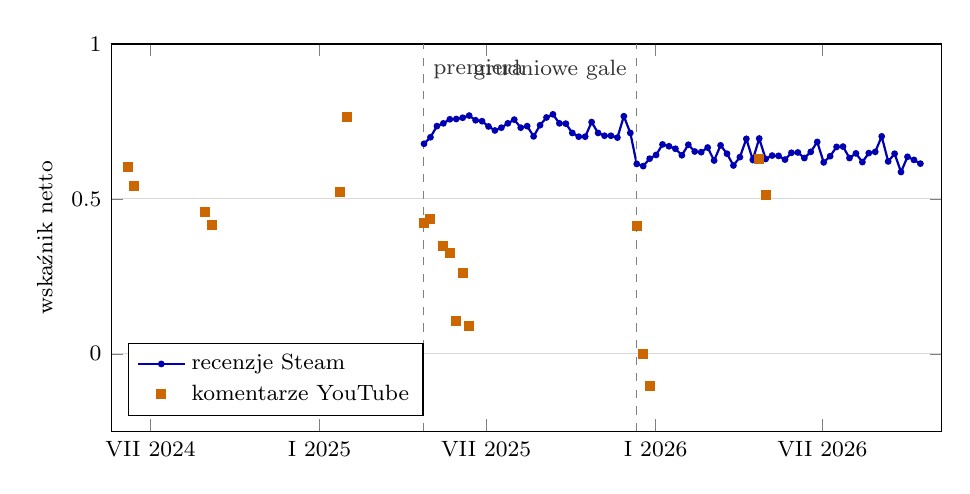
\begin{tikzpicture}
    \begin{axis}[
        font=\footnotesize,
        width=\textwidth, height=6.5cm,
        xmin=2024.38, xmax=2026.85,
        ymin=-0.25, ymax=1.0,
        xtick={2024.4973,2025.0,2025.4959,2026.0,2026.4959},
        xticklabels={VII 2024, I 2025, VII 2025, I 2026, VII 2026},
        ylabel={wskaźnik netto},
        ymajorgrids, grid style={gray!30},
        legend style={at={(0.02,0.04)}, anchor=south west, font=\footnotesize},
        legend cell align=left]
      \addplot[blue!70!black, thick, mark=*, mark size=0.8pt] coordinates {
        (2025.3110,0.678) (2025.3301,0.699) (2025.3493,0.735) (2025.3685,0.744) (2025.3877,0.757) (2025.4068,0.758) (2025.4260,0.762) (2025.4452,0.769) (2025.4644,0.754) (2025.4836,0.751) (2025.5027,0.734) (2025.5219,0.721) (2025.5411,0.730) (2025.5603,0.744) (2025.5795,0.756) (2025.5986,0.730) (2025.6178,0.735) (2025.6370,0.702) (2025.6562,0.738) (2025.6753,0.763) (2025.6945,0.773) (2025.7137,0.744) (2025.7329,0.743) (2025.7521,0.713) (2025.7712,0.701) (2025.7904,0.701) (2025.8096,0.748) (2025.8288,0.713) (2025.8479,0.704) (2025.8671,0.704) (2025.8863,0.698) (2025.9055,0.767) (2025.9247,0.713) (2025.9438,0.613) (2025.9630,0.606) (2025.9822,0.630) (2026.0014,0.642) (2026.0205,0.676) (2026.0397,0.670) (2026.0589,0.662) (2026.0781,0.641) (2026.0973,0.675) (2026.1164,0.653) (2026.1356,0.651) (2026.1548,0.666) (2026.1740,0.624) (2026.1932,0.673) (2026.2123,0.646) (2026.2315,0.608) (2026.2507,0.635) (2026.2699,0.694) (2026.2890,0.626) (2026.3082,0.695) (2026.3274,0.629) (2026.3466,0.640) (2026.3658,0.639) (2026.3849,0.627) (2026.4041,0.649) (2026.4233,0.650) (2026.4425,0.632) (2026.4616,0.652) (2026.4808,0.684) (2026.5000,0.618) (2026.5192,0.638) (2026.5384,0.668) (2026.5575,0.669) (2026.5767,0.632) (2026.5959,0.647) (2026.6151,0.619) (2026.6342,0.648) (2026.6534,0.652) (2026.6726,0.702) (2026.6918,0.621) (2026.7110,0.646) (2026.7301,0.587) (2026.7493,0.636) (2026.7685,0.626) (2026.7877,0.614)};
      \addlegendentry{recenzje Steam}
      \addplot[orange!80!black, only marks, mark=square*, mark size=1.6pt] coordinates {
        (2024.4304,0.602) (2024.4495,0.543) (2024.6599,0.457) (2024.6790,0.417) (2025.0616,0.522) (2025.0808,0.764) (2025.3110,0.421) (2025.3301,0.435) (2025.3685,0.349) (2025.3877,0.326) (2025.4068,0.106) (2025.4260,0.261) (2025.4452,0.091) (2025.9438,0.414) (2025.9630,-0.001) (2025.9822,-0.104) (2026.3082,0.628) (2026.3274,0.514)};
      \addlegendentry{komentarze YouTube}
      \draw[gray, dashed] (axis cs:2025.3096,-0.25) -- (axis cs:2025.3096,1.0);
      \draw[gray, dashed] (axis cs:2025.9425,-0.25) -- (axis cs:2025.9425,1.0);
      \node[anchor=north west, font=\footnotesize, gray!40!black] at (axis cs:2025.3096,0.98) {premiera};
      \node[anchor=north east, font=\footnotesize, gray!40!black] at (axis cs:2025.9425,0.98) {grudniowe gale};
    \end{axis}
  \end{tikzpicture}
  \caption{Tygodniowy wskaźnik wydźwięku netto według źródeł; pokazano tygodnie z co najmniej 20 opiniami}
  \label{fig:weekly-net}
\end{figure}

Wykres pokazuje trzy rzeczy.
Po pierwsze, nastroje na Steam rosły przez pierwsze tygodnie po premierze, od \num{0.68} w tygodniu premiery do \num{0.77} w czerwcu 2025~r., co zgadza się z falą uznania krytyków.
Po drugie, grudzień 2025~r. przyniósł na Steam wyraźny i trwały spadek, z \num{0.71} do \num{0.61}, a wskaźnik do końca okresu nie wrócił do poziomu sprzed gal i w 2026~r. utrzymywał się w przedziale od \num{0.59} do \num{0.70}.
Po trzecie, komentarze YouTube reagują znacznie silniej niż recenzje: w grudniu wskaźnik spadł z \num{0.41} do $-\num{0.10}$.
Na YouTube każde wydarzenie to inny zestaw filmów, więc część tej zmienności wynika z doboru materiału, a nie tylko z nastrojów.

Na wykresie widać też jedną anomalię.
W tygodniu rozpoczynającym się 24 listopada 2025~r. na Steam napisano \num{30653} recenzje, dziesięć razy więcej niż w sąsiednich tygodniach, ze wskaźnikiem netto \num{0.767}.
Ten tydzień nie wiąże się z żadnym z dwunastu wydarzeń w konfiguracji.
\todo{Ustalić przyczynę skoku liczby recenzji w tygodniu od 24.11.2025 (np. promocja w sklepie lub nominacje do nagród) i rozważyć dodanie wydarzenia.}

Efekt poszczególnych wydarzeń względem tła z tego samego źródła przedstawia rysunek~\ref{fig:event-lift}.

\begin{figure}[hbp]
  \centering
  \begin{tikzpicture}
    \begin{axis}[
        font=\footnotesize,
        xbar, bar width=2.4mm,
        width=0.62\textwidth, height=9.5cm,
        y dir=reverse,
        symbolic y coords={reveal,flying,dd,launch,ai,million,critical,tga,iga,anniv},
        ytick={reveal,flying,dd,launch,ai,million,critical,tga,iga,anniv},
        yticklabels={zapowiedź, zwiastun \enquote{Flying Waters}, Xbox Developer Direct, premiera, spór o tekstury AI, milion egzemplarzy, uznanie krytyków, The Game Awards 2025, Indie Game Awards, aktualizacja rocznicowa},
        xmin=-0.65, xmax=0.4,
        xlabel={zmiana wskaźnika netto względem tła},
        xmajorgrids, grid style={gray!30},
        enlarge y limits=0.06,
        legend style={at={(0.02,0.98)}, anchor=north west, font=\footnotesize},
        legend cell align=left]
      \addplot[fill=blue!45, draw=blue!60!black] coordinates {
        (-0.026,launch) (-0.032,ai) (-0.034,million) (0.034,critical) (-0.094,tga) (-0.104,iga) (-0.029,anniv)};
      \addlegendentry{Steam}
      \addplot[fill=orange!60, draw=orange!70!black] coordinates {
        (0.302,reveal) (0.179,flying) (0.307,dd) (0.139,launch) (0.137,million) (-0.044,critical) (0.163,tga) (-0.566,iga) (0.295,anniv)};
      \addlegendentry{YouTube}
      \draw[black] (axis cs:0,reveal) -- (axis cs:0,anniv);
    \end{axis}
  \end{tikzpicture}
  \caption{Efekt wydarzeń: różnica wskaźnika netto w oknie wydarzenia i w tle z tego samego źródła}
  \label{fig:event-lift}
\end{figure}

Na Steam najsilniejszy negatywny efekt miały dwa grudniowe wydarzenia: wokół The Game Awards wskaźnik był o \num{0.094} niższy od tła, a wokół decyzji Indie Game Awards o \num{0.104}.
Jedynym oknem lepszym od tła była fala uznania krytyków, z różnicą \num{0.034}.
Premiera i kilka dni po niej to przede wszystkim lawina opinii, z liczbą recenzji na dzień \num{8.5} raza większą niż w tle, przy niemal niezmienionym wydźwięku.

Na YouTube największy efekt w całym zbiorze ma decyzja Indie Game Awards: wskaźnik netto spadł do $-\num{0.108}$ wobec \num{0.458} w tle, czyli o \num{0.566}.
To jedyne wydarzenie, przy którym komentarze negatywne przeważyły nad pozytywnymi.
Najlepiej przyjęte były zapowiedź gry, pokaz na Xbox Developer Direct i aktualizacja rocznicowa, z efektem około $+\num{0.30}$.
Ciekawy jest przypadek The Game Awards, przy którym źródła rozjechały się w przeciwnych kierunkach: komentarze pod filmami z gali były lepsze od tła YouTube o \num{0.163}, a recenzje Steam z tego okresu gorsze od tła Steam o \num{0.094}.
Jedno z możliwych wyjaśnień jest takie, że komentujący materiały z gali świętowali zwycięstwa, a recenzje z tego samego okresu pisały w dużej części osoby, które sięgnęły po grę pod wpływem nagród i oceniały ją surowiej.
To hipoteza, której nasze dane nie rozstrzygają.

Zestawienie z rekomendacjami autorów z podrozdziału~\ref{sec:eval-weak-labels} wzmacnia te obserwacje dla Steam, bo spadek wokół grudniowych gal widać także w deklaracjach autorów, niezależnych od modelu: udział rekomendacji spadł z \qty{96.2}{\percent} w okresie uznania krytyków do \qty{87.6}{\percent} wokół The Game Awards.

\section{Spełnienie kryteriów akceptacji}
\label{sec:eval-acceptance}

Tabela~\ref{tab:acceptance} zestawia kryteria akceptacji ze specyfikacji wymagań z wynikami opisanymi w tym rozdziale.

\begin{table}[hbp]
  \caption{Kryteria akceptacji i stan ich spełnienia}
  \label{tab:acceptance}
  \centering
  \small
  \begin{tabular}{|p{0.27\textwidth}|p{0.47\textwidth}|p{0.13\textwidth}|}
    \hline
    Kryterium                          & Wynik                                                                                                                & Stan          \\
    \hline
    przebieg od źródła do panelu       & \num{263893} opinii z dwóch źródeł w tabeli zdarzeń, bez błędnych komunikatów, wyniki na panelu; brak formalnego pokazu dla promotora & częściowo \\
    \hline
    test powtarzalności                & identyczny odcisk dla zaślepki; zmiana etykiety dla \qty{0.028}{\percent} opinii przy modelu (próg \qty{0.1}{\percent})   & spełnione     \\
    \hline
    raport jakości modelu              & ocena na części kontrolnej zbioru wzorcowego i na rekomendacjach autorów Steam, porównanie z poprzednimi wersjami       & spełnione     \\
    \hline
    zgodność infrastruktury z kodem    & do potwierdzenia przed złożeniem pracy                                                                                & do sprawdzenia \\
    \hline
  \end{tabular}
\end{table}

\todo[inline]{Uruchomić terraform plan na środowisku dev i wpisać wynik do tabeli; zorganizować pokaz panelu dla promotora.}
Podsumowanie tego, co z tych wyników wynika dla celu pracy, zawiera następny rozdział.

% !TeX root = ../main.tex
\chapter{Podsumowanie}
\label{chap:summary}

% FIRST DRAFT. Future work follows docs/phase-3-plan.md and the open items
% in the phase write-ups.

Zbudowaliśmy system, który pobrał ponad ćwierć miliona opinii o jednej grze z dwóch serwisów, odtworzył je jako strumień w ich rzeczywistej kolejności, sklasyfikował wydźwięk każdej z nich wielojęzycznym modelem i pokazał, jak nastroje zmieniały się wokół dwunastu wydarzeń z życia gry.
Ten rozdział zestawia to, co udało się zrobić, z celem postawionym we wstępie, opisuje ograniczenia, o których czytelnik wyników powinien wiedzieć, i wskazuje, dokąd system warto rozwijać.

\section{Realizacja celów}
\label{sec:summary-goals}

Pierwsze zadanie, pozyskanie opinii z dwóch źródeł z pseudonimizacją autorów, zrealizowaliśmy w zmienionej formie.
Drugim źródłem miał być Reddit, ale po odmowie dostępu zastąpiły go recenzje Steam, które okazały się źródłem lepszym, bo dały rekomendacje autorów jako słabe etykiety.
Zbiór liczy \num{12254} komentarze YouTube z dziewięciu wydarzeń i \num{251639} recenzji Steam, a żaden identyfikator autora nie trafił do zapisu w chmurze.

Drugie i trzecie zadanie, odtwarzanie archiwum w globalnej kolejności chronologicznej i potok przetwarzania strumieniowego, zrealizowaliśmy w całości.
Kolejność sprawdziliśmy bezpośrednio, a powtarzalność odciskiem tabeli, który był identyczny dla dwóch odtworzeń i przetrwał zmianę sposobu uruchamiania.
Pełny zbiór przechodzi przez system w nieco ponad dwie godziny, a jedno odtworzenie to jedno polecenie, po którym system sam sprząta po sobie najdroższe zasoby.

Czwarte zadanie, model z cyklem życia zarządzanym zgodnie z praktykami \ac{mlops}, zrealizowaliśmy, choć droga była dłuższa, niż planowaliśmy.
Angielski DistilBERT okazał się bezużyteczny dla danych wielojęzycznych, więc zastąpiliśmy go modelem XLM-R, dostrojonym w dwóch etapach, w całości na procesorach.
Przebiegi trenowania są zarejestrowane na serwerze MLflow, wersje modeli w rejestrze Agent Platform, a o zastąpieniu wersji decydują spisane przed treningiem warunki.

Piąte zadanie, warstwę raportową i panel, zrealizowaliśmy w postaci widoków Dataform testowanych przy każdym wdrożeniu i raportu Data Studio z trzema stronami.
Szóste, ocenę jakości, powtarzalności, wydajności i kosztów, zrealizowaliśmy w większości: brakuje pomiaru przepustowości z prawdziwym modelem i modelu kosztów dla większych premier.
Siódme, studium przypadku, pokazało, że system wychwytuje zmiany nastrojów, które potwierdzają niezależne od modelu deklaracje autorów recenzji: wzrost w okresie uznania krytyków i spadek wokół grudniowych gal.

Celem, którego nie zrealizowaliśmy, jest klasyfikacja emocji, wymieniona w karcie tematu obok klasyfikacji wydźwięku.
\todo{Uzgodnić z promotorem: albo zmiana celu w MojaPG, albo dodanie klasyfikacji emocji (np. na podstawie GoEmotions) przed złożeniem pracy.}

\section{Ograniczenia rozwiązania}
\label{sec:summary-limitations}

Najważniejsze ograniczenia dotyczą danych.
Zbiór recenzji Steam obejmuje \qty{89.6}{\percent} wszystkich recenzji, a brakujące nie są próbą losową, bo pochodzą z ograniczonych końcówek strumieni angielskich.
Komentarze YouTube pochodzą z ręcznie dobranej listy filmów, więc wynik dla wydarzenia zależy także od tego, które filmy wybraliśmy.
Recenzje Steam zaczynają się w dniu premiery, więc nastroje przed premierą znamy tylko z YouTube.
Wykrywanie języka jest deterministyczne, ale na krótkich tekstach często błędne, więc zestawienia dla rzadkich języków trzeba czytać ostrożnie.

Drugą grupą są ograniczenia oceny modelu, opisane szczegółowo w podrozdziale~\ref{sec:eval-quality-limits}.
Zbiór wzorcowy jest mały, zawiera tylko komentarze YouTube, a jego etykiety zaproponował model językowy i zatwierdził człowiek.
Każdą wersję modelu trenowaliśmy raz.
Model wciąż słabo rozpoznaje negatywne opinie wyrażone pośrednio, ironią albo slangiem, i różnie radzi sobie z różnymi językami.

Trzecią grupą są ograniczenia architektury.
Wydawca odtworzeń, publikując pod jednym kluczem porządkującym, przesyła około 50 komunikatów na sekundę; to celowa cena za globalną kolejność, ale ogranicza tempo każdego odtworzenia.
System analizuje dane historyczne odtwarzane jako strumień, a nie dane napływające na bieżąco.
Raport Data Studio istnieje poza repozytorium, a środowisko produkcyjne nie ma jeszcze ani widoków Dataform, ani raportu.
Konfiguracja wydarzeń i filmów jest częścią obrazów kolektorów, więc nowe studium przypadku wymaga ich przebudowania.

\section{Kierunki dalszych prac}
\label{sec:summary-future}

Najbliższym krokiem jest drugie studium przypadku.
System projektowaliśmy z myślą o nim: przedrostek nazw zasobów pozwala utworzyć drugi komplet zasobów obok pierwszego, numer aplikacji Steam jest parametrem, a schemat danych nie zależy od premiery.
Do zrobienia pozostaje przeniesienie konfiguracji wydarzeń z obrazów do Cloud Storage, decyzja, czy premiery mają mieć osobne zbiory danych, czy wspólny z kolumną identyfikującą premierę, oraz osobny zbiór wzorcowy dla nowego tytułu.
Decyzję o zbiorach trzeba podjąć przed zbieraniem danych, bo później oznacza ona zmianę schematu.
\todo{Na osobnej gałęzi powstaje kolektor serwisu Bluesky dla kolejnego studium przypadku; opisać, jeśli zostanie włączony do systemu przed złożeniem pracy.}

Drugim kierunkiem jest analiza w czasie rzeczywistym.
Wymaga ona przyrostowego pobierania danych według harmonogramu i stale działającego potoku, czyli dokładnie tego, przed czym chronią dziś wszystkie zabezpieczenia kosztowe.
Kolektor Steam jest do tego gotowy, bo krótkie okno czasowe oznacza krótkie przejście od najnowszych recenzji, a YouTube przy pobieraniu co 15 minut zmieści się w dziennym limicie, jeśli nie będzie wyszukiwać nowych filmów.
Najtańszą demonstracją byłoby uruchomienie harmonogramu i potoku na godzinę, na przykład na czas obrony.
Odtwarzanie pozostałoby przy tym na swoim miejscu, bo panel na żywo i powtarzalny wynik pracy dyplomowej to dwa różne wymagania.

Trzecim kierunkiem jest jakość modelu.
Najwięcej dałoby więcej oznaczonych przykładów negatywnych z ukrytą negacją i slangiem, niezależne oznaczenie części zbioru wzorcowego przez dwie osoby i trenowanie z kilkoma ziarnami losowymi.
Z rozszerzeń funkcjonalnych naturalne są klasyfikacja emocji i analiza aspektowa, która powiedziałaby nie tylko, że grudniowe recenzje były gorsze, ale też, co w nich krytykowano.

Na koniec wracamy do przykładu ze wstępu.
Spadek nastrojów w grudniu 2025~r. widać w komentarzach, w recenzjach i w deklaracjach autorów, ale każde z tych źródeł pokazuje go inaczej, a jedno z nich w tygodniu gali pokazuje wręcz poprawę.
Odpowiedź na pytanie, który obraz jest prawdziwy, zależy od tego, czyje nastroje chcemy mierzyć, i być może to jest najważniejsza lekcja z tego projektu: zanim zapytamy, co ludzie myślą o premierze, trzeba ustalić, kogo słuchamy.


% --- Back matter --------------------------------------------------------------
\printbibliography[heading=bibintoc, title={Wykaz literatury}]

% Lists: single line spacing, each one in the table of contents.
\begingroup
\singlespacing
\clearpage\phantomsection
\addcontentsline{toc}{chapter}{\listfigurename}
\listoffigures
\clearpage\phantomsection
\addcontentsline{toc}{chapter}{\listtablename}
\listoftables
\clearpage\phantomsection
\addcontentsline{toc}{chapter}{\lstlistlistingname}
\lstlistoflistings
\endgroup

% Appendices (PG: after the lists).
% !TeX root = ../main.tex
\chapter*{Dodatek A. Zapytania użyte w ewaluacji}
\addcontentsline{toc}{chapter}{Dodatek A. Zapytania użyte w ewaluacji}
\label{chap:appendix-queries}

% FIRST DRAFT. The exact queries run on 2026-11-23 (read-only, reporting
% views only: no author hash, no text).

Zapytania z tego dodatku dają wyniki z podrozdziałów~\ref{sec:eval-weak-labels} i~\ref{sec:eval-case-study}.
Wszystkie czytają wyłącznie widoki zbioru raportowego, które nie zawierają pseudonimu autora ani treści opinii, a wykonaliśmy je 23 listopada 2026~r. na danych z odtworzenia z 18 października 2026~r.
Zapytanie z listingu~\ref{lst:q-weak} daje macierz z tabeli~\ref{tab:weak-confusion}.

\begin{lstlisting}[float=hbp, language=SQL, caption={Etykiety modelu a rekomendacje autorów recenzji Steam}, label={lst:q-weak}]
SELECT voted_up, sentiment_label, COUNT(*) AS n
FROM `pop-vibe-check.co_reporting_dev.v_events`
WHERE source = 'steam'
GROUP BY 1, 2
ORDER BY 1, 2;
\end{lstlisting}

Zapytanie z listingu~\ref{lst:q-weak-events} daje zestawienie z tabeli~\ref{tab:weak-events}; po zamianie kolumny grupującej na \code{language} daje też porównanie dla języków.

\begin{lstlisting}[float=hbp, language=SQL, caption={Udział rekomendacji i wskaźnik netto modelu w oknach wydarzeń}, label={lst:q-weak-events}]
SELECT
  IFNULL(event_tag, 'general') AS event_tag,
  COUNT(*) AS n,
  ROUND(AVG(IF(voted_up, 1, 0)), 3) AS thumbs_up_share,
  ROUND(SAFE_DIVIDE(COUNTIF(sentiment_label = 'pos')
                    - COUNTIF(sentiment_label = 'neg'), COUNT(*)), 3) AS net_model
FROM `pop-vibe-check.co_reporting_dev.v_events`
WHERE source = 'steam'
GROUP BY 1
ORDER BY 1;
\end{lstlisting}

Zapytanie z listingu~\ref{lst:q-weekly} daje dane do rysunku~\ref{fig:weekly-net}, a zapytanie z listingu~\ref{lst:q-lift} dane do rysunku~\ref{fig:event-lift}.

\begin{lstlisting}[float=hbp, language=SQL, caption={Tygodniowy wskaźnik netto według źródeł}, label={lst:q-weekly}]
SELECT source, period, records, ROUND(net_sentiment, 3) AS net
FROM `pop-vibe-check.co_reporting_dev.v_sentiment_by_period`
WHERE grain = 'week' AND records >= 20
ORDER BY source, period;
\end{lstlisting}

\begin{lstlisting}[float=hbp, language=SQL, caption={Efekt wydarzeń względem tła z tego samego źródła}, label={lst:q-lift}]
SELECT event_tag, source, records, days,
       ROUND(net_sentiment, 3) AS net,
       ROUND(baseline_net_sentiment, 3) AS base_net,
       ROUND(net_lift, 3) AS lift,
       ROUND(volume_multiplier, 2) AS vol_mult
FROM `pop-vibe-check.co_reporting_dev.v_event_lift`
ORDER BY source, event_tag;
\end{lstlisting}


\end{document}
